% !TeX spellcheck = en-US
% !TeX encoding = utf8
% !TeX program = pdflatex
% !BIB program = biber
% -*- coding:utf-8 mod:LaTeX -*-


% vv  scroll down to line 200 for content  vv


\let\ifdeutsch\iffalse
\let\ifenglisch\iftrue
% EN: This file is loaded before the \documentclass command in the main document

% EN: The following package allows \\ at the title page
%     For more information see https://github.com/latextemplates/scientific-thesis-cover/issues/4
\RequirePackage{kvoptions-patch}

\ifenglisch
  \PassOptionsToClass{numbers=noenddot}{scrbook}
\else
  %()Aus scrguide.pdf - der Dokumentation von KOMA-Script)
  %Nach DUDEN steht in Gliederungen, in denen ausschließlich arabische Ziffern für die Nummerierung
  %verwendet werden, am Ende der Gliederungsnummern kein abschließender Punkt
  %(siehe [DUD96, R3]). Wird hingegen innerhalb der Gliederung auch mit römischen Zahlen
  %oder Groß- oder Kleinbuchstaben gearbeitet, so steht am Ende aller Gliederungsnummern ein
  %abschließender Punkt (siehe [DUD96, R4])
  \PassOptionsToClass{numbers=autoendperiod}{scrbook}
\fi

% Warns about outdated packages and missing caption declarations
% See https://www.ctan.org/pkg/nag
\RequirePackage[l2tabu, orthodox]{nag}

%DE: Neue deutsche Trennmuster
%    Siehe http://www.ctan.org/pkg/dehyph-exptl und http://projekte.dante.de/Trennmuster/WebHome
%    Nur für pdflatex, nicht für lualatex
\RequirePackage{ifluatex}
\ifluatex
  % do not load anything
\else
  \ifdeutsch
    \RequirePackage[ngerman=ngerman-x-latest]{hyphsubst}
  \fi
\fi

\documentclass[
  % fontsize=11pt is the standard
  a4paper,  % Standard format - only KOMAScript uses paper=a4 - https://tex.stackexchange.com/a/61044/9075
  twoside,  % we are optimizing for both screen and two-side printing. So the page numbers will jump, but the content is configured to stay in the middle (by using the geometry package)
  bibliography=totoc,
  %               idxtotoc,   %Index ins Inhaltsverzeichnis
  %               liststotoc, %List of X ins Inhaltsverzeichnis, mit liststotocnumbered werden die Abbildungsverzeichnisse nummeriert
  headsepline,
  cleardoublepage=empty,
  parskip=half,
  %               draft    % um zu sehen, wo noch nachgebessert werden muss - wichtig, da Bindungskorrektur mit drin
  draft=false
]{scrbook}
% !TeX encoding = utf8
% -*- coding:utf-8 mod:LaTeX -*-

% EN: This file includes basic packages and sets options. The order of package
%     loading is important

% DE: In dieser Datei werden zuerst die benoetigten Pakete eingebunden und
%     danach diverse Optionen gesetzt. Achtung Reihenfolge ist entscheidend!


% EN: Styleguide:
% - English comments are prefixed with "EN", German comments are prefixed with "DE"
% - Prefixed headings define the language for the subsequent paragraphs
% - It is tried to organize packages in blocks. Bocks are separated by two empty lines.

% DE: Styleguide:
%
% Ein sehr kleiner Styleguide. Packages werden in Blöcken organisiert.
% Zwischen zwei Blöcken sind 2 Leerzeilen!


% EN: Enable copy and paste of text from the PDF
%     Only required for pdflatex. It "just works" in the case of lualatex.
%     mmap enables mathematical symbols, but does not work with the newtx font set
%     See: https://tex.stackexchange.com/a/64457/9075
%     Other solutions outlined at http://goemonx.blogspot.de/2012/01/pdflatex-ligaturen-und-copynpaste.html and http://tex.stackexchange.com/questions/4397/make-ligatures-in-linux-libertine-copyable-and-searchable
%     Trouble shooting outlined at https://tex.stackexchange.com/a/100618/9075

\ifluatex
\else
  \usepackage{cmap}
\fi


% EN: File encoding
% DE: Codierung
%     Wir sind im 21 Jahrhundert, utf-8 löst so viele Probleme.
%
% Mit UTF-8 funktionieren folgende Pakete nicht mehr. Bitte beachten!
%   * fancyvrb mit §
%   * easylist -> http://www.ctan.org/tex-archive/macros/latex/contrib/easylist/
\ifluatex
  % EN: See https://tex.stackexchange.com/a/158517/9075
  %     Not required, because of usage of fontspec package
  %\usepackage[utf8]{luainputenc}
\else
  \usepackage[utf8]{inputenc}
\fi


% DE: Parallelbetrieb tex4ht und pdflatex

\makeatletter
\@ifpackageloaded{tex4ht}{
  \def\iftex4ht{\iftrue}
}{
  \def\iftex4ht{\iffalse}
}
\makeatother


% EN: Mathematics
% DE: Mathematik
%
% DE: Viele Mathematik-Sachen. Siehe https://texdoc.net/pkg/amsmath
%
% EN: Options must be passed this way, otherwise it does not work with glossaries
% DE: fleqn (=Gleichungen linksbündig platzieren) funktioniert nicht direkt. Es muss noch ein Patch gemacht werden:
\PassOptionsToPackage{fleqn,leqno}{amsmath}
%
% DE: amsmath Muss nicht mehr geladen werden, da es von newtxmath automatisch geladen wird
% \usepackage{amsmath}


%% EN: Fonts
%% DE: Schriften
%%
%% !!! If you change the font, be sure that words such as "workflow" can
%% !!! still be copied from the PDF. If this is not the case, you have
%% !!! to use glyphtounicode. See comment at cmap package


% EN: Times Roman for all text
\ifluatex
  \RequirePackage{amsmath}
  \RequirePackage{unicode-math}
  \setmainfont{TeX Gyre Termes}
  \setmathfont{texgyretermes-math.otf}
  \setsansfont[Scale=.9]{TeX Gyre Heros}
  \setmonofont[StylisticSet={1,3},Scale=.9]{inconsolata}
\else
  \RequirePackage{newtxtext}
  \RequirePackage{newtxmath}
  % EN: looks good with times, but no equivalent for lualatex found,
  %     therefore replaced with inconsolata
  %\RequirePackage[zerostyle=b,scaled=.9]{newtxtt}
  \RequirePackage[varl,scaled=.9]{inconsolata}

  % DE: Symbole
  % unicode-math scheint für die meisten schon etwas anzubieten
  %
  %\usepackage[geometry]{ifsym} % \BigSquare

  % EN: The euro sign
  % DE: Das Euro Zeichen
  %     Fuer Palatino (mathpazo.sty): richtiges Euro-Zeichen
  %     Alternative: \usepackage{eurosym}
  \newcommand{\EUR}{\ppleuro}
\fi


% DE: Noch mehr Symbole
%\usepackage{stmaryrd} %fuer \ovee, \owedge, \otimes
%\usepackage{marvosym} %fuer \Writinghand %patched to not redefine \Rightarrow
%\usepackage{mathrsfs} %mittels \mathscr{} schoenen geschwungenen Buchstaben erzeugen
%\usepackage{calrsfs} %\mathcal{} ein bisserl dickeren buchstaben erzeugen - sieht net so gut aus.

% EN: Fallback font - if the subsequent font packages do not define a font (e.g., monospaced)
%     This is the modern package for "Computer Modern".
%     In case this gets activated, one has to switch from cmap package to glyphtounicode (in the case of pdflatex)
% DE: Fallback-Schriftart
%\usepackage[%
%    rm={oldstyle=false,proportional=true},%
%    sf={oldstyle=false,proportional=true},%
%    tt={oldstyle=false,proportional=true,variable=true},%
%    qt=false%
%]{cfr-lm}

% EN: Headings are typset in Helvetica (which is similar to Arial)
% DE: Schriftart fuer die Ueberschriften - ueberschreibt lmodern
%\usepackage[scaled=.95]{helvet}

% DE: Für Schreibschrift würde tun, muss aber nicht
%\usepackage{mathrsfs} %  \mathscr{ABC}

% EN: Font for the main text
% DE: Schriftart fuer den Fliesstext - ueberschreibt lmodern
%     Linux Libertine, siehe http://www.linuxlibertine.org/
%     Packageparamter [osf] = Minuskel-Ziffern
%     rm = libertine im Brottext, Linux Biolinum NICHT als serifenlose Schrift, sondern helvet (von oben) beibehalten
%\usepackage[rm]{libertine}

% EN: Alternative Font: Palantino. It is recommeded by Prof. Ludewig for German texts
% DE: Alternative Schriftart: Palantino, Packageparamter [osf] = Minuskel-Ziffern
%     Bitte nur in deutschen Texten
%\usepackage{mathpazo} %ftp://ftp.dante.de/tex-archive/fonts/mathpazo/ - Tipp aus DE-TEX-FAQ 8.2.1

% DE: Schriftart fuer Programmcode - ueberschreibt lmodern
%     Falls auskommentiert, wird die Standardschriftart lmodern genommen
%     Fuer schreibmaschinenartige Schluesselwoerter in den Listings - geht bei alten Installationen nicht, da einige Fontshapes (<>=) fehlen
%\usepackage[scaled=.92]{luximono}
%\usepackage{courier}
% DE: BeraMono als Typewriter-Schrift, Tipp von http://tex.stackexchange.com/a/71346/9075
%\usepackage[scaled=0.83]{beramono}

% EN: backticks (`) are rendered as such in verbatim environments.
%     See following links for details:
%     - https://tex.stackexchange.com/a/341057/9075
%     - https://tex.stackexchange.com/a/47451/9075
%     - https://tex.stackexchange.com/a/166791/9075
\usepackage{upquote}

% EN: For \texttrademark{}
\usepackage{textcomp}

% EN: name-clashes von marvosym und mathabx vermeiden:
\def\delsym#1{%
  %  \expandafter\let\expandafter\origsym\expandafter=\csname#1\endcsname
  %  \expandafter\let\csname orig#1\endcsname=\origsym
  \expandafter\let\csname#1\endcsname=\relax
}

%\usepackage{pifont}
%\usepackage{bbding}
%\delsym{Asterisk}
%\delsym{Sun}\delsym{Mercury}\delsym{Venus}\delsym{Earth}\delsym{Mars}
%\delsym{Jupiter}\delsym{Saturn}\delsym{Uranus}\delsym{Neptune}
%\delsym{Pluto}\delsym{Aries}\delsym{Taurus}\delsym{Gemini}
%\delsym{Rightarrow}
%\usepackage{mathabx} - Ueberschreibt leider zu viel - und die \le-Zeichen usw. sehen nicht gut aus!


% EN: Modern font encoding
%     Has to be loaded AFTER any font packages. See https://tex.stackexchange.com/a/2869/9075.
\ifluatex
\else
  \usepackage[T1]{fontenc}
\fi
%


% EN: Character protrusion and font expansion. See http://www.ctan.org/tex-archive/macros/latex/contrib/microtype/
% DE: Optischer Randausgleich und Grauwertkorrektur

\usepackage[
  babel=true, % EN: Enable language-specific kerning. Take language-settings from the languge of the current document (see Section 6 of microtype.pdf)
  expansion=alltext,
  protrusion=alltext-nott, % EN: Ensure that at listings, there is no change at the margin of the listing
  final % EN: Always enable microtype, even if in draft mode. This helps finding bad boxes quickly.
        %     In the standard configuration, this template is always in the final mode, so this option only makes a difference if "pros" use the draft mode
]{microtype}


% EN: \texttt{test -- test} keeps the "--" as "--" (and does not convert it to an en dash)
\DisableLigatures{encoding = T1, family = tt* }

% DE: fuer microtype
% DE: tracking=true muss als Parameter des microtype-packages mitgegeben werden
% DE: Deaktiviert, da dies bei Algorithmen seltsam aussieht

%\DeclareMicrotypeSet*[tracking]{my}{ font = */*/*/sc/* }%
%\SetTracking{ encoding = *, shape = sc }{ 45 }
% DE: Hier wird festgelegt,
%     dass alle Passagen in Kapitälchen automatisch leicht
%     gesperrt werden.
%     Quelle: http://homepage.ruhr-uni-bochum.de/Georg.Verweyen/pakete.html
%    Deaktiviert, da sonst "BPEL", "BPMN" usw. wirklich komisch aussehen.
%     Macht wohl nur bei geisteswissenschaftlichen Arbeiten Sinn.


% EN: amsmath teaks


% EN: Fixes bugs in AMS math
%     Corrently conflicts with unicode-math
% \usepackage{mathtools}

%\numberwithin{equation}{section}
%\renewcommand{\theequation}{\thesection.\Roman{equation}}

% EN: work-around ams-math problem with align and 9 -> 10. Does not work with glossaries, No visual changes.
%\addtolength\mathindent{1em}


% EN: For theorems, replacement for amsthm
\usepackage[amsmath,hyperref]{ntheorem}
\theorempreskipamount 2ex plus1ex minus0.5ex
\theorempostskipamount 2ex plus1ex minus0.5ex
\theoremstyle{break}
\newtheorem{definition}{Definition}[section]


% CTAN: https://ctan.org/pkg/lccaps
% Doc: http://texdoc.net/pkg/lccaps
%
% Required for DE/EN \initialism
\usepackage{lccaps}


% EN: Defintion of colors. Argument "hyperref" is not used as we do not want to change border colors of links: Links are not colored anymore.
% DE: Farbdefinitionen
\usepackage[dvipsnames]{xcolor}


% EN: Required for custom acronyms/glossaries style.
%     Left aligned Columns in tables with fixed width.
%     See http://tex.stackexchange.com/questions/91566/syntax-similar-to-centering-for-right-and-left
\usepackage{ragged2e}


% DE: Wichtig, ansonsten erscheint "No room for a new \write"
\usepackage{scrwfile}


% EN: Support for language-specific hyphenation
% DE: Neue deutsche Rechtschreibung und Literatur statt "Literature"
%     Die folgende Einstellung ist der Nachfolger von ngerman.sty
\ifdeutsch
  % DE: letzte Sprache ist default, Einbindung von "american" ermöglicht \begin{otherlanguage}{amercian}...\end{otherlanguage} oder \foreignlanguage{american}{Text in American}
  %     Siehe auch http://tex.stackexchange.com/a/50638/9075
  \usepackage[american,main=ngerman]{babel}
  % Ein "abstract" ist eine "Kurzfassung", keine "Zusammenfassung"
  \addto\captionsngerman{%
    \renewcommand\abstractname{Kurzfassung}%
  }
  \ifluatex
    % EN: conditionally disable ligatures. See https://github.com/latextemplates/scientific-thesis-template/issues/54
    %     for a discussion
    \usepackage[ngerman]{selnolig}
  \fi
\else
  % EN: Set English as language and allow to write hyphenated"=words
  %     `american`, `english` and `USenglish` are synonyms for babel package (according to https://tex.stackexchange.com/questions/12775/babel-english-american-usenglish).
  %      "english" has to go last to set it as default language
  \usepackage[ngerman,main=english]{babel}
  % EN: Hint by http://tex.stackexchange.com/a/321066/9075 -> enable "= as dashes
  \addto\extrasenglish{\languageshorthands{ngerman}\useshorthands{"}}
  \ifluatex
    % EN: conditionally disable ligatures. See https://github.com/latextemplates/scientific-thesis-template/issues/54
    %     for a discussion
    \usepackage[english]{selnolig}
  \fi
\fi
%


% EN: For easy quotations: \enquote{text}
%     This package is very smart when nesting is applied, otherwise textcmds (see below) provides a shorter command
%     Note that this package results in a warning when it is loaded before minted (actually fvextra).
% DE: Anführungszeichen
%     Zitate in \enquote{...} setzen, dann werden automatisch die richtigen Anführungszeichen verwendet.
%     Dieses package erzeugt eine Warnung, wenn es vor minted (genauer fvextra) geladen wird.
\usepackage{csquotes}


% EN: For even easier quotations: \qq{text}.
%     Is not smart in the case of nesting, but good enough for the most cases
\usepackage{textcmds}
\ifdeutsch
  % EN: German quotes are different. So do not use the English quotes, but the ones provided by the csquotes package.
  \renewcommand{\qq}[1]{\enquote{#1}}
\fi


% EN: extended enumarations
% DE: erweitertes Enumerate
\usepackage{paralist}


% DE: Gestaltung der Kopf- und Fußteilen

\usepackage[automark]{scrlayer-scrpage}

\automark[section]{chapter}
\setkomafont{pageheadfoot}{\normalfont\sffamily}
\setkomafont{pagenumber}{\normalfont\sffamily}

% DE: funktioniert nicht: Alle Linien sind hier weg
%\setheadsepline[.4pt]{.4pt}


% DE: Intelligentes Leerzeichen um hinter Abkürzungen die richtigen Abstände zu erhalten, auch leere.
%     Siehe commands.tex \gq{}
\usepackage{xspace}
% DE: Macht \xspace und \enquote kompatibel
\makeatletter
\xspaceaddexceptions{\grqq \grq \csq@qclose@i \} }
\makeatother


\newcommand{\eg}{e.\,g.,\ }
\newcommand{\ie}{i.\,e.,\ }


% EN: introduce \powerset - hint by http://matheplanet.com/matheplanet/nuke/html/viewtopic.php?topic=136492&post_id=997377
\DeclareFontFamily{U}{MnSymbolC}{}
\DeclareSymbolFont{MnSyC}{U}{MnSymbolC}{m}{n}
\DeclareFontShape{U}{MnSymbolC}{m}{n}{
  <-6>    MnSymbolC5
  <6-7>   MnSymbolC6
  <7-8>   MnSymbolC7
  <8-9>   MnSymbolC8
  <9-10>  MnSymbolC9
  <10-12> MnSymbolC10
  <12->   MnSymbolC12%
}{}
\DeclareMathSymbol{\powerset}{\mathord}{MnSyC}{180}


% EN: Package for the appendix
% DE: Anhang
\usepackage{appendix}
%[toc,page,title,header]
%


% EN: Graphics
% DE: Grafikeinbindungen
%
% EN: The parameter "pdftex" is not required
\usepackage{graphicx}
\graphicspath{{\getgraphicspath}}
\newcommand{\getgraphicspath}{graphics/}


% EN: Enables inclusion of SVG graphics - 1:1 approach
%    This is NOT the approach of https://ctan.org/pkg/svg-inkscape,
%     which allows text in SVG to be typeset using LaTeX
%     We just include the SVG as is.
\usepackage{epstopdf}
\epstopdfDeclareGraphicsRule{.svg}{pdf}{.pdf}{%
  inkscape -z -D --file=#1 --export-pdf=\OutputFile
}


% EN: Enables inclusion of SVG graphics - text-rendered-with-LaTeX-approach
%     This is the approach of https://ctan.org/pkg/svg-inkscape,
\newcommand{\executeiffilenewer}[3]{%
  \IfFileExists{#2}
  {
    %\message{file #2 exists}
    \ifnum\pdfstrcmp{\pdffilemoddate{#1}}%
      {\pdffilemoddate{#2}}>0%
      {\immediate\write18{#3}}
    \else
      {%\message{file up to date #2}
      }
    \fi%
  }{
    %\message{file #2 doesn't exist}
    %\message{argument: #3}
    %\immediate\write18{echo "test" > xoutput.txt}
    \immediate\write18{#3}
  }
}
\newcommand{\includesvg}[1]{%
  \executeiffilenewer{#1.svg}{#1.pdf}%
  {
    inkscape -z -D --file=\getgraphicspath#1.svg %
    --export-pdf=\getgraphicspath#1.pdf --export-latex}%
  \input{\getgraphicspath#1.pdf_tex}%
}


% EN: Enable typesetting values with SI units.
\ifdeutsch
  \usepackage[mode=text,group-minimum-digits=4]{siunitx}
  \sisetup{locale=DE}
\else
  \usepackage[mode=text,group-minimum-digits=4,group-separator={,}]{siunitx}
  \sisetup{locale=US}
\fi


% EN: Extensions for tables
% DE: Tabellenerweiterungen
\usepackage{array} %increases tex's buffer size and enables ``>'' in tablespecs
\usepackage{longtable}
\usepackage{dcolumn} %Aligning numbers by decimal points in table columns
\ifdeutsch
  \newcolumntype{d}[1]{D{.}{,}{#1}}
\else
  \newcolumntype{d}[1]{D{.}{.}{#1}}
\fi
\setlength{\extrarowheight}{1pt}


% DE: Eine Zelle, die sich über mehrere Zeilen erstreckt.
%     Siehe Beispieltabelle in Kapitel 2
\usepackage{multirow}


% DE: Fuer Tabellen mit Variablen Spaltenbreiten
%\usepackage{tabularx}
%\usepackage{tabulary}


% EN: Links behave as they should. Enables "\url{...}" for URL typesettings.
%     Allow URL breaks also at a hyphen, even though it might be confusing: Is the "-" part of the address or just a hyphen?
%     See https://tex.stackexchange.com/a/3034/9075.
% DE: Links verhalten sich so, wie sie sollen
%     Zeilenumbrüche bei URLs auch bei Bindestrichen erlauben, auch wenn es verwirrend sein könnte: Gehört der Bindestrich zur URL oder ist es ein Trennstrich?
%     Siehe https://tex.stackexchange.com/a/3034/9075.
\usepackage[hyphens]{url}
%
%  EN: When activated, use text font as url font, not the monospaced one.
%      For all options see https://tex.stackexchange.com/a/261435/9075.
% \urlstyle{same}
%
% EN: Hint by http://tex.stackexchange.com/a/10419/9075.
\makeatletter
\g@addto@macro{\UrlBreaks}{\UrlOrds}
\makeatother


% DE: Index über Begriffe, Abkürzungen
%\usepackage{makeidx} makeidx ist out -> http://xindy.sf.net verwenden


% DE: lustiger Hack fuer das Abkuerzungsverzeichnis
%     nach latex durchlauf folgendes ausfuehren
%     makeindex ausarbeitung.nlo -s nomencl.ist -o ausarbeitung.nls
%     danach nochmal latex
%\usepackage{nomencl}
%    \let\abk\nomenclature %Deutsche Ueberschrift setzen
%          \renewcommand{\nomname}{List of Abbreviations}
%        %Punkte zw. Abkuerzung und Erklaerung
%          \setlength{\nomlabelwidth}{.2\hsize}
%          \renewcommand{\nomlabel}[1]{#1 \dotfill}
%        %Zeilenabstaende verkleinern
%          \setlength{\nomitemsep}{-\parsep}
%    \makenomenclature


% EN: Logic for TeX - enables if-then-else in commands
% DE: Logik für TeX
%     FÜr if-then-else @ commands.tex
\usepackage{ifthen}


% EN: Code Listings
% DE: Listings
\usepackage{listings}
\lstset{language=XML,
  showstringspaces=false,
  extendedchars=true,
  basicstyle=\footnotesize\ttfamily,
  commentstyle=\slshape,
  % DE: Original: \rmfamily, damit werden die Strings im Quellcode hervorgehoben. Zusaetzlich evtl.: \scshape oder \rmfamily durch \ttfamily ersetzen. Dann sieht's aus, wie bei fancyvrb
  stringstyle=\ttfamily,
  breaklines=true,
  breakatwhitespace=true,
  % EN: alternative: fixed
  columns=flexible,
  numbers=left,
  numberstyle=\tiny,
  basewidth=.5em,
  xleftmargin=.5cm,
  % aboveskip=0mm, %DE: deaktivieren, falls man lstlistings direkt als floating object benutzt (\begin{lstlisting}[float,...])
  % belowskip=0mm, %DE: deaktivieren, falls man lstlistings direkt als floating object benutzt (\begin{lstlisting}[float,...])
  captionpos=b
}

\ifluatex
\else
  % EN: Enable UTF-8 support - see https://tex.stackexchange.com/q/419327/9075
  \usepackage{listingsutf8}
  \lstset{inputencoding=utf8/latin1}
\fi

\ifdeutsch
  \renewcommand{\lstlistlistingname}{Verzeichnis der Listings}
\fi


% EN: Alternative to listings could be fancyvrb. Can be used together.
% DE: Alternative zu Listings ist fancyvrb. Kann auch beides gleichzeitig benutzt werden.
\usepackage{fancyvrb}
%
% EN: Font size for the normal text
% DE: Groesse fuer den Fliesstext. Falls deaktiviert: \normalsize
%\fvset{fontsize=\small}
%
% DE: Somit kann im Text ganz einfach §verbatim§ text gesetzt werden.
%     Disabled, because UTF-8 does not work any more and lualatex causes issues
%\DefineShortVerb{\§}
%
% EN: Shrink font size of listings
\RecustomVerbatimEnvironment{Verbatim}{Verbatim}{fontsize=\footnotesize}
\RecustomVerbatimCommand{\VerbatimInput}{VerbatimInput}{fontsize=\footnotesize}
%
% EN: Hack for fancyvrb based on http://newsgroups.derkeiler.com/Archive/Comp/comp.text.tex/2008-12/msg00075.html
%     Change of the solution: \Vref somehow collidated with cleveref/varioref as the output of \Vref{} was "Abschnitt 4.3 auf Seite 85"; therefore changed to \myVref -- so completely removed
%     See https://tex.stackexchange.com/q/132420/9075 for more information.
\newcommand{\Vlabel}[1]{\label[line]{#1}\hypertarget{#1}{}}
\newcommand{\lref}[1]{\hyperlink{#1}{\FancyVerbLineautorefname~\ref*{#1}}}


% EN: Tunings of captions for floats, listings, ...
% DE: Bildunterschriften bei floats genauso formatieren wie bei Listings
%     Anpassung wird unten bei den newfloat-Deklarationen vorgenommen
%     https://www.ctan.org/pkg/caption2 is superseeded by this package.
\usepackage{caption}


% EN: Provides rotating figures, where the PDF page is also turned
% DE: Ermoeglicht es, Abbildungen um 90 Grad zu drehen
%     Alternatives Paket: rotating Allerdings wird hier nur das Bild gedreht, während bei lscape auch die PDF-Seite gedreht wird.
%     Das Paket lscape dreht die Seite auch nicht
\usepackage{pdflscape}


% EN: Required for proper environments of fancyvrb and lstlistings
%    There is also the newfloat pacakge (recommended by minted), but we currently have no expericene with that
% DE: Wird für fancyvrb und für lstlistings verwendet
\usepackage{float}
%
% EN: Alternative to float package
%\usepackage{floatrow}
% DE: zustäzlich für den Paramter [H] = Floats WIRKLICH da wo sie deklariert wurden paltzieren - ganz ohne Kompromisse
%     floatrow ist der Nachfolger von float
%     Allerdings macht floatrow in manchen Konstellationen Probleme. Deshalb ist das Paket deaktiviert.
%
% EN: See http://www.tex.ac.uk/cgi-bin/texfaq2html?label=floats
% DE: floats IMMER nach einer Referenzierung platzieren
%\usepackage{flafter}


% EN: Put footnotes below floats
%     Source: https://tex.stackexchange.com/a/32993/9075
\usepackage{stfloats}
\fnbelowfloat


% EN: For nested figures
% DE: Fuer Abbildungen innerhalb von Abbildungen
%     Ersetzt die Pakete subfigure und subfig - siehe https://tex.stackexchange.com/a/13778/9075
\usepackage[hypcap=true]{subcaption}


% EN: Extended support for footnotes
% DE: Fußnoten
%
%\usepackage{dblfnote}  %Zweispaltige Fußnoten
%
% Keine hochgestellten Ziffern in der Fußnote (KOMA-Script-spezifisch):
%\deffootnote[1.5em]{0pt}{1em}{\makebox[1.5em][l]{\bfseries\thefootnotemark}}
%
% Abstand zwischen Fußnoten vergrößern:
%\setlength{\footnotesep}{.85\baselineskip}
%
% EN: Following command disables the separting line of the footnote
% DE: Folgendes Kommando deaktiviert die Trennlinie zur Fußnote
%\renewcommand{\footnoterule}{}
%
\addtolength{\skip\footins}{\baselineskip} % Abstand Text <-> Fußnote
%
% Fußnoten immer ganz unten auf einer \raggedbottom-Seite
% fnpos kommt aus dem yafoot package
\usepackage{fnpos}
\makeFNbelow
\makeFNbottom


% EN: Variable page heights
% DE: Variable Seitenhöhen zulassen
\raggedbottom


% DE: Falls die Seitenzahl bei einer Referenz auf eine Abbildung nur dann angegeben werden soll,
%     falls sich die Abbildung nicht auf der selben Seite befindet...
\iftex4ht
  %tex4ht does not work well with vref, therefore we emulate vref behavior
  \newcommand{\vref}[1]{\ref{#1}}
\else
  \ifdeutsch
    \usepackage[ngerman]{varioref}
  \else
    \usepackage{varioref}
  \fi
\fi


% EN: More beautiful tables if one uses \toprule, \midrule, \bottomrule
% DE: Noch schoenere Tabellen als mit booktabs mit http://www.zvisionwelt.de/downloads.html
\usepackage{booktabs}
%
%\usepackage[section]{placeins}


% EN: Graphs and Automata
%
% TODO: Since version 3.0 (2013-10-01), it supports pdflatex via the auto-pst-pdf package
%       Requires -shell-escape
%\usepackage{gastex}


%\usepackage{multicol}

% DE: kollidiert mit diplomarbeit.sty
%\usepackage{setspace}


% DE: biblatex statt bibtex
\usepackage[
  backend       = biber, %biber does not work with 64x versions alternative: bibtex8
  %minalphanames only works with biber backend
  sortcites     = true,
  bibstyle      = alphabetic,
  citestyle     = alphabetic,
  giveninits    = true,
  useprefix     = false, %"von, van, etc." will be printed, too. See below.
  minnames      = 1,
  minalphanames = 3,
  maxalphanames = 4,
  maxbibnames   = 99,
  maxcitenames  = 2,
  natbib        = true,
  eprint        = true,
  url           = true,
  doi           = true,
  isbn          = true,
  backref       = true]{biblatex}

% enable more breaks at URLs. See https://tex.stackexchange.com/a/134281.
\setcounter{biburllcpenalty}{7000}
\setcounter{biburlucpenalty}{8000}

\bibliography{bibliography}
%\addbibresource[datatype=bibtex]{bibliography.bib}

%Do not put "vd" in the label, but put it at "\citeauthor"
%Source: http://tex.stackexchange.com/a/30277/9075
\makeatletter
\AtBeginDocument{\toggletrue{blx@useprefix}}
\AtBeginBibliography{\togglefalse{blx@useprefix}}
\makeatother

%Thin spaces between initials
%http://tex.stackexchange.com/a/11083/9075
\renewrobustcmd*{\bibinitdelim}{\,}

%Keep first and last name together in the bibliography
%http://tex.stackexchange.com/a/196192/9075
\renewcommand*\bibnamedelimc{\addnbspace}
\renewcommand*\bibnamedelimd{\addnbspace}

%Replace last "and" by comma in bibliography
%See http://tex.stackexchange.com/a/41532/9075
\AtBeginBibliography{%
  \renewcommand*{\finalnamedelim}{\addcomma\space}%
}

\DefineBibliographyStrings{ngerman}{
  backrefpage  = {zitiert auf S\adddot},
  backrefpages = {zitiert auf S\adddot},
  andothers    = {et\ \addabbrvspace al\adddot},
  %Tipp von http://www.mrunix.de/forums/showthread.php?64665-biblatex-Kann-%DCberschrift-vom-Inhaltsverzeichnis-nicht-%E4ndern&p=293656&viewfull=1#post293656
  bibliography = {Literaturverzeichnis}
}

% EN: enable hyperlinked author names when using \citeauthor
%     source: http://tex.stackexchange.com/a/75916/9075
\DeclareCiteCommand{\citeauthor}
{\boolfalse{citetracker}%
  \boolfalse{pagetracker}%
  \usebibmacro{prenote}}
{\ifciteindex
  {\indexnames{labelname}}
  {}%
  \printtext[bibhyperref]{\printnames{labelname}}}
{\multicitedelim}
{\usebibmacro{postnote}}

% EN: natbib compatibility
%\newcommand{\citep}[1]{\cite{#1}}
%\newcommand{\citet}[1]{\citeauthor{#1} \cite{#1}}
% EN: Beginning of sentence - analogous to cleveref - important for names such as "zur Muehlen"
%\newcommand{\Citep}[1]{\cite{#1}}
%\newcommand{\Citet}[1]{\Citeauthor{#1} \cite{#1}}

% DE: Blindtext. Paket "blindtext" ist fortgeschritterner als "lipsum" und kann auch Mathematik im Text (http://texblog.org/2011/02/26/generating-dummy-textblindtext-with-latex-for-testing/)
%     kantlipsum (https://www.ctan.org/tex-archive/macros/latex/contrib/kantlipsum) ist auch ganz nett, aber eben auch keine Mathematik
%     Wird verwendet, um etwas Text zu erzeugen, um eine volle Seite wegen Layout zu sehen.
\usepackage[math]{blindtext}


% EN: Make LaTeX logos available by commands. E.g., \lualatex
%     Disabled, because currently causes \not= already defined
%\usepackage{dtk-logos}

% quick replacement:
\newcommand{\LuaLaTeX}{Lua\LaTeX\xspace}
\newcommand{\lualatex}{\LuaLaTeX}

% DE: Neue Pakete bitte VOR hyperref einbinden. Insbesondere bei Verwendung des
%     Pakets "index" wichtig, da sonst die Referenzierung nicht funktioniert.
%     Für die Indizierung selbst ist unter http://xindy.sourceforge.net
%     ein gutes Tool zu erhalten.
%     Hier also neue packages einbinden.
% EN: Add new packages at this place.


% EN: Provides hyperlinks
%     Option "unicode" fixes umlauts in the PDF bookmarks - see https://tex.stackexchange.com/a/338770/9075
%
% DE: Erlaubt Hyperlinks im Dokument.
%     Alle Optionen nach \hypersetup verschoben, sonst crash
%     Siehe auch: "Praktisches LaTeX" - www.itp.uni-hannover.de/~kreutzm
\usepackage[unicode]{hyperref}


% EN: Define colors
% DE: Da es mit KOMA 3 und xcolor zu Problemen mit den global Options kommt MÜSSEN die Optionen so gesetzt werden.
%     Eigene Farbdefinitionen ohne die Namen des xcolor packages
\definecolor{darkblue}{rgb}{0,0,.5}
\definecolor{black}{rgb}{0,0,0}


% EN: Define color of links and more
\hypersetup{
  % have both title and number hyperlinking to content
  linktoc=all,
  bookmarksnumbered=true,
  bookmarksopen=true,
  bookmarksopenlevel=1,
  breaklinks=true,
  colorlinks=true,
  pdfstartview=Fit,
  pdfpagelayout=SinglePage, % DE: Alterntaive: TwoPageRight -- zweiseitige Darstellung: ungerade Seiten rechts im PDF-Viewer - siehe auch http://tex.stackexchange.com/a/21109/9075
  %pdfencoding=utf8, % EN: This is probably the same as passing the option "unicode" at \usepackage{hyperref}
  filecolor=darkblue,
  urlcolor=darkblue,
  linkcolor=black,
  citecolor=black
}


% EN: Abbreviations - has to be loaded after hyperref
% DE: Abkürzungsverzeichnis - muss nach hyperref geladen werden
%
% DE: siehe http://www.dickimaw-books.com/cgi-bin/faq.cgi?action=view&categorylabel=glossaries#glsnewwriteexceeded
\usepackage[acronym,indexonlyfirst,nomain]{glossaries}
\ifdeutsch
  \addto\captionsngerman % DE: siehe https://tex.stackexchange.com/a/154566
  {%
    \renewcommand*{\acronymname}{Abkürzungsverzeichnis}
  }
\else
  \renewcommand*{\acronymname}{List of Abbreviations}
\fi
\renewcommand*{\glsgroupskip}{}
%
% EN: Removed Glossarie as a table as a quick fix to get the template working again
%     See http://tex.stackexchange.com/questions/145579/how-to-print-acronyms-of-glossaries-into-a-table
%
\makenoidxglossaries


% EN: Extensions for references inside the document (\cref{fig:sample}, ...)
% DE: cleveref für cref statt autoref, da cleveref auch bei Definitionen funktioniert
\usepackage[capitalise,nameinlink,noabbrev]{cleveref}
\ifdeutsch
  \crefname{table}{Tabelle}{Tabellen}
  \Crefname{table}{Tabelle}{Tabellen}
  \crefname{figure}{\figurename}{\figurename}
  \Crefname{figure}{Abbildung}{Abbildungen}
  \crefname{equation}{Gleichung}{Gleichungen}
  \Crefname{equation}{Gleichung}{Gleichungen}
  \crefname{theorem}{Theorem}{Theoreme}
  \Crefname{theorem}{Theorem}{Theoreme}
  \crefname{listing}{\lstlistingname}{\lstlistingname}
  \Crefname{listing}{Listing}{Listings}
  \crefname{section}{Abschnitt}{Abschnitte}
  \Crefname{section}{Abschnitt}{Abschnitte}
  \crefname{paragraph}{Abschnitt}{Abschnitte}
  \Crefname{paragraph}{Abschnitt}{Abschnitte}
  \crefname{subparagraph}{Abschnitt}{Abschnitte}
  \Crefname{subparagraph}{Abschnitt}{Abschnitte}
\else
  \crefname{listing}{\lstlistingname}{\lstlistingname}
  \Crefname{listing}{Listing}{Listings}
\fi


% DE: Zur Darstellung von Algorithmen
%     Algorithm muss nach hyperref geladen werden
\usepackage[chapter]{algorithm}
\usepackage[]{algpseudocode}


% DE: Links auf Gleitumgebungen springen nicht zur Beschriftung,
%     Doc: http://mirror.ctan.org/tex-archive/macros/latex/contrib/oberdiek/hypcap.pdf
%     sondern zum Anfang der Gleitumgebung
\usepackage[all]{hypcap}


% DE: Deckblattstyle
%
\ifdeutsch
  \PassOptionsToPackage{language=german}{scientific-thesis-cover}
\else
  \PassOptionsToPackage{language=english}{scientific-thesis-cover}
\fi


% EN: Bugfixes packages
%\usepackage{fixltx2e} %Fuer neueste LaTeX-Installationen nicht mehr benoetigt - bereinigte einige Ungereimtheiten, die auf Grund von Rueckwaertskompatibilitaet beibahlten wurden.
%\usepackage{mparhack} %Fixt die Position von marginpars (die in DAs selten bis gar nicht gebraucht werden}
%\usepackage{ellipsis} %Fixt die Abstaende vor \ldots. Wird wohl auch nicht benoetigt.


% EN: Settings for captions of floats
% DE: Formatierung der Beschriftungen
%
\captionsetup{
  format=hang,
  labelfont=bf,
  justification=justified,
  %single line captions should be centered, multiline captions justified
  singlelinecheck=true
}


% EN: New float environments for listings and algorithms
%
% \floatstyle{ruled} % TODO: enabled or disabled causes no change - listings and algorithms are always ruled
%
\newfloat{Listing}{tbp}{code}[chapter]
\crefname{Listing}{Listing}{Listings}

\newfloat{Algorithmus}{tbp}{alg}[chapter]
\ifdeutsch
  \crefname{Algorithmus}{Algorithmus}{Algorithmus}
\else
  \crefname{Algorithmus}{Algorithm}{Algorithms}
  \floatname{Algorithmus}{Algorithm}
\fi



% EN: Various chapter styles
% DE: unterschiedliche Chapter-Styles
%     u.a. Paket fncychap

% Andere Kapitelueberschriften
% falls einem der Standard von KOMA nicht gefaellt...
% Falls man zurück zu KOMA moechte, dann muss jede der vier folgenden Moeglichkeiten deaktiviert sein.

%\usepackage[Sonny]{fncychap}

%\usepackage[Bjarne]{fncychap}

%\usepackage[Lenny]{fncychap}

%DE: Zur Aktivierung eines der folgenden Möglichkeiten ein Paar von "\iffalse" und "\fi" auskommentieren

\iffalse
  \usepackage[Bjarne]{fncychap}
  \ChNameVar{\Large\sf} \ChNumVar{\Huge} \ChTitleVar{\Large\sf}
  \ChRuleWidth{0.5pt} \ChNameUpperCase
\fi

\iffalse
  \usepackage[Rejne]{fncychap}
  \ChNameVar{\centering\Huge\rm\bfseries}
  \ChNumVar{\Huge}
  \ChTitleVar{\centering\Huge\rm}
  \ChNameUpperCase
  \ChTitleUpperCase
  \ChRuleWidth{1pt}
\fi

\iffalse
  \usepackage{fncychap}
  \ChNameUpperCase
  \ChTitleUpperCase
  \ChNameVar{\raggedright\normalsize} %\rm
  \ChNumVar{\bfseries\Large}
  \ChTitleVar{\raggedright\Huge}
  \ChRuleWidth{1pt}
\fi

\iffalse
  \usepackage[Bjornstrup]{fncychap}
  \ChNumVar{\fontsize{76}{80}\selectfont\sffamily\bfseries}
  \ChTitleVar{\raggedright\Large\sffamily\bfseries}
\fi

% EN: Complete different chapter style - self made

% Innen drin kann man dann noch zwischen
%   * serifenloser Schriftart (eingestellt)
%   * serifenhafter Schriftart (wenn kein zusaetzliches Kommando aktiviert ist) und
%   * Kapitälchen wählen
\iffalse
  \makeatletter
  %\def\thickhrulefill{\leavevmode \leaders \hrule height 1ex \hfill \kern \z@}

  %Fuer Kapitel mit Kapitelnummer
  \def\@makechapterhead#1{%
    \vspace*{10\p@}%
    {\parindent \z@ \raggedright \reset@font
      %Default-Schrift: Serifenhaft (gut fuer englische Dokumente)
      %A) Fuer serifenlose Schrift:
      \fontfamily{phv}\selectfont
      %B) Fuer Kapitaelchen:
      %\fontseries{m}\fontshape{sc}\selectfont
      %C) Fuer ganz "normale" Schrift:
      %\normalfont
      %
      \Large \@chapapp{} \thechapter
      \par\nobreak\vspace*{10\p@}%
      \interlinepenalty\@M
      {\Huge\bfseries\baselineskip3ex
        %Fuer Kapitaelchen folgende Zeile aktivieren:
        %\fontseries{m}\fontshape{sc}\selectfont
        #1\par\nobreak}
      \vspace*{10\p@}%
      \makebox[\textwidth]{\hrulefill}%    \hrulefill alone does not work
      \par\nobreak
      \vskip 40\p@
    }}

  %Fuer Kapitel ohne Kapitelnummer (z.B. Inhaltsverzeichnis)
  \def\@makeschapterhead#1{%
    \vspace*{10\p@}%
    {\parindent \z@ \raggedright \reset@font
      \normalfont \vphantom{\@chapapp{} \thechapter}
      \par\nobreak\vspace*{10\p@}%
      \interlinepenalty\@M
      {\Huge \bfseries %
        %Default-Schrift: Serifenhaft (gut fuer englische Dokumente)
        %A) Fuer serifenlose Schrift folgende Zeile aktivieren:
        \fontfamily{phv}\selectfont
        %B) Fuer Kapitaelchen folgende Zeile aktivieren:
        %\fontseries{m}\fontshape{sc}\selectfont
        #1\par\nobreak}
      \vspace*{10\p@}%
      \makebox[\textwidth]{\hrulefill}%    \hrulefill does not work
      \par\nobreak
      \vskip 40\p@
    }}
  %
  \makeatother
\fi


% DE: Minitoc-Einstellungen
%\dominitoc
%\renewcommand{\mtctitle}{Inhaltsverzeichnis dieses Kapitels}


% EN: Nicer paragraph line placement:
%     - Disable single lines at the start of a paragraph (Schusterjungen)
%     - Disable single lines at the end of a paragraph (Hurenkinder)
%     Normally, this is clubpenalty and widowpenalty, but using a package, it feels more non-hacky
\usepackage[all,defaultlines=3]{nowidow}
%
\displaywidowpenalty = 10000


% EN: Try to get rid of "overfull hbox" things and let text flow batter
%     See also
%       - http://groups.google.de/group/de.comp.text.tex/browse_thread/thread/f97da71d90442816/f5da290593fd647e?lnk=st&q=tolerance+emergencystretch&rnum=5&hl=de#f5da290593fd647e
%       - http://www.tex.ac.uk/cgi-bin/texfaq2html?label=overfull
\tolerance=2000
%
% EN: This could be increased to 20pt
\setlength{\emergencystretch}{3pt}
%
% EN: Suppress hbox warnings if less than 1pt
\setlength{\hfuzz}{1pt}


% EN: Fix names for algorithms in German
% DE: fuer algorithm.sty: - falls Deutsch und nicht Englisch.
\ifdeutsch
  \floatname{algorithm}{Algorithmus}
  \renewcommand{\listalgorithmname}{Verzeichnis der Algorithmen}
\fi




% Float-placements - http://dcwww.camd.dtu.dk/~schiotz/comp/LatexTips/LatexTips.html#figplacement
% and http://people.cs.uu.nl/piet/floats/node1.html
\renewcommand{\topfraction}{0.85}
\renewcommand{\bottomfraction}{0.95}
\renewcommand{\textfraction}{0.1}
\renewcommand{\floatpagefraction}{0.75}
%\setcounter{totalnumber}{5}

% EN: ensure that floats covering a whole page are placed at the top of the page
%    see http://tex.stackexchange.com/a/28565/9075
\makeatletter
\setlength{\@fptop}{0pt}
\setlength{\@fpbot}{0pt plus 1fil}
\makeatother



% DE: Bei Gleichungen nur dann die Nummer zeigen, wenn die Gleichung auch referenziert wird
%     Funktioniert mit MiKTeX Stand 2012-01-13 nicht. Deshalb ist dieser Schalter deaktiviert.
%
%\mathtoolsset{showonlyrefs}


% EN: Margins
% DE: Ränder
%     Viele Moeglichkeiten, die Raender im Dokument einzustellen.
%
%     Satzspiegel neu berechnen. Dokumentation dazu ist in "scrguide.pdf" von KOMA-Skript zu finden
%     Optionen werden bei \documentclass[] in ausarbeitung.tex mitgegeben.
% \typearea[current]{current} %neu berechnen, da neue Schrift eingebunden

%\usepackage{a4}
%\usepackage{a4wide}
%\areaset{170mm}{277mm} %a4:29,7hochx21mbreit

%Wer die Masse direkt eingeben moechte:
%Bei diesem Beispiel wird die Regel nicht beachtet, dass der innere Rand halb so gross wie der aussere Rand und der obere Rand halb so gross wie der untere Rand sein sollte
%\usepackage[inner=2.5cm, outer=2.5cm, includefoot, top=3cm, bottom=1.5cm]{geometry}

% EN: Package geometry to enlarge on page
%
%     Normally, geometry should not be used as the typearea package calculates the margins perfectly for printing
%     However, we want better screen-readable documents where the content does not "jump"
%     Thus, we fix the margins left and right to the same value
%
%     Source: http://www.howtotex.com/tips-tricks/change-margins-of-a-single-page/
%
\usepackage[
  left=3cm,right=3cm,top=2.5cm,bottom=2.5cm,
  headsep=18pt,
  footskip=30pt,
  includehead,
  includefoot
]{geometry}


% EN: Provides todo notes
% DE: schoene TODOs
\ifdeutsch
  \usepackage[colorinlistoftodos,ngerman]{todonotes}
\else
  \usepackage[colorinlistoftodos]{todonotes}
\fi
\setlength{\marginparwidth}{2,5cm}

\let\xtodo\todo
\renewcommand{\todo}[1]{\xtodo[inline,color=black!5]{#1}}
\newcommand{\utodo}[1]{\xtodo[inline,color=green!5]{#1}}
\newcommand{\itodo}[1]{\xtodo[inline]{#1}}


% EN: Enable footnotes in tables.
%     This package superseeds the 1997 package "footnote"
\usepackage{footnotehyper}
% TODO: The footnotehyper author recommends to enclose the respective area with \begin{savenotes} ... \end{savenotes}
\makesavenoteenv{tabular}
\makesavenoteenv{table}
% Reuse of footnotes, see http://tex.stackexchange.com/questions/10102/multiple-references-to-the-same-footnote-with-hyperref-support-is-there-a-bett
\crefformat{footnote}{#2\footnotemark[#1]#3}


% EN: pgfplots (optional if the ppackage is installed)
%     PGFPlots draws high-qual­ity func­tion plots in nor­mal or log­a­rith­mic scal­ing
\IfFileExists{pgfplots.sty}{
  \usepackage{pgfplots}
  % EN: highest version supported by overleaf as of 2018-03-16
  \pgfplotsset{compat=1.14}
}{}


% EN: pgfplotstable (optional if the ppackage is installed)
%     PGFPlots generates tables from csv files
\IfFileExists{pgfplotstable.sty}{
  \usepackage{pgfplotstable}
}{}


% EN: Package for creating graphics programmatically
\usepackage{tikz}


% EN: Package for creating uml diagramms
\usepackage{tikz-uml}


% EN: Forest: apgf/TikZ-based package for drawing linguistic trees - https://ctan.org/pkg/forest
\usepackage{forest}


% EN: Enable PlantUML listings in the environment "plantuml"
\IfFileExists{plantuml.sty}{
  \usepackage[output=latex]{plantuml}
}{}


% EN: Layout: bottoms of pages not aligned to each other
% DE: Der untere Rand darf "flattern"
\raggedbottom


% DE: Wie tief wird das Inhaltsverzeichnis aufgeschlüsselt
% 0 --\chapter
% 1 --\section % fuer kuerzeres Inhaltsverzeichnis verwenden - oder minitoc benutzen
% 2 --\subsection
% 3 --\subsubsection
% 4 --\paragraph
\setcounter{tocdepth}{1}


% EN: Fixes wrong spacing in the TOC.
%     Source: https://tex.stackexchange.com/a/33842/9075 -> comment by esdd
\RedeclareSectionCommand[tocnumwidth=2.8em]{section}


% DE: Angaben in die PDF-Infos uebernehmen
\makeatletter
\hypersetup{
  pdftitle={}, %Titel der Arbeit
  pdfauthor={}, %Author
  pdfkeywords={}, % CR-Klassifikation und ggf. weitere Stichworte
  pdfsubject={}
}
\makeatother


% EN: Higher compression of the output PDF
\pdfcompresslevel=9


% EN: Required for recent version of komascript, as some packges are not that compatible with KOMAScript as they should be
%     Has to be loaded at the *very* end, so we use "\AtEndPreamble" by etoolsbox
\usepackage{etoolbox}
\AtEndPreamble{\usepackage{scrhack}}


% EN: Provide tables over multiple pages
\usepackage{longtable}


% EN: Show LaTeX commands and their results in the document
%     Enables the command \PrintDemo
% See https://github.com/latextemplates/scientific-thesis-template/issues/82 for further discussion
\usepackage{latexdemo}


% DE: Fuer deutsche Texte: Weniger Silbentrennung, mehr Abstand zwischen den Woertern
\ifdeutsch
  \setlength{\emergencystretch}{3em} % Silbentrennung reduzieren durch mehr frei Raum zwischen den Worten
\fi



\usepackage[
  title={GETACAR: A Privacy-Preserving Platform for Ride-Pooling},
  author={Hans Hüppelshäuser},
  type=master,
  institute=iaas, % or other institute names - or just a plain string using {Demo\\Demo...}
  course={M.Sc. Wirtschaftsinformatik},
  examiner={Prof.\ Dr.\ Marco Aiello},
  supervisor={Robin Pesl, \ M.Sc.},
  startdate={March 27, 2023},
  enddate={Septeber 27, 2023}
]{scientific-thesis-cover}

% Hier stehen alle Abkürzungen
\newacronym{pow}{PoW}{Proof of Work}
\newacronym{pos}{PoS}{Proof of Stake}
\newacronym{dpos}{DPoS}{Delegated Proof of Stake}
\newacronym{sumo}{SUMO}{Simulation of Urban MObility}
\newacronym{dapp}{DApp}{Decentralised Applications}
\newacronym{ipfs}{IPFS}{Interplanetary File System}
\newacronym{rsus}{RSUs}{Road Side Units}
\newacronym{osi}{OSI}{Open Source Initiative}


\makeindex

\begin{document}

%tex4ht-Konvertierung verschönern
\iftex4ht
  % tell tex4ht to create picures also for formulas starting with '$'
  % WARNING: a tex4ht run now takes forever!
  \Configure{$}{\PicMath}{\EndPicMath}{}
  %$ % <- syntax highlighting fix for emacs
  \Css{body {text-align:justify;}}

  %conversion of .pdf to .png
  \Configure{graphics*}
  {pdf}
  {\Needs{"convert \csname Gin@base\endcsname.pdf
      \csname Gin@base\endcsname.png"}%
    \Picture[pict]{\csname Gin@base\endcsname.png}%
  }
\fi

%\VerbatimFootnotes %verbatim text in Fußnoten erlauben. Geht normalerweise nicht.

% DE: wird fuer Tabellen benötigt (z.B. >{centering\RBS}p{2.5cm} erzeugt einen zentrierten 2,5cm breiten Absatz in einer Tabelle
\newcommand{\RBS}{\let\\=\tabularnewline}

% EN: To avoid issues with Springer's \mathplus
%     See also http://tex.stackexchange.com/q/212644/9075
\providecommand\mathplus{+}

% DE: typoraphisch richtige Abkürzungen
\newcommand{\zB}{z.\,B.\xspace}
\newcommand{\bzw}{bzw.\xspace}
\newcommand{\usw}{usw.\xspace}
\renewcommand{\dh}{d.\,h.\xspace}

% EN: from hmks makros.tex - \indexify
\newcommand{\toindex}[1]{\index{#1}#1}

% DE: Tipp aus "The Comprehensive LaTeX Symbol List"
\newcommand{\dotcup}{\ensuremath{\,\mathaccent\cdot\cup\,}}

% DE: Anstatt $|x|$ $\abs{x}$ verwenden.
%     Die Betragsstriche skalieren automatisch, falls "x" etwas größer sein sollte...
\newcommand{\abs}[1]{\left\lvert#1\right\rvert}

% DE: für Zitate
\newcommand{\citeS}[2]{\cite[S.~#1]{#2}}
\newcommand{\citeSf}[2]{\cite[S.~#1\,f.]{#2}}
\newcommand{\citeSff}[2]{\cite[S.~#1\,ff.]{#2}}
\newcommand{\vgl}{vgl.\ }
\newcommand{\Vgl}{Vgl.\ }

% EN: For the algorithmic package
\newcommand{\commentchar}{\ensuremath{/\mkern-4mu/}}
\algrenewcommand{\algorithmiccomment}[1]{\hfill $\commentchar$ #1}

% DE: Seitengrößen - Gegen Schusterjungen und Hurenkinder...
\newcommand{\largepage}{\enlargethispage{\baselineskip}}
\newcommand{\shortpage}{\enlargethispage{-\baselineskip}}

\newcommand{\initialism}[1]{%
  \ifdeutsch%
    \textsc{#1}\xspace%
  \else%
    \textlcc{#1}\xspace%
  \fi%
}
\newcommand{\OMG}{\initialism{OMG}}
\newcommand{\BPEL}{\initialism{BPEL}}
\newcommand{\BPMN}{\initialism{BPMN}}
\newcommand{\UML}{\initialism{UML}}

\pagenumbering{arabic}
\Titelblatt

%Eigener Seitenstil fuer die Kurzfassung und das Inhaltsverzeichnis
\deftriplepagestyle{preamble}{}{}{}{}{}{\pagemark}
%Doku zu deftriplepagestyle: scrguide.pdf
\pagestyle{preamble}
\renewcommand*{\chapterpagestyle}{preamble}



%Kurzfassung / abstract
%auch im Stil vom Inhaltsverzeichnis

  \section*{Abstract}
The widespread adoption of autonomous vehicles is expected to lead to an overall increase in traffic. Ride-pooling can counter this downside of an otherwise promising technology, but the majority of current ride-pooling platforms utilise centralised designs that allow companies to collect vast amounts of user data. To solve this problem, we propose the decentralised ride-pooling platform GETACAR that focuses on privacy-preservation. GETACAR utilises blockchain technology to allow for the transparent and immutable tracking of ride processes without exposing personal information to other participants or the platform itself. To realise the platform, we develop its design, define its interactions and create a prototypical implementation. GETACAR is comprised of several components, including a customer and ride provider frontend allowing humans and autonomous vehicles to interact with GETACAR. We introduce an off-chain matching service to find the best possible match between customers and ride providers via a Vickrey auction.  GETACAR also connects with crypto exchanges that allow the platform to use cryptocurrencies for internal transactions while users can still handle payments via fiat currencies.
An authentication service verifies all parties wishing to participate on the platform, ensuring accountability and impeding the use of multiple identities.  To ensure safety across the platforms, a robust rating system is in place that allows all parties to rate each other. In addition, a number of privacy mechanisms are in place to minimise the exposure of personal information, including location cloaking, pseudonyms, and frequently changing wallets. A prototype validates the GETACAR platform design by showcasing the platform's key features, including a fully realised user frontend, the matching service, and smart contracts running on the Ethereum blockchain. All these components are connected and working together, allowing for a customer to request a ride with multiple ride providers bidding on the ride. The implemented matching service determines the winner, and smart contracts manage the overall ride, including the rating process. Both the design of the platform and the prototype showcase the potential of blockchain technology to create next-generation ride-pooling platforms that ensure transparency while preserving privacy.

\cleardoublepage

  \section*{Kurzfassung}
Es ist zu erwarten, dass die Verbreitung autonomer Fahrzeuge zu einem allgemeinen Anstieg des Verkehrsaufkommens führen wird. Ride-Pooling kann diesem Nachteil einer ansonsten vielversprechenden Technologie entgegenwirken, aber aktuelle Ride-Pooling-Plattformen nutzen zentralisierte Designs, die es Unternehmen ermöglichen, große Mengen an Benutzerdaten zu sammeln. Um dieses Problem zu lösen, setzt die dezentrale Ride-Pooling-Plattform GETACAR auf den Schutz der Privatsphäre. GETACAR nutzt die Blockchain-Technologie, um eine transparente und nicht manipulierbare Verfolgung von Fahrten zu ermöglichen. Die Plattform besteht aus einem Kunden- und Fahranbieter-Frontend, das es Menschen und autonomen Fahrzeugen ermöglicht, mit GETACAR zu interagieren. Es wird ein Off-Chain Matching-Service eingeführt, um über eine Vickrey Auktion die Kunden bestmöglich mit passenden Fahranbietern zusammenzubringen. Die Plattform ist mit einem Authentifizierungsdienst ausgestattet, der Pseudonyme generiert und Krypto-Wallets verifizieren kann, um sicherzustellen, dass Benutzeridentitäten nicht auf der Plattform preisgegeben werden. GETACAR ist mit Krypto-Börsen verbunden, die es der Plattform ermöglichen, Kryptowährungen für interne Transaktionen zu verwenden, während Benutzer weiterhin Zahlungen über Fiat-Währungen abwickeln können. Um die Sicherheit auf der Plattform zu gewährleisten, gibt es ein robustes Bewertungssystem, das es allen Parteien ermöglicht, sich gegenseitig zu bewerten. Ein Prototyp validiert das GETACAR-Plattformdesign, indem er die wichtigsten Funktionen der Plattform präsentiert, darunter ein vollständig realisiertes Benutzer-Frontend, den Matching-Service und Smart Contracts, die auf der Ethereum Blockchain laufen. Alle diese Komponenten sind miteinander verbunden und arbeiten miteinander, sodass ein Kunde eine Fahrt bei mehreren Fahranbietern anfordern kann und diese auf die Fahrt bieten können. Der implementierte Matching-Service ermittelt den Gewinner und Smart Contracts verwalten die gesamte Fahrt, einschließlich des Bewertungsprozesses. Sowohl das Design der Plattform als auch der Prototyp verdeutlichen das Potenzial der Blockchain-Technologie zur Schaffung von Ride-Pooling-Plattformen der nächsten Generation, die Transparenz gewährleisten und gleichzeitig die Privatsphäre wahren.


\cleardoublepage


% BEGIN: Verzeichnisse

\iftex4ht
\else
  \microtypesetup{protrusion=false}
\fi

%%%
% Literaturverzeichnis ins TOC mit aufnehmen, aber nur wenn nichts anderes mehr hilft!
% \addcontentsline{toc}{chapter}{Literaturverzeichnis}
%
% oder zB
%\addcontentsline{toc}{section}{Abkürzungsverzeichnis}
%
%%%

%Produce table of contents
%
%In case you have trouble with headings reaching into the page numbers, enable the following three lines.
%Hint by http://golatex.de/inhaltsverzeichnis-schreibt-ueber-rand-t3106.html
%
%\makeatletter
%\renewcommand{\@pnumwidth}{2em}
%\makeatother
%
\tableofcontents

% Bei einem ungünstigen Seitenumbruch im Inhaltsverzeichnis, kann dieser mit
% \addtocontents{toc}{\protect\newpage}
% an der passenden Stelle im Fließtext erzwungen werden.

\listoffigures
\listoftables

%Wird nur bei Verwendung von der lstlisting-Umgebung mit dem "caption"-Parameter benoetigt
%\lstlistoflistings
%ansonsten:
\ifdeutsch
  \listof{Listing}{Verzeichnis der Listings}
\else
  \listof{Listing}{List of Listings}
\fi

%mittels \newfloat wurde die Algorithmus-Gleitumgebung definiert.
%Mit folgendem Befehl werden alle floats dieses Typs ausgegeben

%\listofalgorithms %Ist nur für Algorithmen, die mittels \begin{algorithm} umschlossen werden, nötig

% Abkürzungsverzeichnis
\printnoidxglossaries

\iftex4ht
\else
  %Optischen Randausgleich und Grauwertkorrektur wieder aktivieren
  \microtypesetup{protrusion=true}
\fi

% END: Verzeichnisse


% Headline and footline
\renewcommand*{\chapterpagestyle}{scrplain}
\pagestyle{scrheadings}
\pagestyle{scrheadings}
\ihead[]{}
\chead[]{}
\ohead[]{\headmark}
\cfoot[]{}
\ofoot[\usekomafont{pagenumber}\thepage]{\usekomafont{pagenumber}\thepage}
\ifoot[]{}


%% vv  scroll down for content  vv %%































%%%%%%%%%%%%%%%%%%%%%%%%%%%%%%%%%%%%%%%%%%%%%%%%%%%%%%%%%%%%%%%%%%%%%%%%%%%%%%
%
% Main content starts here
%
%%%%%%%%%%%%%%%%%%%%%%%%%%%%%%%%%%%%%%%%%%%%%%%%%%%%%%%%%%%%%%%%%%%%%%%%%%%%%%


\chapter{Introduction}
With autonomous driving becoming a reality in the foreseeable future, an increase in traffic is anticipated due to the increased accessibility and convenience offered by this technology. Ride-Pooling offers a solution to this problem, but current ride-pooling platforms lack in regards to data privacy because of their centralised nature. Thanks to break troughs in blockchain technology the idea of a decentralised Ride-Pooling Platform that ensures privacy, transparency and security becomes feasible. 
\section{Problem Statement}
With the prospect of autonomous driving becoming a reality in the foreseeable future, a surge in traffic is anticipated due to the increased accessibility and convenience offered by this technology.

In recent years, developments surrounding transportation have changed dramatically with the surge in technologies such as autonomous driving. While experts and industry stakeholders advertise \gls{av} for their ability to introduce efficiency, convenience, and potential safety to our roadways, there lies an inherent problem that may impair current traffic conditions.

The rapid integration and adoption of autonomous driving, as projected, would inevitably lead to a massive upswing in vehicular traffic. This increase stems from the upsides that make an \gls{av} appealing, their ease and convenience. With the absence of the need to drive manually, more individuals might be inclined to choose a personal \gls{av} over other modes of transport, creating stagnation and traffic jams. Therefor, while the technological transition promises a number of advantages, without proper intervention, it may also have negative effects on  travel, above all in the form of  increased road traffic.

Ride-pooling, or shared mobility, emerges as a potential solution to this problem. The principle of ride-pooling revolves around utilising a single vehicle to transport multiple passengers headed in similar directions, ensuring optimal usage of a car's seating capacity, reducing the number of individual trips, and consequentially, decreasing overall traffic. However, in practice ride-pooling faces a number of challenges.

A fundamental challenge lies in the potential monopolization of the ride-pooling market. <Text on my why monopolisation in the industry happens>. Such centralization not only puts a vast amount of data and power into the hands of one or few entities but also makes it harder for new market entrants to compete. New competitors and smaller businesses find themselves blocked out, leading to diminished innovation, potential price inflation, and reduced consumer choice.

Furthermore, centralized platforms, by their nature, tend to consolidate vast amounts of personal and transactional data. This leads to concerns regarding user privacy. If a user’s ride details, routes, payment information, and behavior on the platform are stored without adequate privacy measures, it exposes them to potential risks.

Given this backdrop, the concept of a decentralized, trust-based platform for ride-pooling becomes not just preferable but essential. The \gls{dlt}, commonly known as blockchain, has demonstrated its potential in recent years as a tool for creating decentralized systems. By design, \gls{dlt} offers transparency, immutability, and decentralization – attributes that can address many of the concerns posed by centralized systems. On the other hand, factors such as the  transparency of data running through a distributed ledger poses challenges in regards to the privacy of personal data and the anonymity of user activity on the platform.<Need to connect the end of this paragraph better to the beginning of the next one>

Therefore, this study seeks to conceptualize, design, and evaluate a platform for ride-pooling based on such distributed technology. By doing so, it endeavors to craft a system where users and providers can interact seamlessly, ensuring the privacy of transactions and enabling an environment where neither party has direct knowledge of the other.

In summary, the ubiquity of autonomous driving presents challenges that threaten to reverse its benefits. The situation demands innovative solutions, one of which is ride-pooling. However, the successful execution of ride-pooling mandates a departure from traditional centralized platforms to decentralized ones that preserve privacy and ensure trust. This research aims to contribute to the creation of such platforms.





\section{Objectives}\label{sec:objectives}
The landscape of transportation is on the cusp of a transformative leap. As elucidated in the problem statement, while autonomous driving is set to redefine the way we perceive mobility, it simultaneously brings forth a myriad of challenges. Chief among them is the anticipated surge in traffic and the privacy and monopolistic concerns surrounding the conventional ride-pooling solutions. As researchers and stakeholders invested in the future of transportation, it becomes our prerogative to address these challenges head-on. This section delineates the primary objectives we seek to accomplish in this study, ensuring that the benefits of autonomous mobility are maximized while minimizing potential drawbacks.

\subsection{Prototypical Realization of the Decentralized Platform}

The heart of our research lies in the creation of a decentralized platform for ride-pooling. Unlike traditional systems where power and control are concentrated, decentralized platforms spread power across nodes, ensuring equitable control and reducing the risk of any single entity's dominance.

The objective is twofold:

Conceptualization: Before diving into implementation, we will lay down a theoretical framework for the platform. This involves establishing parameters for participation, mapping out user journeys, and ensuring the system's robustness against potential threats.

Prototyping: Armed with a comprehensive theoretical design, we will proceed to construct a prototype of the platform. By building a tangible system, we can simulate real-world scenarios, understand unforeseen challenges, and refine the design in response to these challenges.

\subsection{Design of an Interaction Protocol between the Platform, Users, and Providers}

Every platform, at its core, is an ecosystem of interactions. Within the context of our decentralized ride-pooling platform, these interactions encompass:

Users seeking rides
Providers offering ride services
Transactions facilitating the above exchanges
A streamlined, secure, and efficient protocol for these interactions is paramount for the success of the platform. The objective here is to develop a protocol that:

Ensures Seamless Integration: The protocol should allow new users and providers to easily join the platform and existing ones to leave without causing disruptions.

Facilitates Trustworthy Transactions: Every transaction must ensure that the provider is fairly compensated and the user receives the promised ride.

Preserves Privacy: Given the emphasis on privacy, the protocol should guarantee that the interactions between users and providers remain untraceable by external entities.

\subsection{Design of a Trust Mechanism for Users and Providers}

Trust is the linchpin of any successful platform. In decentralized systems, where there isn't a central authority to arbitrate disputes or verify participants, the importance of trust is magnified. Our objective is to instate mechanisms that:

Verify Participants: A mechanism to authenticate and verify new entrants to the platform to prevent malicious actors.

Enable Feedback: Allow users and providers to rate and review each other, ensuring a self-regulating community.

Incentivize Good Behavior: Introduce rewards or recognitions for participants who consistently adhere to platform guidelines and receive positive feedback.

Penalize Misconduct: Conversely, there should be deterrents and penalties for those engaging in fraudulent or malicious activities.

\subsection{Evaluation of User and Provider Anonymity in Transactions}

An integral part of our platform's promise is the assurance that users and providers can transact without directly knowing each other's identity. This objective involves:

Anonymity Verification: Rigorous testing to ensure that the implemented measures successfully obfuscate the identities of participants during transactions.

Privacy Audits: Periodic checks to ascertain that no external or internal entities can trace or link transactions back to individual participants.

\subsection{Proposal of Solutions for Physical Issues, such as Vehicular Damage}

While much of our research leans heavily on the digital side of the platform, we cannot ignore the real-world, tangible issues. A prominent concern in ride-pooling, especially in an autonomous setting, is the potential damage to vehicles. Thus, we aim to:

Develop Damage-Reporting Mechanisms: Allow users to report any damages or issues they encounter during their ride.

Ensure Accountability: While preserving user privacy, create a system that holds individuals accountable for any damages they cause.

Integrate Insurance or Damage Control Measures: Explore partnerships with insurance providers or other mechanisms to safeguard against substantial damages.

In conclusion, the objectives outlined here form the backbone of this research. They not only signify our commitment to advancing the realm of transportation but also underscore our dedication to ensuring that advancements cater to societal well-being, both in terms of mitigating traffic congestion and safeguarding user privacy and rights. Through these objectives, we hope to sculpt a future where autonomous driving and ride-pooling coalesce harmoniously, amplifying the strengths of each other while concurrently addressing their individual challenges.
\section{Methodology}
It is important to utilise a structured approach when designing the decentralised ride-pooling platform. The following methodology provides a step-by-step process where each step builds upon the previous one, ensuring the platform viability, resulting in the design and prototypical implementation of a decentralised, privacy-preserving ride-pooling platform that showcases the current state of technology and scientific research in that field.


\begin{enumerate}

    \item \textbf{Literature Research about Current Solutions}: 
    First, it is important to understand the current state of scientific research. Therefore, this paper will conduct an in-depth analysis of the current state of scientific literature, reviewing academic papers, industry reports, and white papers about ride-pooling, decentralised systems, and related technologies. The output of this step is a comprehensive overview of what has been achieved in the area of decentralised ride-pooling so far.

    \item \textbf{Identification of Shortcomings}: 
    Building upon the previous stage, this research will work out potential shortcomings of the current research landscape, point them out and propose solutions to balance out these shortcomings. This allows for the decentralised ride-pooling platform built through this research to not only be a gathering of existing research findings but also to provide added value to the research landscape.

    \item \textbf{Proposal of a Solution Design}:
    The next step is to create a comprehensive design for the platform based on the findings of the research analysis. This phase includes designing the architecture of the decentralised platform, defining interaction flows and outlining trust and privacy mechanisms. 
    

    \item \textbf{Prototypical Implementation of the Solution Design}: 
    To prove the viability of the design, it is necessary to build a prototype that can showcase that the core functions and components work as intended. Therefore, this step includes the programming of smart contracts, user interfaces and other components and enabling them to communicate with each other. The finished prototype allows for real-world testing and iterative refinement.

    \item \textbf{Evaluation Whether the Previously Set Requirements are met}: 
    Based on the results from the working prototype, it is then important to analyse if all research objectives set for the decentralised ride-pooling platform are met. Based on this evaluation, it is possible to determine if the research is a success and can provide a significant contribution to research.

    \item \textbf{Identification of Limitations and Proposal of Possible Improvements}:
    The evaluation is also meant to bring up shortcomings of the research and aspects of the platform that require further investigation. These shortcomings and possible improvements are clearly pointed out so that future researchers can take the findings of this work and use it as the base for their research.

\end{enumerate}

In summary, this iterative methodology ensures a scientific step-by-step approach to developing the  privacy-preserving ride-pooling platform. The research approach, therefore, helps meet all research objectives set for this work.

\chapter{Background Information}
In the following chapter, we elaborate on relevant concepts and technologies that are necessary to understand for this research including autonomous driving, ride-pooling, blockchain and decentralised platforms. We additionally present an overview of the current state of academic literature in the field of decentralised ride-sharing platforms. 
\section{Autonomous Driving and Ride-Pooling}
The advent of autonomous driving, once the stuff of science fiction, is now on the cusp of revolutionizing the transportation sector. Coupled with the growing significance of ride-pooling, this technological development promises a transformative impact on urban mobility, energy consumption, and even the very layout of our cities. This section delves into the intricacies of both concepts, exploring their origins, developments, and the potential synergy they hold for the future of transportation.

Autonomous Driving:
Autonomous, or self-driving vehicles, utilize a blend of hardware and software to navigate and control the car without human intervention. Classified into levels 0 to 5, with 5 being fully autonomous, these vehicles rely on intricate systems of sensors, cameras, lidars, and radars. They constantly gather data about their environment, which is then processed by advanced algorithms to make driving decisions.

Historically, the concept of a car driving itself can be traced back to as early as the 1920s, but tangible progress started in the latter half of the 20th century. Projects like the EUREKA Prometheus Project in the 1980s and the DARPA Grand Challenge in the early 2000s played pivotal roles in advancing autonomous technology. Today, major tech firms and automobile companies are in a race, not just to refine this technology, but also to ascertain the ethical, legal, and infrastructural changes required for mass adoption.

The potential benefits of autonomous driving are vast:

Safety: Human error, responsible for a majority of road accidents, could be drastically reduced.
Efficiency: Optimal driving by autonomous cars might reduce traffic congestion and lead to more streamlined traffic flows.
Accessibility: Those unable to drive due to age, disability, or other factors can enjoy independent mobility.
Economic Impact: A reduction in accidents implies decreased costs in healthcare and vehicle repairs.
However, challenges persist. Technical hurdles, legislative barriers, ethical dilemmas (like decision-making in unavoidable accidents), and public skepticism need addressing for a broader acceptance.

Ride-Pooling:
Ride-pooling, distinct from ride-sharing, involves multiple riders sharing a single vehicle trip, where each passenger's destination is likely different, but their routes are similar. It's an evolution of the traditional carpooling concept, made more efficient and scalable by modern technology.

Platforms like UberPool and Lyft Line have popularized ride-pooling in urban environments. The appeal of such services lies in their promise of reduced commuting costs for passengers, decreased traffic congestion, lower carbon emissions due to fewer cars on the road, and the potential for a significant reduction in the need for parking spaces in urban areas.

However, ride-pooling isn't without its set of challenges. Efficient route optimization to ensure minimal detours, balancing demand and supply, and ensuring passenger safety are areas that companies constantly grapple with.

The Synergy of Autonomous Driving and Ride-Pooling:
When these two paradigms converge, we witness a compelling vision for the future of urban mobility.

Efficiency and Cost: With autonomous vehicles at the helm, ride-pooling can achieve unparalleled efficiency. Vehicles can be operational 24/7, reducing the per-trip cost and, by extension, the fare for passengers. The absence of a driver also implies more space for passengers or cargo.

Environmental Impact: Electric autonomous vehicles, combined with ride-pooling, can substantially reduce carbon emissions. Fewer cars would be on the road, and those in operation would be used more efficiently and likely be eco-friendlier.

Urban Planning: The convergence could reshape cities. With fewer vehicles on the road and less need for parking, vast tracts of land could be repurposed for green spaces, recreation, or housing.

Accessibility and Inclusivity: An autonomous ride-pooling system ensures mobility for all, regardless of age, disability, or socioeconomic status, potentially democratizing transportation.

However, the integration is not without potential pitfalls. Job losses, especially for drivers in the ride-sharing industry, the challenge of retrofitting infrastructure to accommodate autonomous vehicles, and the need to build robust, hack-proof systems are among the concerns that need to be addressed.

In conclusion, both autonomous driving and ride-pooling represent not just technological advancements but shifts in our societal approach to transportation. Their convergence holds the promise of a more efficient, eco-friendly, and inclusive transportation landscape. However, the journey there requires careful navigation, balancing the immense potential benefits with the inherent challenges. The next chapters will delve deeper into the technological backbone that can make this vision a reality.
\section{Blockchain Technology and Smart Contracts}
Blockchain technology is often considered as a revolutionary breakthrough, its applications span from the realm of finance to the intricate world of supply chain management, where it has been leveraged to address challenges like the lack of unified green standards and effective information disclosure mechanisms~\cite{Zhou.2023}. At its essence, a blockchain operates as a distributed ledger or database, meticulously recording transactions across a vast network of computers. This decentralised approach ensures that data modifications necessitate the unanimous approval of all system participants~\cite{Zhang.2022}. Such a structure is pivotal in guaranteeing that once information is incorporated, it solidifies as an immutable component of the database, thereby offering unparalleled levels of privacy, security, and data integrity~\cite{Pingale.2021}. The decentralised nature of blockchain technology eliminates the need for intermediaries, such as banks or servers, which are typically required in centralised systems for transactions between users~\cite{Pingale.2021}. This transformative technology, with its cryptographic consensus algorithms, stands as a testament to the evolution of secure and transparent data management in the digital age~\cite{Pingale.2021}.

\subsection{Introduction to Blockchain}
The beginning of blockchain technology can be traced back to the creation of Bitcoin in 2008~\cite{Nakamoto.2009}. Satoshi Nakamoto, the pseudonymous individual or group behind Bitcoin, introduced the concept as a solution to the double-spending problem in digital currencies~\cite{Nakamoto.2009}. Before Bitcoin, digital currencies struggled with the challenge of ensuring that a digital token was not spent more than once~\cite{Chiu.2022}. Nakamoto's solution was to create a decentralised system where transactions are verified by network participants through a consensus mechanism, eliminating the need for a central authority~\cite{Chiu.2022}. This was a groundbreaking innovation, as it allowed for the creation of decentralised monetary systems, free from governmental or institutional control.

One of the outstanding features of blockchain technology is its decentralisation~\cite{Gencer.2018}. Unlike traditional databases, such as an SQL database operated by a central entity, blockchains operate on a peer-to-peer network~\cite{Gencer.2018}. Every participant (or node) has access to the entire database and the complete history of all transactions. This means that no single participant has control over the data, and all participants collectively maintain the integrity of the data.

Immutability is another critical feature of blockchains. Once a transaction is recorded on the blockchain, it becomes extremely difficult to alter~\cite{Pilkington.}. This is because each block contains a cryptographic hash of the previous block, creating a chain of blocks~\cite{Pilkington.}. To change a single block, one would need to alter all subsequent blocks, which is computationally impractical, especially in large networks~\cite{ContedeLeon.2017}.

Transparency is inherently built into the system due to its open-source nature~\cite{Banupriya.2021}. Every transaction on the blockchain is visible to anyone who chooses to view it, ensuring full transparency in the network~\cite{Banupriya.2021}. However, personal information about the users conducting the transactions remains private as each user is commonly represented through some form of Public Key~\cite{Wei.2022}. This ensures a balance between transparency and privacy~\cite{Wei.2022}.

Security is a necessity in blockchain systems~\cite{Nguyen.2019}. Transactions must be approved through consensus mechanisms, like proof-of-work or proof-of-stake, before they are added to the blockchain~\cite{Nguyen.2019}. Additionally, the cryptographic nature of the technology ensures that data is secure and tamper-proof~\cite{Akbar.2021}.

While the foundational principles of blockchains remain consistent, there are different types tailored to specific needs~\cite{Ghosh.2021}. Public blockchains, like Bitcoin and Ethereum, are open to anyone and are simply secured by their cryptographic algorithms~\cite{Ghosh.2021}. In contrast, private blockchains, like the Hyperledger Blockchain Projects, can be restricted to a specific group of participants, often used by businesses for internal processes~\cite{Lu.2023}. Private Blockchains can also be used as Consortium blockchains, or federated blockchains, operated under the leadership of a group rather than a single entity or the publics~\cite{Lu.2023}. They provide a balance between the openness of public blockchains and the restrictions of private ones~\cite{Lu.2023}.

\subsection{How Blockchain Works}
Diving deeper into the mechanics of blockchain technology shows the interplay of cryptographic principles, network theory, and consensus algorithms~\cite{Xiong.2022}. At the core of this technology are blocks, which are essentially records of transactions. Each block typically contains a timestamp, a reference to the previous block (known as the parent block), and a list of transactions. These transactions are represented as cryptographic hashes, which are fixed-size strings of characters generated from input data of any size. The advantage of these hashes is that even a small change in the input data results in a completely different hash, ensuring the integrity of transaction records, that can be traced back to the very first block, known as the genesis block~\cite{Xiong.2022}.

Central to the operation of a blockchain is the concept of consensus mechanisms~\cite{Tahir.2022}. These are protocols that ensure all participants in the network agree on the validity of transactions. The most well-known consensus mechanism is Proof of Work (PoW). In PoW, participants, often referred to as "miners", solve complex mathematical problems to validate transactions and create new blocks~\cite{Kairaldeen.2021}. This process requires significant computational power and energy. An alternative mechanism, Proof of Stake (PoS), determines the creator of a new block based on their stake or ownership of the cryptocurrency. It's seen as a more energy-efficient alternative to PoW. Delegated Proof of Stake (DPoS) further refines this by allowing coin holders to vote for a few trusted nodes to validate transactions, streamlining the process and reducing the energy footprint~\cite{KUCHKOVSKY.2021}.

The blockchain network is maintained by nodes, which are computers participating in the network~\cite{Xiong.2022}. In general, there are two primary types of nodes: full nodes and light nodes~\cite{Mitra.2021}. Full nodes store the entire blockchain and validate all transactions and blocks. They serve as the backbone of the network, ensuring data integrity and consistency. Light nodes, on the other hand, store only a subset of the blockchain and rely on full nodes for transaction validation and other heavy operations~\cite{Mitra.2021}. Their primary role is to facilitate faster and more efficient interactions with the blockchain.

Transactions are used to interact with the blockchain. When a user initiates a transaction, it is broadcast to the network and placed in a pool of unconfirmed transactions. Nodes pick up these transactions, validate them against the blockchain's history to ensure legitimacy, and then place them in a block. Once the block is full, it's presented to the network for verification through the consensus mechanism. Upon successful verification, the block is added to the chain, and the transaction becomes a permanent part of the blockchain's history~\cite{Xiong.2022}.

\subsection{Smart Contracts}
As one part of blockchain technology, smart contracts have emerged as an advanced tool, extending the use-cases of blockchains beyond the record keeping of transactions~\cite{UchaniGutierrez.2023}. A smart contract is a self-executing contract where the terms of agreement or conditions are represented through written lines of code~\cite{Zhou.2022}. They are protocols that verify and enforce credible transactions without the need for third parties~\cite{Zhou.2022}. At their core, they are digital contracts that automatically execute actions when predefined conditions are met.

The concept of smart contracts is not entirely new, but its practical application gained momentum with the advancements of blockchain technology~\cite{Pierro.}. While Bitcoin introduced a rudimentary scripting language that allowed for some conditions to be set for transactions, it was Ethereum, launched in 2015, that demonstrated the potential of smart contracts~\cite{Pierro.}. Ethereum's platform is designed specifically to create and execute smart contracts, providing a more flexible scripting language and a platform for decentralised applications (DApps)~\cite{Pierro.}. Since Ethereum's creation, a number of other blockchains have integrated smart contract capabilities, offering unique features and optimisations.

Once deployed, smart contracts operate without human intervention, ensuring that actions are carried out correctly when conditions are met~\cite{UchaniGutierrez.2023}. This allows for interactions among parties that are not required to trust each other. Since the contract is on a blockchain, all parties can verify the contract's code and monitor its execution~\cite{UchaniGutierrez.2023}. The decentralised nature of blockchains also ensures that smart contracts are secure from tampering, providing an added layer of security~\cite{Zhou.2022}.

Understanding the life cycle of a smart contract provides insights into its operational particularities~\cite{Pierro.}. The journey begins with its creation, where the contract's terms are defined and encoded. Once the code is written and tested, it is deployed onto the blockchain, showing up as an immutable part of the ledger~\cite{Pierro.}. After the deployment, the contract is now active and can start receiving and processing information. Execution occurs when the conditions specified in the contract are met, triggering the actions encoded in the contract~\cite{Pierro.}. While many smart contracts are designed to run without a predefined end, there are scenarios where they might have a termination condition, ending the contract's active state on the blockchain.

Even though smart contracts have many advantages, they also come with their own set of limitations and challenges~\cite{.2019}. One notable challenge in the Ethereum network is the concept of gas fees. Every operation, from contract deployment to execution, requires computational resources. Users pay for these resources using so-called gas and with increased network activities, these fees can rise. Scalability remains a concern as well. As more complex smart contracts and DApps are developed, there is a growing demand for blockchains to process more transactions per second without compromising on security or decentralisation~\cite{.2019}. Lastly, smart contracts are only as good as the code they're written in. Coding errors or oversights can lead to vulnerabilities, potentially allowing malicious actors to exploit the contract~\cite{Zhou.2022}.

In conclusion, smart contracts represent a significant leap in how agreements and transactions can be managed on a decentralised network~\cite{.2019}. While they offer numerous advantages, it is essential to navigate their challenges effectively to utilize their full potential~\cite{.2019}. As the blockchain ecosystem evolves, it is expected that smart contracts will become even more integrated into various sectors, reshaping traditional processes and systems~\cite{.2019}.

\subsection{Blockchain Security}
Blockchain's decentralised nature, which is often used for its resilience and transparency, also presents unique security challenges~\cite{Leng.2022}. One of the most discussed vulnerabilities is the 51 Percent attack. In such an attack, if a single entity gains control of more than half of the network's mining power, they can potentially double-spend coins and halt or reverse transactions. This undermines the trust and integrity of the blockchain~\cite{Singh.2021}. Similarly, Sybil attacks occur when a single adversary controls multiple nodes, aiming to flood the network with false transactions or undermine mechanisms that rely on redundancy and trust.

Smart contracts have their own set of security concerns~\cite{Alkhalifah.2021}. Reentrancy attacks are a prime example, where an attacker drains funds from a contract by repeatedly calling its functions before the initial function call is completed~\cite{Alkhalifah.2021}. Issues like overflow and underflow, where variable values exceed their set limits, can also be exploited, leading to unintended consequences in contract execution~\cite{Guo.2022}. These vulnerabilities underscore the importance of rigorous code audits and testing before deploying smart contracts on a live network.

Privacy, a cornerstone of blockchain's appeal, is nuanced~\cite{Kus.2022}. Most blockchains offer pseudonymity, where transactions are linked to a cryptographic address rather than personal identities. However, with sophisticated analysis, patterns can emerge, potentially de-anonymizing users~\cite{Kus.2022}. True anonymity, where transaction details and participants are obscured, remains a challenge. Innovations like zero-knowledge proofs, which allow one party to prove to another that a statement is true without revealing any specific information, are promising solutions~\cite{Deng.2021}. Additionally, private blockchains, restricted to specific participants, can offer enhanced privacy but at the cost of decentralisation~\cite{Deng.2021}.

In essence, while blockchain offers robust security mechanisms at the core of its design, it is not impenetrable. As the technology matures, addressing these vulnerabilities will be an important part for ensuring its general adoption and trustworthiness~\cite{Singh.2021}.

\section{Decentralised Platforms and Data Privacy}
Decentralised platforms, at their core, are systems where components, like resources, or operations, are not controlled or managed by a single, central entity. Instead, they are distributed across multiple nodes, with each having equal authority and autonomy. This is in direct contrast with traditional centralised systems, where a single entity or a group of entities holds all the power and control. In the following chapter we will introduce the core concepts behind decentralised platforms and showcase how data privacy can be handled in a system without a central authority ~\cite{Tverdokhlib.2022}.


\subsection{Introduction to Decentralised Platforms}

One of the primary characteristics of decentralised platforms is that it does not have a central point of control. This means that no single entity has the authority to make decisions on their own or changes without consensus from the majority of the network's participants~\cite{SEFRAOUI.2022}. This leads to enhanced security, as the absence of a single point of failure makes the system more resilient to attacks~\cite{Maffiola.2022}. Additionally, decentralised platforms often employ cryptographic techniques to ensure data integrity, privacy, and authentication. This ensures that transactions and interactions on the platform are secure, verifiable, and immutable~\cite{SEFRAOUI.2022}.

Comparing decentralised platforms with centralised systems reveals strong differences in their operational philosophies. Centralised systems, such as traditional databases or web servers, are controlled by a single entity. This central authority has the power to set rules, make changes and grant or deny access~\cite{Maffiola.2022}. While this centralisation can lead to efficiencies in terms of decision-making and simpler system architectures, it also presents vulnerabilities. A single point of failure in a centralised system can lead to the entire system collapse. Moreover, centralisation often results in data silos, where a single entity has control over large amounts of data ~\cite{Maffiola.2022}.

On the other hand, decentralised platforms operate on the principles of democracy and transparency~\cite{SEFRAOUI.2022}. Decisions are made based on consensus algorithms, ensuring that no single participant can dominate or manipulate the system. This democratisation of control can result in trust among users, as the platform operations are transparent ~\cite{Hasan.2022}. Data in decentralised systems is typically stored across multiple nodes, ensuring redundancy and resilience. Even if one or more nodes fail, the system can continue to operate seamlessly ~\cite{Hasan.2022}.

There are several potential benefits for decentralised platforms~\cite{Hasan.2022}. Firstly, they offer enhanced security and resilience due to their distributed nature. The risk of system-wide failures or attacks is significantly reduced~\cite{Maffiola.2022}. Secondly, they promote transparency and trust among users, as decisions are made collectively and openly~\cite{Hasan.2022}. Additionally, decentralised platforms lead to innovations in peer-to-peer transactions, like smart contracts, and decentralised applications, that allow for new business models.

However decentralised platforms come with a set of challenges~\cite{Hasan.2022}. The lack of a central authority can lead to slower decision-making, as achieving consensus can be time-consuming. Additionally, the technology enabling decentralised platforms, such as blockchain, is still maturing, leading to scalability and performance issues~\cite{Hasan.2022}. Interoperability between different decentralised platforms is also a challenge.

\subsection{Data Privacy: Definition and Importance}
Data privacy, at its core, refers to the right of individuals to control or influence what information about them is collected and how it is used. It centres around the rules put in place to protect personal information and ensure that individuals remain in control of it~\cite{Covert.2020}. This concept is crucial for several reasons.

Data privacy is directly linked to personal autonomy and dignity. Personal data can reveal intimate details about an individual's life, preferences, and habits. Ensuring that such information is not misused or mishandled is vital~\cite{Covert.2020}. Without robust data privacy measures, individual rights can be violated, leading to a loss of trust in digital systems and platforms.

Furthermore, in the context of businesses and services, data privacy is important for maintaining consumer trust. Companies that fail to protect user data or misuse it can face significant reputational damage, legal consequences, and financial losses~\cite{Li.2019}. In sectors like decentralised ride-sharing, where users share location data, payment details, and personal preferences, ensuring data privacy can be the difference between a successful platform and one that users abandon due to trust issues~\cite{Li.2019}.

While data privacy is a critical concept, it is essential to differentiate it from related terms like data security and data protection, as they are often used interchangeably but have distinct meanings.
Data security refers to the protective measures and technologies used to secure data from unauthorised access. It focuses on defending data from malicious threats, like hackers, malware, or other cyber-attacks. For instance, using encryption to secure data to prevent unauthorised access is an example of data security practices.

On the other hand, data protection is a broader concept that includes both data privacy and data security. It refers to the policies, procedures, and legal measures designed to ensure that data is collected, stored, and used in a way that respects individual rights and complies with relevant laws and regulations~\cite{Covert.2020}. 

In conclusion, data privacy is the right of individuals to control their personal information and its usage~\cite{Covert.2020}. As we continue to integrate digital platforms into our everyday life, understanding and prioritising data privacy will become even more important.

\subsection{Mechanisms of Data Privacy in Decentralised Blockchain Systems}
Decentralised blockchain systems are a revolutionary technology, offering data transparency, immutability and security. However, the nature of public blockchains, which are open and transparent, creates significant privacy challenges. Every transaction and its associated data are visible to anyone who accesses the blockchain, leading to potential privacy breaches and exposure of sensitive information.

Encryption plays an important role in addressing these challenges. At its core, encryption involves converting data into a code to prevent unauthorised access. In the context of blockchains, wallets consisting of a public key (often linked to an address on the blockchain) and private key are widely used. A public key, visible to everyone, is used to encrypt data, while a private key, known only to the owner, is used to decrypt it. This ensures that only the intended recipient can access the information. Furthermore, end-to-end encryption ensures that data remains encrypted during its entire journey from the sender to the recipient, preventing potential eavesdroppers from accessing the information during transmission.

One approach to establishing  an encrypted connection over a public network is the Diffie-Hellman Key Exchange. The Diffie-Hellman Key Exchange, introduced by Whitfield Diffie and Martin Hellman in 1976, is a cryptographic protocol that allows two parties to independently generate a shared secret key over an insecure communication channel. The protocol is based on the mathematical properties of modular arithmetic and discrete logarithm problems. Specifically, given a prime number \( p \) and a base \( g \) (where \( g \) is a primitive root modulo \( p \)), each party selects a private key and computes a public key. The public keys are then exchanged, and each party uses the other's public key along with their own private key to compute the shared secret. The security of the protocol relies on the difficulty of the discrete logarithm problem: while it is computationally easy to generate the public key from the private key, the reverse operation is considered infeasible with current technology when large prime numbers are used.

Another advanced cryptographic technique employed in blockchains is zero-knowledge proofs (ZKPs). ZKPs allow one party to prove to another that a statement is true without revealing any specific information about the statement itself. For instance, in a transaction, a user can prove they have sufficient funds without revealing the exact amount. This ensures transaction validity while preserving user privacy.

Homomorphic encryption offers another layer of privacy. It allows computations to be performed on encrypted data without first decrypting it. The result, when decrypted, remains accurate. This means that blockchain systems can process transactions and maintain data integrity without exposing the actual data, a boon for privacy-centric applications.

While public blockchains offer transparency, they create challenges for the development of applications, especially those requiring higher levels of privacy. Private and consortium blockchains emerge as alternatives in such scenarios. Private blockchains restrict participation to selected entities, while consortium blockchains involve multiple organisations governing the network. Both these types limit data visibility to only authorised participants, enhancing data privacy.

Off-chain storage is another solution to the privacy challenges. Instead of storing all data on the blockchain, only essential information is kept on-chain, while the rest is stored off-chain in secure databases. This reduces the amount of data exposed on the public ledger, ensuring privacy.

Lastly, layer 2 solutions, built on top of the primary blockchain, offer scalability and privacy improvements. By processing transactions off the main chain and only writing the final state on-chain, these solutions can ensure faster transactions and enhanced privacy. In conclusion, while decentralised blockchain systems present certain inherent privacy challenges, a combination of cryptographic techniques and architectural solutions can effectively address these concerns.


\section{Current Solutions and Shortcomings}
Due to the diverse literature regarding decentralised ride-pooling platforms, the proven approach of a systematic literature search according to Vom Brocke was chosen~\cite{vomBrocke.2009}. In this way, quality criteria such as traceability and reproducibility can be ensured through a clearly defined processes. Two common, cross-publisher research databases and one common publisher database were used for the literature search.
The selection of several cross-publisher research databases is intended to ensure that the search provides a representative overview of existing research on decentralised ride-pooling platforms. The selection of the database of a publisher with a focus on information technology is intended to show how the research topic is treated in the literature from a primarily information technology perspective. The cross-publisher research databases used are Scopus and Ebscohost. The publisher database is IEEE Xplore.
The goal is to obtain research literature as a search result that deals with the development of decentralised ride-pooling platforms. To obtain results covering mainly decentralised platforms the search phrase ``decentralised'' was used. The following three synonyms were used to obtain search results that deal with the topic of ride-pooling: ``ride-sharing'', ``ride-pooling'' and ``ride-hailing''. Initial tests have shown that results with this search phrase return suitable research papers without noticeable gaps in regards to the topics covering decentralised ride-pooling.

The complete search phrase looks as followed:
\begin{verbatim}
("decentralised" AND ("ride-pooling" OR "ride-sharing" OR "ride-hailing"))
\end{verbatim}

For Scopus, Epscohost (all selectable databases included) and IEEE Xplore, the search phrase was applied to the title, abstract and keywords of the publications. Initial tests have shown that restricting the search to title, abstract and keywords is the best compromise between the quantity and quality of the search results. Only literature that was published in the after 2014 (2015 – 2023) was considered for the literature search. This is to ensure that the specialist literature found is of current relevance without overly restricting the scope of the existing research literature. Likewise, after the initial compilation of the search results, all duplicates were removed. In this way it is avoided that publications are counted twice because they are listed in several literature databases.

\subsection{Selection of the findings}
The literature search was carried out between the 28. July and the 18. of August 2023, resulting in 86 hits. A criteria-based selection was made beyond the search phrase and the time limit for the publication of the specialist literature. The exclusion criteria used in the criteria-based selection are no publications in languages other than English, no panels and comments, and no literature dealing with decentralised platforms or ride-pooling. In addition, publications that are not freely available or accessible via a license from the University of Stuttgart had to be excluded. The inclusion criteria used are Only publications in English, only publications from 2015 onwards, and only papers discussing the technical development of decentralised ride-pooling platforms~\cite{Bandara.2015}.
Following Bandara, a first check of the actual relevance of the hits for answering the research question was carried out by screening the title, keywords and abstract. A full-text analysis was then carried out on the literature that was still considered relevant after the initial screening. Applying the inclusion and exclusion criteria in the initial screening and the subsequent full-text analysis, 10 relevant publications were identified from the 86 search hits for answering the research question. Additionally, two more relevant papers could be identified by following citations from the relevant literature.  Table \ref{tab:litSearchResults} shows how the relevant research literature is distributed across the research databases. 


\begin{table}[h]
\centering
\caption{Results of the Literature Search}
\label{tab:litSearchResults}
\begin{tabular}{|l|c|c|c|}
\hline
Scientific Database & Search Results & Excluded Literature & Included Literature \\ \hline
Scopus & 54 & 49 & 5 \\ \hline
Epscohost & 2 & 2 & 0 \\ \hline
IEEE & 30 & 25 & 5 \\ \hline
Citation search &  &  & 2 \\ \hline \hline
Total & 86 & 73 & 12 \\ \hline
\end{tabular}
\end{table}

The analysis of the publications shows that many different approaches are discussed in the scientific literature on how decentralised ride-pooling platforms can be built. For the results of the literature analysis to be evaluated and interpreted, the results must first be structured. For this purpose, a concept matrix approach, according to Webster and Watson is pursued~\cite{Webster.2002}. Based on the concept matrix approach, the specialist literature identified as relevant is assigned to eight topics relevant for the creation of a decentralised ride-pooling platform. These eight topics are derived from a general analysis of the topics covered by the scientific literature combined with topics relevant to fulfilling the research objectives:

\begin{itemize}
    \item \textbf{Blockchain Utilisation}: Blockchain is the underlying technology used for the creation of the decentralised ride-pooling platform. The literature needs to show in detail how blockchain technology is utilised by smart contracts and cryptocurrencies to build a ride-pooling platform.
    
    \item \textbf{Payments and Service Fees}: The decentralised ride-pooling platform must manage ride payments and general service fees. Therefore it is important for the literature to show how these financial transactions can be implemented and how to ensure that ride providers are compensated fairly for their services inside the decentralised ride-pooling platform.
    
    \item \textbf{Privacy and Anonymity}: Using blockchain technology demands a robust architecture that ensures privacy and anonymity for all users inside the platform. The scientific literature must showcase how users can engage with the platform and other users without revealing their identity directly or implicitly by sharing too much personal data with the platform over a longer time period.
    
    \item \textbf{Security and Resilience}: For a decentralised platform to gain widespread adoption, it must guarantee the safety and security of all parties. While the blockchain itself already provides many security features by design, it is important for the literature to show how the off-chain components are hardened and how to prevent the off-chain components from providing false information to the on-chain components.
    
    \item \textbf{Trust Mechanisms}: As decentralised platforms can not rely on a central trusted authority, robust trust mechanisms become essential. The research papers must explain how community trust mechanisms can be successfully implemented into a decentralised platform.
    
    \item \textbf{Off-Chain Edge Cases}: It is impossible to handle every edge case through the decentralised platform. As there is no central authority, it is important to provide alternative solutions to solve these problems without contradicting the decentralised nature of the platform. The research needs to recognise the existence of these edge cases and has to provide solutions to handle them.
    
    \item \textbf{Customer and Ride Provider Interaction Flow}: The customer and ride provider interaction flow stands in the centre of the decentralised ride pooling platform. The literature needs to provide insides into how this flow should look to utilise the advantages of blockchain technology.
    
    \item \textbf{Prototypical Realisation}: Before building a market-ready version, the decentralised ride-pooling platform should be built as a prototype that showcases the most important aspects of the platform and proves its feasibility. Therefore it is important for the literature to include a prototypical realisation of the platform that provides important insides that are not which cannot be derived from the architecture alone.
\end{itemize}


As a result, the concept matrix shows the frequency with which the concepts dealt with in the specialist literature are distributed over the nine topics of decentralised ride-pooling. The assignment of the concepts on the x-axis to authors of the relevant specialist literature on the y-axis can be seen in Table \ref{tab:litSearchResultsMatrix}. If a research paper covers a topic in detail, it is marked with $\checkmark$ $\checkmark$. if a research paper covers some aspects of a topic, it is marked with a $\checkmark$ . If a paper does not cover a topic at all or in a way that does not align with the objectives of this research, it is marked with a $\times$. 


\begin{longtable}{p{5cm}l|l|l|l|l|l|l|l|l}
\caption{Results of the Literature Search} \\
\label{tab:litSearchResultsMatrix}
Research Paper / Topic & 
&
\rotatebox{90}{Blockchain Utilisation} & 
\rotatebox{90}{Customer and Ride Provider Interaction Flow} & 
\rotatebox{90}{Payments and Service Fees} & 
\rotatebox{90}{Privacy and Anonymity} & 
\rotatebox{90}{Security and Resilience} & 
\rotatebox{90}{Trust Mechanisms} & 
\rotatebox{90}{Off-Chain Edge Cases} & 
\rotatebox{90}{Prototypical Realisation} \\ 
\hline
\endfirsthead

\multicolumn{9}{c}%
{{\bfseries \tablename\ \thetable{} -- continued from previous page}} \\
\hline
Research Paper / Topic & 
&
\rotatebox{90}{Blockchain Utilisation} & 
\rotatebox{90}{Customer and Ride Provider Interaction Flow} & 
\rotatebox{90}{Payments and Service Fees} & 
\rotatebox{90}{Privacy and Anonymity} & 
\rotatebox{90}{Security and Resilience} & 
\rotatebox{90}{Trust Mechanisms} & 
\rotatebox{90}{Off-Chain Edge Cases} & 
\rotatebox{90}{Prototypical Realisation} \\ 
\hline
\endhead

\hline \multicolumn{9}{r}{{Continued on next page}} \\
\endfoot

\hline
\endlastfoot


B-Ride: Ride Sharing With Privacy-Preservation, Trust and Fair Payment Atop Public Blockchain & ~\cite{Baza.2021} & $\checkmark$ $\checkmark$ & $\checkmark$ $\checkmark$ & $\checkmark$  & $\times$ & $\times$ & $\checkmark$ & $\times$ & $\checkmark$  \\
\hline
Application of Blockchain Technology to Smart City Service: A Case of Ridesharing & ~\cite{Chang.} & $\checkmark$ & $\checkmark$ & $\times$ & $\checkmark$  & $\checkmark$ $\checkmark$ & $\times$ & $\times$ & $\times$ \\
\hline
Ride-Hailing for Autonomous Vehicles: Hyperledger Fabric-Based Secure and Decentralize Blockchain Platform & ~\cite{Shivers.} & $\checkmark$ & $\checkmark$ & $\times$ & $\checkmark$ & $\times$ & $\times$ & $\times$ & $\checkmark$  \\
\hline
RiderS: Towards a Privacy-Aware Decentralized Self-Driving Ride-Sharing Ecosystem & ~\cite{Bathen.} & $\checkmark$ & $\checkmark$ & $\checkmark$ & $\checkmark$$\checkmark$ & $\checkmark$ & $\times$ & $\times$ & $\checkmark$ \\
\hline
A Decentralized Ride-Hailing Mode Based on Blockchain and Attribute Encryption & ~\cite{Zhang.} & $\checkmark$& $\checkmark$ & $\checkmark$ $\checkmark$ & $\checkmark$ & $\times$ & $\times$ & $\times$ & $\checkmark$  \\
\hline
Enhancing Blockchain-based Ride-Sharing Services using IPFS & ~\cite{Mahmoud.2022} & $\checkmark$$\checkmark$ & $\checkmark$$\checkmark$ & $\checkmark$ & $\checkmark$ & $\checkmark$ & $\times$ & $\times$ & $\checkmark$  \\
\hline
BlockWheels - A Peer to Peer Ridesharing Network & ~\cite{Joseph.} & $\checkmark$ & $\checkmark$$\checkmark$ & $\checkmark$ & $\checkmark$ & $\times$  & $\times$  & $\times$ & $\times$  \\
\hline
A Light Blockchain-Powered Privacy-Preserving Organization Scheme for Ride Sharing Services & ~\cite{Baza.52520205282020} & $\checkmark$ & $\checkmark$ $\checkmark$ & $\checkmark$ & $\checkmark$ & $\times$ & $\times$ & $\times$ & $\times$ \\
\hline
\pagebreak
BlockV: A Blockchain Enabled Peer-Peer Ride Sharing Service & ~\cite{Pal.} & $\checkmark$ & $\checkmark$ & $\checkmark$ & $\times$  & $\checkmark$ & $\checkmark$  &  $\checkmark$ &  $\checkmark$ \\
\hline
Blockchain-Based Ride-Sharing System with Accurate Matching and Privacy-Preservation & ~\cite{Badr.} &  $\checkmark$ & $\checkmark$ & $\times$ & $\checkmark$  & $\checkmark$ $\checkmark$ & $\times$ & $\times$ & $\times$ \\
\hline
Towards Blockchain-based Ride-sharing Systems & ~\cite{Vazquez.} & $\checkmark$ $\checkmark$ & $\checkmark$ & $\checkmark$ & $\checkmark$ & $\checkmark$ & $\times$ & $\times$ & $\checkmark$  \\
\hline
Co-utile P2P ridesharing via decentralization and reputation management & ~\cite{Sanchez.2016} &  $\checkmark$ &  $\checkmark$ &  $\checkmark$ &  $\checkmark$  $\checkmark$ &  $\checkmark$ &  $\checkmark$ & $\times$ & $\times$   \\
\hline
\end{longtable}

\subsection{Scientific Literature findings}
The concept matrix \ref{tab:litSearchResultsMatrix} shows that the literature review did not identify a single paper that provides detailed coverage of all topics and would thereby allow us to answer all research objectives. The matrix also shows that while many of the papers discuss multiple topics, they often remain on a conceptual level without the goal of developing a feature-complete platform. It is still very important to take a detailed look at the identified literature to discuss their approaches on developing a decentralised ride-pooling platform. In the following we will take a look at the outstanding features that are proposed in each paper and evaluate how they can support the creation of our feature complete ride polling service.


``B-Ride: Ride Sharing With Privacy-Preservation, Trust and Fair Payment Atop Public
introduces'' B-Ride, a decentralised ride-sharing service built on public Blockchain~\cite{Baza.2021}. B-Ride ensures ride data privacy for both drivers and riders. To counter malicious users exploiting blockchain's anonymity, the system introduces a time-locked deposit protocol using smart contracts and zero-knowledge set membership proof. This ensures trust and commitment from all participants. A unique "pay-as-you-drive" methodology is proposed for fair payment, where drivers are compensated based on the distance covered. This 
system has many advantages. It ensures that the ride provider gets paid for the driven distance, and the customer does not have to deposit more money than necessary at once. The problem with this approach is, that it requires so called Location Prover. These hardware devices ensure that the car provides honest location information about its position. While this technology is superior to systems that do not relay on Location Prover, a global network of Location Provers is currently not feasible. Therefore our platform will utilise an upfront deposit of the expected ride cost by the user that can be claimed by the ride provider after completing the ride.
Additionally, B-Ride features a decentralised reputation management mechanism, rating drivers on past behaviour, incentivizing them to maintain good conduct. The system was successfully implemented and tested on the Ethereum blockchain, highlighting its real-world applicability. While a rating system is needed to ensure trust on the platform, B-Rides implementation also relies on Location Provers. Therefore we will look at other research papers and their approaches in regards to rating mechanisms.

The authors, Shuchih Ernest Chang and Chi-Yin Chang, highlight in their research paper ``Application of Blockchain Technology to Smart City Service: A Case of Ridesharing'' ~\cite{Chang.} the challenges faced by traditional ridesharing platforms. To address the challenges of traditional ridesharing platforms, the SmaRi system leverages blockchain technology and smart contracts. This approach not only ensures secure and automated transactions but also promotes decentralised decision-making. The research emphasises the potential of blockchain in reshaping ridesharing services. A notable design decision by the authors is to use an off-chain authentication service called social networking service. This service allows users to utilise social media accounts to share rides with friends and to authenticate against the platform. While this concept is not covered in depth it provides insides into the many advantages of an off-chain authentication service.

The paper ``Ride-Hailing for Autonomous Vehicles: Hyperledger Fabric-Based Secure and Decentralize Blockchain Platform'' addresses the problems of centralised ride-sharing platforms. The authors propose a decentralised approach using blockchain technology, allowing individual AV owners to contribute their vehicles to a community-driven fleet when not in use.~\cite{Shivers.} The chosen blockchain platform for this endeavour is Hyperledger Fabric. The paper is notable for utilising a private blockchain to tackle the problems in regards to anonymity and privacy, which are inherent downsides of public blockchains. The decision between a public and a private blockchain is one of the core architectural decisions for our own ride-sharing platform.  After taking the arguments by ~\cite{Shivers.} as well as other research papers into consideration, we decided to go forward with a public blockchain for our platform. With privacy being a focus of our ride pooling platform, there should be no possibility to trace individual user activity by monitoring the chain activities, even if it is public. Therefore we prioritise the increased decentralisation of public chains. Using a public chain allows us to utilise generic public nodes to handle smart contracts. Thereby we do not need to build a private network of independent node providers to build a private blockchain. Other research papers also prove the feasibility of decentralised ride pooling platforms on public chains ~\cite{Mahmoud.2022} ~\cite{Joseph.} ~\cite{Baza.52520205282020}

Another research paper introduces ``RiderS, a groundbreaking decentralized self-driving ride-sharing ecosystem'' ~\cite{Bathen.}.Central to this is the emphasis on user privacy, achieved through a privacy-first biometric technology. Instead of traditional passwords, users become their own unique identifier, ensuring genuine system interactions. To fortify this ecosystem, blockchain technology is employed, offering benefits like decentralisation and auditability. Each participant, whether a rider or an autonomous vehicle (AV), accesses the system via a ''Wallet''. This software client manages credentials, facilitates transactions, and serves as the primary gateway into the blockchain. Monetary exchanges within this ecosystem utilise a stable coin named ''Mobi'', anchored to various cryptocurrencies and fiat currencies. This system is very usefull and should be adapted by our platform. By introducing a Crypto Exchnage to the platform we allow the users to pay with a verity of different currencies including fiat currencies while still utilising the advantages of crypto currencies   in our platform. A standout feature is the emphasis on privacy. Users can generate single-use addresses, ensuring anonymity for each ride. This also should be adapted by our platform. Even though the wallet owner is anonymous on the chain, it prevents wallet tracking over a long period of time, which could lead the exposure of the wallet holder.

The research paper ``A Decentralized Ride-Hailing Mode Based on Blockchain and Attribute Encryption'' presents a novel ride-hailing approach using blockchain and attribute encryption.~\cite{Zhang.} 
The system includes a decentralised Blockchain-Based Ride-Hailing Mode: This mode has roles such as the Passenger, who generates encrypted ride details; the Driver, who decrypts and decides on ride acceptance; the Location Prover (LP), verifying the driver's location; and the Authentication Center, distributing keys and authenticating identities. Thereby the paper introduces a number of concepts that help us create our privacy preserving ride pooling platform. First of all the concept of creating a shared secret between customer and ride provider should be used  to share sensitive information on chain, like exact coordinates. With the  Authentication Center the paper also introduces an off chain authentication service, which further promotes the concept of an off chain authority that can verify  wallets to handle on chain interactions with the ride pooling platform.

The authors of ``Enhancing Blockchain-based Ride-Sharing Services using IPFS''  propose a decentralised ride-sharing system to address challenges in centralised services, such as security concerns and single points of failure.~\cite{Mahmoud.2022}  The solution integrates blockchain with the Interplanetary File System (IPFS). Instead of storing all ride-sharing data on the blockchain, the system moves this data to IPFS and only retains a compact hash on the blockchain. This approach reduces data storage on the blockchain, leading to faster processing and lower costs. The system uses smart contracts on the Ethereum platform for management, and experimental results highlight its scalability and efficiency. This concept should be utilised if the prototype implementation or future iterations of the platforms should struggle with managing the amounts of data necessary to hanlde rides, resulting in high gas prices or slow blockchain performance.


The paper ``BlockWheels - A Peer to Peer Ridesharing Network a ridesharing'' system built on the Ethereum blockchain. ~\cite{Joseph.} introduces a sophisticated ride-matching system, utilising geolocation tools to pair riders with nearby drivers. While out platform is utilising an auction based approach to match customers with ride providers, this paper showcases the advantages of an off chain matching approach to handle the complex matching with an on chain ride handelig that tracks the actual ride.

The paper ``A Light Blockchain-Powered Privacy-Preserving Organization Scheme for Ride Sharing Services'' introduce a decentralised system using public blockchain, eliminating the central third-party vulnerabilities.~\cite{Baza.52520205282020} This system ensures location and time privacy by employing spatial and temporal cloaking techniques, allowing riders and drivers to share generalised locations and time intervals instead of exact details. This approach should also be utilised with our platform. With a location matching based on approximated data we can ensure that the customer only needs to share their exact location with the ride provider that will fulfill the ride request.
BlockWheels participants also uses changing pseudonyms for each trip, ensuring untraceability. With BlockWheels also promoting this concept it shows that this approach to ensuring untraceability is a best practice in regards to on chain user activities. The entire scheme has been practically implemented and tested on the Ethereum platform, showcasing its feasibility and effectiveness in real-world scenarios.

The authors ~\cite{Pal.}  introduces a decentralized ride-sharing solution using blockchain. BlockV ensures fairness in ride-sharing in two main ways:
Payment Fairness: It allows any network peer to compute the ride cost based on path details.
Ride Fairness: In case of disputes, the system collaborates with Road Side Units (RSUs) to determine and penalize any malicious activity by drivers or riders.
The BlockV system involves four key participants: the DRIVER, RIDER, BlockV, and RSUs. The process starts with riders selecting a route and fare from a decentralised database. Once chosen, they confirm the ride and lock in the fare. At the ride's end, riders can either complete the ride, releasing funds, or raise complaints if unsatisfied. The system then verifies complaints using RSUs and takes appropriate action.
With the RSUs BlockV provides a solution to the problem on how to manage edge-cases like customer complaints. While this concept relies on the existence of RSUs and mainly focuses on the handling of false routes taken by the ride provider it showcases the importance of robust edge case handling.

The paper ``Blockchain-Based Ride-Sharing System with Accurate Matching and Privacy-Preservation'' proposes a method of dividing the ride-sharing coverage area into small cells using overlapping grids ~\cite{Badr.}. This ensures that customers and ride providers are matched with location accuracy, as they report their locations by cell numbers. When their exact locations coincide within a common cell across any grid, a match is made. While this approach does not utilises the planned auction system proposed by our platform it promotes a grid based approach that can help to ensure that potential matching services can be bound to specific areas. By assinging matching services to single tiles in a grid we can assure that each customer can find their local matching service and no matching service can collect data for areas that are too large.


The paper ``Towards Blockchain-based Ridesharing Systems'' addresses privacy concerns, by also utilising spatial cloaking and an off chain matching service.~\cite{Vazquez.} When a passenger requests a ride, an off-blockchain algorithm matches them with suitable drivers based on this cloaked data. To foster a sense of trust, both parties, the ride provider and the customer, post a deposit fee through a smart contract. This deposit acts as a commitment, and if either party defaults, the other is automatically compensated. This flow very much aligns with our vision of interaction flow of our decentralised ride pooling platform. The main advantage of this approach is that it allows for more complex matching algorithms without dramatically increasing gas fees, while still utilising the advantages of blockchain by tracking the actual ride and related payments on chain. 

The research paper ``Co-utile P2P ridesharing via decentralization and reputation management'' focuses on preserving user privacy~\cite{Sanchez.2016}. In practice, this means that only when a driver's and passenger's trips align will they be privy to each other's identity, desired trip details, and reputation. This selective disclosure ensures that personal data remains confidential. This also aligns with the research objectives of our decentralised ride pooling platform and needs to be considered in the final design.
Addressing privacy alone isn't enough; trust is equally important. The authors tackle this by weaving in a decentralised reputation management mechanism. Post a shared ride, both drivers and passengers have the liberty to rate each other. This allows peers to gauge the aggregated reputation of others, based on historical ratings, in a manner that's both transparent and trustworthy. This is a common best practice even with centralised ride sharing platforms. For our decentralised platform the rating should also be managed on chain, as it profits from the tamper proof nature of blockchain.

\subsection{Conclusion}
The detailed literature review show that there are many different approaches on how a decentralised ride pooling platform should be designed, with different authors focusing on different aspects of the platform. While there are many common best practices in regards to safety and user privacy there is also no uniform approach to designing the different components of the platform. While some papers suggest to handle all interactions with the platform on chain others suggest taking some elements off chain to allow for more complex flows. Therefore we can not rely on simply combining the platforms from the research papers into a single, feature complete platform.

Therefore, to create a feature complete ride pooling platform, it will be necessary to make design decisions that will contradict the suggested approaches of some papers to embrace design decisions made by other papers. These decisions will be made based on our research objectives, which state that the maximisation of privacy, security and transparency is the underlying goal of our platform.




\chapter{Proposed Solution}\label{chap:ProposedSolution}
Having delved into the intricate details of the current research landscape surrounding decentralised ride-sharing platforms, we now embark on constructing our unique platform. This endeavour is not merely replicating existing systems but aims to set a benchmark that encapsulates the zenith of academic literature. Moreover, it seeks to introduce enhancements surpassing current methodologies' capabilities.


The platform we propose stands out as a pioneering effort in this domain. It is the first to holistically address all the pivotal attributes of a ride-sharing platform that were discerned through rigorous literature research. These attributes encompass Blockchain Utilisation, Transparency, User and Provider Interaction Protocols, Payments and Service Fees, Privacy and Anonymity, Security and Resilience, Trust Mechanisms, Off-Chain Edge Cases, and Prototypical Realisation.

In this chapter, we will delve deeply into the design intricacies of our proposed platform. We will elucidate the conceptual framework, interaction protocols, trust mechanisms, and privacy measures that form the bedrock of this innovative solution. Through this exploration, we aim to provide a comprehensive blueprint for a decentralised ride-sharing platform that meets and exceeds the expectations set by the current academic and industry standards.

For convenience, the proposed platform will, from now on, be called GETACAR. We chose the name for its ability to describe the core offering of the platform, to get-a-car ride, while also being short, recognisable and easy to remember.

(The name also sounds phonetically similar to the title of the 1998 science fiction movie Gattaca, staring Ethan Hawke, Uma Thurman, and Jude Law, that the author of this paper immensely enjoyed.)
\section{Conceptual Design of the Decentralised Platform}\label{sec:DesignOfThePlatform}
\subsection{User Experience}
In the realm of ride-pooling platforms, the user experience is paramount. From an end-user perspective, the conceptual design of the GETACAR platform is intentionally straightforward. Drawing inspiration from the research on decentralized ride-pooling platforms, GETACAR aligns its user flow with established centralized solutions such as Uber Pool and Lyft.

The rationale behind this design choice is evident. Platforms like Uber and Lyft have already invested significant resources into refining and optimizing the user flow. Over the years, they have garnered invaluable insights and established best practices that have proven effective in ensuring a seamless user experience. It would be counterproductive to reinvent the wheel when such tried-and-true models exist. Instead, by basing the user flow on these best practices, GETACAR aims to provide an experience that is not only familiar to users but also efficient and intuitive. 
One of the primary objectives of GETACAR is to offer an experience that rivals, if not surpasses, the current centralized solutions. By emulating the user flow of these established platforms, GETACAR aspires to incentivize users to transition from centralized platforms to its decentralized counterpart. The promise is twofold: a user experience that mirrors what users are already accustomed to, coupled with the added benefits of enhanced privacy, transparency, and more competitive pricing. The latter is achieved by offering reduced platform fees, which in turn can translate to better prices for the end-users. 
Similarly, the platform's design also caters to the needs of ride providers. 

\begin{figure}[h]
    \centering
    \includegraphics[width=0.95\linewidth, height=0.75\textheight, keepaspectratio]{data/ride-flow.svg}
    \caption{Ride Booking Flow}
    \label{fig:directSVG}
\end{figure}

As shown in diagram <diagram number> a generic Customer - Ride provider flow looks like this:
The customer's journey begins by opening the app, followed by entering their destination. They then choose the type of ride they prefer and confirm their pickup location. Once these steps are completed, they request a ride and wait for a driver match. Upon receiving a match, the customer can track the driver's location in real-time. When the driver arrives, the customer enters the vehicle and confirms their readiness to start the ride. At the destination, the customer exits the vehicle, ends the ride, and has the opportunity to rate and review their experience.

On the driver's side, the process starts by opening the app and going online. The driver then waits for a ride request. Upon receiving a request, they can choose to accept it. If accepted, they navigate to the pickup location, confirm the customer's pickup, and start the ride. The driver then navigates to the destination. Once the ride concludes, the driver receives payment and, like the customer, has the chance to rate and review the experience. After this, the driver waits for the next ride request, completing the cycle.



The process of offering rides and interacting with the platform is designed to be as straightforward and user-friendly as possible. 
Yet, this simplicity does not come at the expense of privacy and transparency. Both are upheld as core tenets, ensuring that all parties—be it users or providers—can operate with confidence and trust. This emphasis on ease of use for providers is crucial.
To compete with existing centralized platforms, which boast vast fleets of ride providers, GETACAR needs to ensure a substantial influx of ride providers. By offering a platform that is both simple to use and transparent, GETACAR aims to attract and retain a large pool of providers, making it a formidable competitor in the ride-pooling landscape.<Aspects of self driving cars>

\subsection{Component Overview}
In the pursuit of creating a decentralized ride-pooling platform that prioritizes privacy, transparency, and cost-effectiveness, it is imperative to ensure that the user experience (UX) remains intuitive and seamless. To achieve this, the GETACAR platform is built upon several interconnected components, each serving a distinct purpose to ensure the smooth functioning of the platform. Here's a breakdown of these components:

\begin{enumerate}
    \item \textbf{User Frontend}:
    \begin{itemize}
        \item \textbf{Purpose}: This is the primary interface for users to interact with the platform.
        \item \textbf{Features}:
        \begin{itemize}
            \item Allows users to request rides.
            \item Enables users to rate ride-providers and fellow passengers.
            \item Provides settings for users to specify preferences, such as the minimum acceptable rating for ride providers.
        \end{itemize}
    \end{itemize}

    \item \textbf{Ride Provider Frontend}:
    \begin{itemize}
        \item \textbf{Purpose}: This interface is tailored for ride providers to manage their services.
        \item \textbf{Features}:
        \begin{itemize}
            \item Enables ride providers to view and bid on open ride requests.
            \item Allows ride providers to rate passengers.
            \item Provides settings for ride providers to specify preferences, like the minimum acceptable rating of passengers.
        \end{itemize}
    \end{itemize}

    \item \textbf{Authentication Service}:
    \begin{itemize}
        \item \textbf{Purpose}: To ensure the security and privacy of user data.
        \item \textbf{Features}:
        \begin{itemize}
            \item Manages user accounts and their associated ratings.
            \item Ensures that user pseudonyms are kept separate from their real identities, providing an added layer of privacy.
        \end{itemize}
    \end{itemize}

    \item \textbf{Matching Service}:
    \begin{itemize}
        \item \textbf{Purpose}: To optimize the pairing of users with ride providers.
        \item \textbf{Features}:
        \begin{itemize}
            \item Facilitates an auction mechanism where users post ride requests visible to all ride providers in the vicinity.
            \item Ride providers can anonymously bid on these requests, ensuring competitive pricing and optimal matching.
        \end{itemize}
    \end{itemize}

    \item \textbf{Ride Contract Service}:
    \begin{itemize}
        \item \textbf{Purpose}: To manage the intricacies of the ride and payment process.
        \item \textbf{Features}:
        \begin{itemize}
            \item Manages each phase of the ride process, from initiation to completion.
            \item Handles the ride and payment process, ensuring secure and auditable transactions between users and ride providers.
        \end{itemize}
    \end{itemize}

    \item \textbf{Crypto Exchange}:
    \begin{itemize}
        \item \textbf{Purpose}: To bridge the gap between traditional fiat currency and the cryptocurrency used within the platform.
        \item \textbf{Features}:
        \begin{itemize}
            \item Allows users and ride providers to transact in fiat currency for their real-world needs.
            \item Facilitates the conversion between fiat and cryptocurrency, ensuring that all platform transactions remain crypto-based for added security and transparency.
        \end{itemize}
    \end{itemize}
\end{enumerate}

The GETACAR platform is a comprehensive system designed with multiple components that work in tandem. Each component plays an important role in ensuring that users and ride providers have a seamless, secure, and private experience while using the platform. Each of the components is decentralised, ether in the sense that the component is designed so that an individual or a group is able to run and host it them self, to interact with the network, or the component runs decentralised on the blockchain. After providing a small overview over the important components of the GETACAR Platform we will use the following Sections of this Chapter to dive deeper into the concepts and architecture behind each component. 

\subsection{User Frontend}
In the context of creating a decentralized platform for ride-pooling, the user interface plays a pivotal role in ensuring a seamless experience for both riders and providers. Drawing inspiration from established platforms like Uber and Lyft, our frontend design aims to provide an intuitive and privacy-preserving interface that aligns with the project's objectives and research questions. The primary interaction point for users is the booking screen, designed to be straightforward and user-friendly. Users can easily input their desired pickup and dropoff locations through a search bar with auto-suggestions based on popular destinations and previous rides. Once the locations are set, the screen displays a map preview of the proposed route, giving users a visual representation of their journey. Alongside the map, users see essential details such as the expected time and distance of the ride. A prominently placed button allows users to finalize and request their ride, initiating the backend processes of matching a provider to the user while ensuring privacy and trust mechanisms are in place.

Once a ride match is found, the on-ride view becomes active, guiding the user through the ride experience. The screen first presents crucial information about the matched ride, including the vehicle type (e.g., sedan, SUV), the provider's rating, the number of passengers already in the vehicle, and the expected pickup time. Two clear buttons allow users to either accept the ride offer or decline it. Accepting the offer transitions the user to the next phase of the on-ride experience, where they receive real-time status updates about the vehicle's current status, such as "Vehicle is on its way," "Arrived at Pickup Location," and "Arrived at Dropoff Location". Once inside the vehicle, users can confirm they're ready to start the journey and, upon reaching the destination, confirm the ride's successful completion. At any point between ride confirmation and completion, users have the option to abort the ride for safety or other reasons. After the ride, users are prompted to rate their experience, providing feedback on the provider and fellow passengers, crucial for the platform's trust mechanism.

\begin{figure}[h]
    \centering
    \includegraphics[width=\linewidth]{data/3.svg}
    \caption{Ride Booking Flow}
    \label{fig:directSVG}
\end{figure}

A dedicated section allows users to manage their account and customize their ride experience. Users can view their account details, including their rating. They can also set their ride preferences, such as specifying a minimum rating for ride providers, ensuring they're matched with providers that meet their standards. Similarly, they can set a minimum rating for co-passengers, ensuring a comfortable ride environment. This section also allows users to manage other account-related settings, such as payment methods, ride history, and privacy preferences. In conclusion, the frontend design, inspired by industry leaders like Uber and Lyft, aims to provide a seamless and intuitive experience for users while ensuring the platform's decentralized and privacy-preserving nature. By focusing on user needs and integrating essential features, we believe this design will significantly contribute to the platform's success and user adoption.













































\subsection{Ride Provider Frontend}
Therefore a simplified provider flow would look like this: Wait for fitting Ride Requests, Bid on Ride Requests, Accept Ride Request, Navigate to Pickup Location, Confirm Passenger Pickup, Start the Ride, Navigate to Destination, End the Ride and Confirm Payment, Rate the Passenger, Wait for Next Ride or Go Offline

\subsection{Authentication Service}

\subsection{Matching Service}

\subsection{Ride Contract Service}

\subsection{Crypto Exchange}

\section{Privacy Measures and Trust Mechanism Design}\label{sec:PrivacyAndTrustMechanism}
In the journey of conceptualizing the GETACAR platform, paramount importance has been accorded to privacy measures and the trust mechanism design, ensuring the protection of users  at every juncture. 

\subsection{Data Privacy from a Customer and Ride Provider Perspective}
Now that we explained the functions and concepts behind all the components relevant to the GETACAR ride pooling platform in detail we can analyse how data privacy is  affected by the design of the platform.

To assess the data privacy of the platform based on its design, it is important to showcase how the data that is procured by customers and ride providers is shared between the GETACAR services.

Table \ref{tab:CustomerDataPrivacyMatrix} is a compilation of both conventional and GETACAR-specific data points  exchanged in the ride-sharing platform.
To facilitate clarity and ease of interpretation, each data point, in the context of each service, is represented using specific symbols:

\begin{itemize}
    \item \textbf{$\checkmark$}: Symbolizes that the service possesses access to the respective information.
    \item \textbf{$\bullet$}: Denotes the necessity for the information to be shared amongst parties.
    \item \textbf{$\times$}: Indicates the service's lack of access to the particular information.
    \item \textbf{($\times$)}: Indicates that the service can access parts of the information.
\end{itemize}

The ensuing table provides a detailed breakdown of these data points about the various services within the platform.

\begin{table}[ht!]
\centering
\small % Reduce font size
\begin{tabular}{|l|c|c|c|c|c|c|}
\hline
\textbf{Data} & \rotatebox{90}{\textbf{Customer}} & \rotatebox{90}{\textbf{Ride Provider}} & \rotatebox{90}{\textbf{Matching Service}} & \rotatebox{90}{\textbf{Crypto Exchange}} & \rotatebox{90}{\textbf{Authentication Service}} & \rotatebox{90}{\textbf{Publicly Available}} \\
\hline
\multicolumn{1}{|l|}{\textbf{Basic Personal Details:}} & \multicolumn{1}{c}{} & \multicolumn{1}{c}{} & \multicolumn{1}{c}{} & \multicolumn{1}{c}{} & \multicolumn{1}{c}{} & \multicolumn{1}{c|}{} \\
\hline
Full name & $\checkmark$$\bullet$ &  $\times$ & $\times$ & $\times$ & $\checkmark$$\bullet$ & $\times$ \\
\hline
Gender & $\checkmark$$\bullet$ &  $\times$ & $\times$ & $\times$ & $\checkmark$$\bullet$ & $\times$ \\
\hline
Date of birth & $\checkmark$$\bullet$ &  $\times$ & $\times$ & $\times$ & $\checkmark$$\bullet$ & $\times$ \\
\hline
\multicolumn{1}{|l|}{\textbf{Contact Information:}} & \multicolumn{1}{c}{} & \multicolumn{1}{c}{} & \multicolumn{1}{c}{} & \multicolumn{1}{c}{} & \multicolumn{1}{c}{} & \multicolumn{1}{c|}{} \\
\hline
Email address & $\checkmark$$\bullet$ &  $\times$ & $\times$ & $\times$ & $\checkmark$$\bullet$ & $\times$ \\
\hline
Phone number & $\checkmark$$\bullet$ &  $\times$ & $\times$ & $\times$ & $\checkmark$$\bullet$ & $\times$ \\
\hline
Home address & $\checkmark$$\bullet$ &  $\times$ & $\times$ & $\times$ & $\checkmark$$\bullet$ & $\times$ \\
\hline
\multicolumn{1}{|l|}{\textbf{Payment Information:}} & \multicolumn{1}{c}{} & \multicolumn{1}{c}{} & \multicolumn{1}{c}{} & \multicolumn{1}{c}{} & \multicolumn{1}{c}{} & \multicolumn{1}{c|}{} \\
\hline
Credit/debit card details & $\checkmark$$\bullet$ & $\times$ & $\times$ & $\checkmark$$\bullet$ & $\times$ & $\times$ \\
\hline
Bank account details & $\checkmark$$\bullet$ & $\times$ & $\times$ & $\checkmark$$\bullet$ & $\times$ & $\times$  \\
\hline
Payment history & $\checkmark$$\bullet$ & $\times$ & $\times$ & ($\times$) &$\checkmark$ & $\times$ \\
\hline
Billing address & $\checkmark$$\bullet$ & $\times$ & $\times$ & $\checkmark$$\bullet$ & $\times$ & $\times$ \\
\hline
\multicolumn{1}{|l|}{\textbf{Ride Details:}} & \multicolumn{1}{c}{} & \multicolumn{1}{c}{} & \multicolumn{1}{c}{} & \multicolumn{1}{c}{} & \multicolumn{1}{c}{} & \multicolumn{1}{c|}{} \\
\hline
Pickup and drop-off locations & $\checkmark$$\bullet$ & $\checkmark$$\bullet$ &  ($\times$) & $\times$ & $\times$ & $\times$ \\
\hline
Date and time of rides & $\checkmark$$\bullet$ & $\checkmark$$\bullet$ & $\checkmark$ & $\times$ & $\checkmark$ & $\times$ \\
\hline
Ride preferences & $\checkmark$$\bullet$ & $\checkmark$$\bullet$ & $\checkmark$ & $\times$ & $\times$ & $\times$ \\
\hline
Ride history & $\checkmark$$\bullet$ & $\times$ & $\times$ & $\times$ & $\times$ & $\times$ \\
\hline
\multicolumn{1}{|l|}{\textbf{Location Data: }} & \multicolumn{1}{c}{} & \multicolumn{1}{c}{} & \multicolumn{1}{c}{} & \multicolumn{1}{c}{} & \multicolumn{1}{c}{} & \multicolumn{1}{c|}{} \\
\hline
Real-time location during a ride & $\checkmark$$\bullet$ & $\checkmark$$\bullet$ & $\times$ & $\times$ & $\times$ & $\times$ \\
\hline
Frequent locations &$\checkmark$$\bullet$ & $\times$ & $\times$ & $\times$ & $\times$ & $\times$ \\
\hline
Route taken during the ride & $\checkmark$$\bullet$ & $\checkmark$$\bullet$ & $\times$ & $\times$ & $\times$ & $\times$ \\
\hline
\multicolumn{1}{|l|}{\textbf{Device Information: }} & \multicolumn{1}{c}{} & \multicolumn{1}{c}{} & \multicolumn{1}{c}{} & \multicolumn{1}{c}{} & \multicolumn{1}{c}{} & \multicolumn{1}{c|}{} \\
\hline
Device type & $\checkmark$$\bullet$ & $\times$ & $\times$ & $\times$ & $\times$ & $\times$ \\
\hline
Operating system & $\checkmark$$\bullet$ & $\times$ & $\times$ & $\times$ & $\times$ & $\times$ \\
\hline
App version & $\checkmark$$\bullet$ & $\times$ & $\times$ & $\times$ & $\times$ & $\times$ \\
\hline
Device identifiers & $\checkmark$$\bullet$ & $\times$ & $\times$ & $\times$ & $\times$ & $\times$ \\
\hline
\multicolumn{1}{|l|}{\textbf{Communication Data: }} & \multicolumn{1}{c}{} & \multicolumn{1}{c}{} & \multicolumn{1}{c}{} & \multicolumn{1}{c}{} & \multicolumn{1}{c}{} & \multicolumn{1}{c|}{} \\
\hline
In-app messages between driver and rider & $\checkmark$$\bullet$ & $\checkmark$$\bullet$ & $\times$ & $\times$ & $\times$ & $\times$ \\
\hline
\multicolumn{1}{|l|}{\textbf{Behavioral Data: }} & \multicolumn{1}{c}{} & \multicolumn{1}{c}{} & \multicolumn{1}{c}{} & \multicolumn{1}{c}{} & \multicolumn{1}{c}{} & \multicolumn{1}{c|}{} \\
\hline
App usage patterns & $\checkmark$$\bullet$ & $\times$ & $\times$ & $\times$ & $\times$ & $\times$ \\
\hline
Click patterns within the app & $\checkmark$$\bullet$ & $\times$ & $\times$ & $\times$ & $\times$ & $\times$ \\
\hline
Features frequently used & $\checkmark$$\bullet$ & $\times$ & $\times$ & $\times$ & $\times$ & $\times$ \\
\hline
\multicolumn{1}{|l|}{\textbf{Safety and Security Data: }} & \multicolumn{1}{c}{} & \multicolumn{1}{c}{} & \multicolumn{1}{c}{} & \multicolumn{1}{c}{} & \multicolumn{1}{c}{} & \multicolumn{1}{c|}{} \\
\hline
Records of any incidents or disputes during rides & $\checkmark$$\bullet$ & $\checkmark$$\bullet$ & $\times$ & $\times$ & $\times$ & $\times$ \\
\hline
\multicolumn{1}{|l|}{\textbf{Ratings: }} & \multicolumn{1}{c}{} & \multicolumn{1}{c}{} & \multicolumn{1}{c}{} & \multicolumn{1}{c}{} & \multicolumn{1}{c}{} & \multicolumn{1}{c|}{} \\
\hline
Ratings provided about drivers & $\checkmark$$\bullet$ & $\times$ & $\times$ & $\times$ & $\checkmark$ & $\times$ \\
\hline
Ratings received from drivers about the user & $\times$ & $\checkmark$$\bullet$ & $\times$ & $\times$ & $\checkmark$ & $\times$ \\
\hline
\multicolumn{1}{|l|}{\textbf{Preferences and Settings: }} & \multicolumn{1}{c}{} & \multicolumn{1}{c}{} & \multicolumn{1}{c}{} & \multicolumn{1}{c}{} & \multicolumn{1}{c}{} & \multicolumn{1}{c|}{} \\
\hline
Language preference & $\checkmark$$\bullet$ & $\times$ & $\times$ & $\times$ & $\times$ & $\times$ \\
\hline
Notification settings & $\checkmark$$\bullet$ & $\times$ & $\times$ & $\times$ & $\times$ & $\times$ \\
\hline
\end{tabular}
\caption{Customer Data Privacy Matrix}
\label{tab:CustomerDataPrivacyMatrix}
\end{table}


The GETACAR platform has been meticulously designed to primarily focus on user privacy. Through its architecture, the platform ensures that user data is managed with the utmost discretion, granting access only where necessary across its specific components. The table provided offers a detailed overview of this data-sharing mechanism.


When it comes to basic personal details such as the full name, gender, and date of birth, these are exclusively accessible by the customer and the authentication service. This design choice ensures that these personal identifiers remain shielded and aren't exposed to other platform facets. Similarly, contact details like the email address, phone number, and home address are safeguarded, with access limited to the customer and the authentication service. This setup ensures that personal contact details remain undisclosed to ride providers or other services. As explained in \ref{subsec:AuthService}, the only time the authentication service exposes these data points to third parties is in extreme edge cases, for example, when a  ride provider seeks to lodge an insurance claim due to intentional vehicle damage by a customer or when a passenger wishes to report harassment to law enforcement.

In the realm of payment information, details like credit/debit card numbers and bank account specifics are primarily shared between the customer and the crypto exchange. This arrangement facilitates smooth transactions while upholding the confidentiality of the user's financial data. Moreover, the payment history, vital for transparency in transactions, is accessible only to the customer if they utilise several different crypto exchanges or other methods to hide their payment history, as explained in \ref{subsec:CryptoExchange}.

Ride details form a crucial part of the platform's operations. Information such as pickup and drop-off locations, the date and time of rides, and specific ride preferences are shared between the customer and the ride provider. While most of the ride details are shared only between the customer and ride provider, the date and time of rides are also visible by the authentication service because the service can look up on chain activities of users because the service knows all wallet addresses connected to one customer.


Additionally, location data, including real-time location during a ride and the route taken, are encrypted and shared only between the customer and the ride provider executing the ride, as decided in \ref{subsec:MatchingService}. This is pivotal for ensuring safety and efficiency during the journey. To some extent, the date and time of rides and Ride preferences are also shared with the matching service. This could be prevented by applying encryption algorithms like homomorphic encryption to the matching flow. For the design of the GETACAR platform, we decided to utilise a different approach detailed in Chapter \ref{subsec:MatchingService}. This approach ensures that no matching service can collect enough data to analyse customer behaviour. It is also important to note that the matching service only receives changing pseudonyms as ride requester; no personal details are shared. 

Device-related information, which encompasses details like the device type, operating system, app version, and unique device identifiers, remains confidential, with access restricted solely to the customer. As decided in \ref{subsec:UserFrontend}, this is ensured by providing the frontend as open-source code with no user data collection features.

Communication, especially in-app messages between the driver and the rider, is kept private, confined to just the two parties, ensuring that all communication remains confidential as described in \ref{subsec:MatchingService}.

Behavioural data, which includes insights into app usage patterns, click patterns within the app, and frequently accessed features, is kept private, with access limited exclusively to the customer. This is ensured by providing the frontend as open-source code with no user data collection features.

Ratings form an integral part of the platform's security mechanism. Customers' Ratings about drivers are accessible to both the customer and the authentication service. On the flip side, drivers' ratings about the user are accessible to the ride provider and the authentication service. This dual-access system ensures transparency in the rating process while upholding user privacy, as described in \ref{subsec:RatingTrustMechanisms}.

Looking at the ride provider data privacy, the table \ref{tab:CustomerDataPrivacyMatrix} can equally be applied to the ride providers. Ride providers have some additional information managed by the authentication service, like the vehicle's number plate, its VIN and, in the case of autonomous vehicles, the individual or company owner that has authorised the vehicle to be part of the GETACAR platform. Like the customer contract information, they are not shared with other services. The same goes for interactions with Matching Services and Crypto Exchanges.

The table and its accompanying explanation underscore the GETACAR platform's commitment to safeguarding user data. Thanks to pseudonyms and changing wallets, there is no publicly available data that unveils a user's identity or allows for long-term tracing to make assumptions about the identity of a user. This is an excellent achievement for a decentralised, transparent, blockchain-based platform.  Additionally, the data available to services that do not explicitly need access to this information is reduced to a minimum and could only be further reduced by applying complex and computationally intensive cryptography like homomorphic encryption, which could potentially impact the user experience.

\subsection{Rating Trust Mechanisms}\label{subsec:RatingTrustMechanisms}
Rating systems are an important tool for ensuring trust and safety on ride-pooling platforms and are considered a best practice based on the scientific literature. When passengers and drivers are allowed to rate each other, it creates a feedback mechanism that makes both parties accountable. Providing users with the possibility of viewing the ratings of other customers and ride providers, allows users to make informed decisions about which ride providers to choose, based on previous experiences of other users. Additionally, a rating system can promote better service from ride providers. Equally customers are encouraged to show better behavior towards passengers and the ride provider. As it is the goal of this research papers to design and build the technical foundation of the GETACAR platform, we will assume that a generic five star rating system with time-weighted ratings provides optimal results. The design of the GETACAR platform will ensure that a number of rating systems are supported. Determining the best possible rating system for the GETACAR platform should be part of a future research. 

As discussed in \ref{subsec:UserFrontend} the platform allows customers to rate their ride providers and passengers and allows ride providers to rate their customers. The ratings are posted onto the ride contract running on the blockchain through a rating function. This allows for much flexibility in regards to the rating system, because the smart contract can easily be adjusted to change the rating system for example from a five start rating to a ten star rating. 

\begin{figure}[h]
    \centering
    \includegraphics[width=\linewidth]{data/6.svg}
    \caption{Customer and Ride Provider rate each other on Blockchain}
    \label{fig:directSVG}
\end{figure}


\begin{figure}[h]
    \centering
    \includegraphics[width=\linewidth]{data/8.svg}
    \caption{Ride Provider adds Passengers to Ride Contract and Customer rates them}
    \label{fig:directSVG}
\end{figure}


All contracts are monitored by the authentication service. If a rating is posted on the blockchain that effects a pseudonym that belongs to a users managed by an authentication service, this instance of the authentication service adds the rating to the user profile. Thereby the authentication service has a list of all ratings that belong to a single user alongside use full meta data like the time the rating was posted. This allows the rating service to implement more complex rating systems that provide more accurate ratings.

\begin{figure}[h]
    \centering
    \includegraphics[width=\linewidth]{data/7.svg}
    \caption{Get Rating from Authentication Service as Ride Provider}
    \label{fig:directSVG}
\end{figure}

\begin{figure}[h]
    \centering
    \includegraphics[width=\linewidth]{data/9.svg}
    \caption{Get Rating from Authentication Service as Customer}
    \label{fig:directSVG}
\end{figure}


To ensure that users do not lie about their rating the authentication services work as verification service for the ratings they manage through a request that contains the non verified rating and the pseudonym connected with it. This by itself creates a small risk that users are able to find connected pseudonyms by analysing ratings posted onto the blockchain. To counter this, all ratings provided by the authentication service (including the rating presented to a user as their own rating) are rounded to 0.3 steps (e.g. 5, 4.7, 4.3, 4, ... ). 


To put it in a nutshell, the combination of on chain ratings combined with off chain rating accumulation allows for more complex and accurate rating systems while still utilising the transparency and auditing abilities of a blockchain based rating system which ensures a secure and trustworthy environment on the platform.

Additionally the completely blockchain based rating system is in place for the matching services as described in \ref{subsec:MatchingService}, allowing customers to ensure that they are utilising a well performing matching service without risking to expose personal information by utalising the same instance of the matching service too often.

\subsection{Deposit Trust Mechanisms}\label{subsec:DepositTrust}
While the rating system provides a solid foundation for ensuring trust on the platform man research papers utilise money deposits by the customer and ride provider to ensure that the cost of the ride will be payed and to counter malicious activities on the platform. In the following we will focus on how to implement such deposit functions into the platform with the help of smart contracts. It is not part of this research to determine what the exact amounts of deposited money should be to ensure a trust between customer and ride provider. This should be part of future research.

The implementation of the deposit based trust mechanism in the GETACAR looks as follows:
After the customer reviewed and accepted the winning bid form a ride provider they create a ride contract on the blockchain as described in \ref{subsec:RideContractService}. This contract is loaded with a deposit by the customer that is equal to the maximum ride cost set by the ride provider in their bid. This ensures that the ride provider has indeed enough money to pay for the ride. It also ensures that the customer can not be overplayed by the ride provider as the maximum ride cost is limited by the deposit in the contract. 

To ensure that the ride provider has honest intents on completing the ride, they have to deposit 10\% of the maximum ride cost into the contract themselves to be able to be allowed to handle the ride. This deposit will be transferred back to the ride provider after completing the ride. 

After the ride is marked as completed by both the customer and the ride provider the ride provider can now claim the amount of money from the ride contract that they determined as the actual ride price. The rest gets transferred back to the customer.

By managing all the transactions through a smart contract we can ensure that no trusted third party is needed as well as no trust between customer and ride provider is needed to ensure that the all transactions are handled properly.

\subsection{Conclusion}
Based on the current state of the scientific literature and best practices from the industry we designed the GETACAR ride-pooling platform. This chapter has shown how each of the components of the GETACAR platform works and how components interact with each other. The design was also assessed on how it handles data privacy and we explained how trust mechanisms are implemented into the platform. Now that we successfully designed the platform it is important to show that the design successfully transports into reality. 

\chapter{Implementation of the Decentralised Platform}\label{chap:PrototypeImplementation}
To validate the design of the GETACAR Platform, it is important to showcase that an actual implementation of the services is feasible. Therefore, the following chapter will showcase how each component was built. The goal of this implementation is not to create a ready-to-release platform that can challenge Uber and Lift but to prove that the core features and functions of the platform work as previously described. Because of that, the aim is to build this prototype with as many standardised and commonly utilised technologies as possible. While some specialist or upcoming technologies like newer cutting-edge blockchain protocols might allow to tackle shortcomings of the platform or allow for additional features, this is not the focus of this prototype. The goal is to present a prototype that can be used as a blueprint to build and release a marked-ready decentralised ride-pooling platform. Therefore, it should be easy to adapt the design of the GETACAR platform with a variety of different underlying tech stacks.

The prototype described on the following pages will cover the smart contracts that enable the ride flow, the matching service and both the frontend for the customer and the interface for the ride provider. All components will interact with each other and will provide a complete ride experience. Not part of the prototype is the authentication service. As described in the introduction of this paper, the realisation of a decentralised authentication service is not part of the scope of this research. Additionally, the prototype will not fully implement the Crypto Exchange component, as it would require corporations with multiple companies to provide crypto exchange services. Therefore this prototype will utilise a crypto wallet with an integrated crypto exchange to allow for the manual simulation of the buying and selling crypto currency on the GETACAR platform.

\section{Smart Contracts}\label{sec:SmartContracts}
Smart contracts make up the backbone of the GETACAR ride-pooling platform. They allow for the secure and transparent ride ordering flow that is the standout feature of the platform. Therefore, we will start with the construction of these smart contracts for the prototype. 

Before writing the contracts it is necessary to decide on a programming language. This decision is crucial because it will also affect the compatibility of the smart contracts with the available blockchain platforms. 

Looking at the smart contract programming languages used by the research papers and the adaption of smart contract programming languages by blockchains the decision is clear: Solitidy is a broadly adapted smart contract programming language that is not only utilised by the Ethereum blockchain but also other popular blockchains like the Binance Smart Chain, Polkadot, Tron and Avalanche. 

Solidity is a high-level programming language originally tailored for the Ethereum blockchain's smart contracts. Influenced by JavaScript, Python, and C++, its syntax allows developers to craft self-executing contracts where terms are coded directly. These contracts are compiled to bytecode for the Ethereum Virtual Machine (EVM). Given blockchain's immutable nature and financial implications, Solidity emphasises security and exception handling. 

Selecting this smart contract programming language for the development of the GETACAR prototype ensures easy adaption by future developers. Additionally, the high adaption rate of Solidity ensures a future-proof reference implantation in the fast-evolving crypto landscape, compared to languages that are proprietorially used by smaller blockchains. For the creation of the prototype the smart contracts are deployed on the Ethereum Blockchain and utilise ETH as their underlying currency for Gas Fees and payments.

\subsection{Contract Factory}
There are two design approaches to utilise a smart contract to manage all critical ride events. Firstly it is possible to create a single smart contract that can be used by all customers and ride providers to log their rides. The advantage of this approach is lower gas fees because no new contract is generated for every trip. The downside of this approach is, that it drastically increases the complexity of the contract to ensure that all trips stay separated inside the contract. It also increases the impact of security loopholes in the contract, because it could possibly allow users to influence the rides of other users. 

The second approach would utilise the concept of a contract factory. A contract factory allows the generation of smart contracts based on a predefined template through a second smart contract, the so-called contract factory. The main disadvantage of a contract factory is increased gas prices because the deployment of a new smart contract is generally more expensive than the interaction with an existing one. But the contract factory approach also provides a number of upsides. It allows for each ride contract to be capsuled into its own smart contract which improves security and decreases the complexity of the ride contract itself. 

Because data privacy and security are most important to the design of the GETACAR Platform it is decided to follow the contract factory approach. The contract factory that is designed to generate ride contracts looks as follows:

At the centre of the contract factory exists the \texttt{createContract()} function that creates a new ride contract that takes the amount of ETH (that represents the maximum ride cost) as a deposit, as seen in \ref{lst:createContract}. The deposit holder will be the newly created ride contract which will only return the deposit if the right circumstances are met. \texttt{createContract()} also executes some additional code that helps authentication services track newly created contracts. Each contact gets assigned a contract number determined by the contract counter and is mapped to a timestamp that represents its creation date. Additionally, the contract gets registered to the matching service smart contract.


\definecolor{verylightgray}{rgb}{.97,.97,.97}

\lstdefinelanguage{Solidity}{
	keywords=[1]{anonymous, assembly, assert, balance, break, call, callcode, case, catch, class, constant, continue, constructor, contract, debugger, default, delegatecall, delete, do, else, emit, event, experimental, export, external, false, finally, for, function, gas, if, implements, import, in, indexed, instanceof, interface, internal, is, length, library, log0, log1, log2, log3, log4, memory, modifier, new, payable, pragma, private, protected, public, pure, push, require, return, returns, revert, selfdestruct, send, solidity, storage, struct, suicide, super, switch, then, this, throw, transfer, true, try, typeof, using, value, view, while, with, addmod, ecrecover, keccak256, mulmod, ripemd160, sha256, sha3}, % generic keywords including crypto operations
	keywordstyle=[1]\color{blue}\bfseries,
	keywords=[2]{address, bool, byte, bytes, bytes1, bytes2, bytes3, bytes4, bytes5, bytes6, bytes7, bytes8, bytes9, bytes10, bytes11, bytes12, bytes13, bytes14, bytes15, bytes16, bytes17, bytes18, bytes19, bytes20, bytes21, bytes22, bytes23, bytes24, bytes25, bytes26, bytes27, bytes28, bytes29, bytes30, bytes31, bytes32, enum, int, int8, int16, int24, int32, int40, int48, int56, int64, int72, int80, int88, int96, int104, int112, int120, int128, int136, int144, int152, int160, int168, int176, int184, int192, int200, int208, int216, int224, int232, int240, int248, int256, mapping, string, uint, uint8, uint16, uint24, uint32, uint40, uint48, uint56, uint64, uint72, uint80, uint88, uint96, uint104, uint112, uint120, uint128, uint136, uint144, uint152, uint160, uint168, uint176, uint184, uint192, uint200, uint208, uint216, uint224, uint232, uint240, uint248, uint256, var, void, ether, finney, szabo, wei, days, hours, minutes, seconds, weeks, years},	% types; money and time units
	keywordstyle=[2]\color{teal}\bfseries,
	keywords=[3]{block, blockhash, coinbase, difficulty, gaslimit, number, timestamp, msg, data, gas, sender, sig, value, now, tx, gasprice, origin},	% environment variables
	keywordstyle=[3]\color{violet}\bfseries,
	identifierstyle=\color{black},
	sensitive=true,
	comment=[l]{//},
	morecomment=[s]{/*}{*/},
	commentstyle=\color{gray}\ttfamily,
	stringstyle=\color{red}\ttfamily,
	morestring=[b]',
	morestring=[b]"
}

\lstset{
	language=Solidity,
	backgroundcolor=\color{verylightgray},
	extendedchars=true,
	basicstyle=\footnotesize\ttfamily,
	showstringspaces=false,
	showspaces=false,
	numbers=left,
	numberstyle=\footnotesize,
	numbersep=9pt,
	tabsize=2,
	breaklines=true,
	showtabs=false,
	captionpos=b
}




\lstset{
  basicstyle=\footnotesize\ttfamily,
  breaklines=true,
  numbers=left,
  firstnumber=39,
}

\begin{Listing}
\begin{lstlisting}
    function createContract(uint256 _amount) public payable {
        require(msg.value == _amount, "Sent value does not match the specified amount.");
        Contract newContract = new Contract{value: _amount}(msg.sender);
        userContracts[msg.sender].push(newContract);

        // Increment contract counter and map new contract's address to the counter
        contractCounter++;
        contractsByID[contractCounter] = address(newContract);
        
        // Store the current block's timestamp
        timestampByID[contractCounter] = block.timestamp;

        // Call registerNewContract with the new contract's address
        this.registerNewContract(address(newContract));

        emit ContractCreated(msg.sender, newContract, contractCounter);
    }
\end{lstlisting}
  \caption{ContractFactory.sol: createContract() Function}
  \label{lst:createContract}
\end{Listing}



The helper functions that are contained in the contract factory to help authentication services to better track newly created contracts can be seen in \ref{lst:helperFunctions}.

\lstset{
  basicstyle=\footnotesize\ttfamily,
  breaklines=true,
  numbers=left,
  firstnumber=57
}

\begin{Listing}
\begin{lstlisting}

    function getContractsByUser(address user) public view returns (Contract[] memory) {
        return userContracts[user];
    }

    function getContractByID(uint256 contractID) public view returns (address) {
        return contractsByID[contractID];
    }

    // Fetch the timestamp by contract ID
    function getContractTimestampByID(uint256 contractID) public view returns (uint256) {
        return timestampByID[contractID];
    }

\end{lstlisting}
  \caption{ContractFactory.sol: Authentication Service Helper Functions}
  \label{lst:helperFunctions}
\end{Listing}





\subsection{Ride Contract}
Now that we have shown how a ride contract is created through the ride contract factory, it is important to look at the ride contract itself.

The Solidity smart contract under consideration allows the ride provider and the customer to interact with each other and tracks these interactions as described in \ref{fig:RideBookingFlow}.

The contract starts with the initiation of the variables that are used to track the status of the ride through a constructor, seen in \ref{lst:constructor}. The constructor also sets the wallet address of the customer who initiated the contract through the contract factory as ''party1''. The address that is mapped to party one represents the customer inside the contract.

\lstset{
  basicstyle=\footnotesize\ttfamily,
  breaklines=true,
  numbers=left,
  firstnumber=30
}

\begin{Listing}
\begin{lstlisting}
    constructor(address _party1) payable {
        party1 = _party1;
        rideProviderAcceptedStatus = false;
        rideProviderArrivedAtPickupLocation = false;
        userReadyToStartRide = false;
        rideProviderStartedRide = false;
        rideProviderArrivedAtDropoffLocation = false;
        userMarkedRideComplete = false;
        userCanceldRide = false;
        rideProviderCanceldRide = false;

    }
\end{lstlisting}
  \caption{Contract.sol: Constructor}
  \label{lst:constructor}
\end{Listing}

After the contract is created by the customer, the address of the contract is shared via the matching service with the ride provider. The ride provider then uses the \texttt{signContract()} function to co-sign the contract as party2 and thereby activates the ride contract, seen in \ref{lst:signContract}. The ride provider also has to deposit 10\% of predefined  maximum ride cost into the contract as part of the deposit trust mechanism.

\lstset{
  basicstyle=\footnotesize\ttfamily,
  breaklines=true,
  numbers=left,
  firstnumber=76
}

\begin{Listing}
\begin{lstlisting}
    function signContract() public payable {
        require(party2 == address(0), "Party2 has already signed the contract.");
        require(!isActive, "Contract is already active.");
        require(!userCanceldRide, "User cannceld ride ");
        require(msg.sender != party1, "Party2 cannot be identical to Party1.");
        
        party2 = msg.sender;
        isActive = true;

        uint256 tenPercent = (address(this).balance * 10) / 100;
        require(msg.value >= tenPercent, "Party2 must deposit an amount equal to 10% of the contract balance.");

        // Refund any excess amount deposited by party2
        if (msg.value > tenPercent) {
            payable(msg.sender).transfer(msg.value - tenPercent);
        }
    }
\end{lstlisting}
  \caption{Contract.sol: signContract() Function}
  \label{lst:signContract}
\end{Listing}

Now that both parties have signed the contract the actual ride flow can start, as decided in figure \ref{fig:SwimLaneCustomer} with the ''Ride Provider accepts ride'' event. All event functions are structured similarly. Therefore we will use the \texttt{setRideProviderAcceptedStatus()} function, seen in \ref{lst:setRideProviderAcceptedStatus} as an example to showcase how each event is represented by a function inside the smart contract. The function takes a message as an input that will later be written onto the chain permanently. This message is used by the customer and the ride provider to exchange encrypted information on the blockchain as decided via the Diffie-Hellman Key Exchange. The function also contains a number of checks utilising the \texttt{require()} function to make sure that it is only used as intended. Among others, these checks include the requirement to only be called by the right entity (depending on the event this can be the customer or the ride provider). Additionally, a check is applied to ensure that the events are called in the ride order as designed in the ride flow. At last three more checks make sure that the contract is active, not cancelled and a ride provider has accepted the contract. If all checks are successful it can be ensured that the function is used as intended and the event is written onto the chain as secure and auditable proof that it accrued. This is done through calling the \texttt{UpdatePosted()} function.

\lstset{
  basicstyle=\footnotesize\ttfamily,
  breaklines=true,
  numbers=left,
  firstnumber=97
}
\begin{Listing}
\begin{lstlisting}
    function setRideProviderAcceptedStatus(string memory _message) public {
        require(isActive, "Contract is not active.");
        require(msg.sender == party2, "Only Party2 can set the ride provider accepted status.");
        require(!rideProviderAcceptedStatus, "Ride Provider Accepted Status can only be set once.");

        require(!rideProviderCanceldRide, "Ride Provider Canceld Ride Status can only be set once.");
        require(!userCanceldRide, "User Canceld Ride Status can only be set once.");

        rideProviderAcceptedStatus = true;
        emit UpdatePosted(msg.sender, _message, "rideProviderAcceptedStatus");
    }
\end{lstlisting}
  \caption{Contract.sol: setRideProviderAcceptedStatus() Function}
  \label{lst:setRideProviderAcceptedStatus}
\end{Listing}

The \texttt{UpdatePosted()} function works as follows: It gets called by an event function and takes the wallet of the entity calling the function, the message and the name of the event function and emits it as an event onto the chain. These events are permanent and can not be changed.

\lstset{
  basicstyle=\footnotesize\ttfamily,
  breaklines=true,
  numbers=left,
  firstnumber=94
}

\begin{Listing}
\begin{lstlisting}
 event UpdatePosted(address indexed author, string message, string functionName);
\end{lstlisting}
  \caption{Contract.sol: updatePosted() Event}
  \label{lst:updatePosted}
\end{Listing}

Now that the functions that enable the general ride flow are shown, it is important to take a look at edge cases that are handled on-chain. As described in \ref{fig:RideBookingFlow}, both the customer and ride provider have the ability to cancel the ride and if one of the parties cancels the ride the other party gets automatically deposited the money managed by the ride contract. The ride contract provides these features through a \texttt{setUserCanceldRide()} and as \texttt{setRideProviderCanceldRide()} function. In the flowing, we will describe their functionality using the \texttt{setUserCanceldRide() }function as an example. If the customer calls the function to cancel their ride two if clauses check if the contract is active and therefore a ride provider has already signed the contract. If this is the case all money inside the contract gets deposited to the ride provider. If for some reason no ride provider is signing the contract the customer gets their money back. This ensures that the customer does not get their deposit stuck inside a ride contract if a ride provider decides not to sign a contract. Additionally, the customer has the possibility to emit a message onto the chain that contains information on why the ride was cancelled.
Lastly, the contract gets marked with the status \texttt{userCanceldRide = true}.

\lstset{
  basicstyle=\footnotesize\ttfamily,
  breaklines=true,
  numbers=left,
  firstnumber=176
}

\begin{Listing}
\begin{lstlisting}
    function setUserCanceldRide(string memory _message) public {
        require(msg.sender == party1, "Only Party1 can set the user cancelled ride status.");
        
        if(!isActive) {
            uint256 balance = address(this).balance;
            payable(party1).transfer(balance);
            return;
        }

        require(!rideProviderCanceldRide, "Ride Provider Canceld Ride Status can only be set once.");
        require(!userCanceldRide, "User Canceld Ride Status can only be set once.");

        userCanceldRide = true;
        
        if(isActive) {
            uint256 balance = address(this).balance;
            payable(party2).transfer(balance);
        }
        
        emit UpdatePosted(msg.sender, _message, "userCanceldRide");
    }
\end{lstlisting}
  \caption{Contract.sol: setUserCanceldRide() Function}
  \label{lst:setUserCanceldRide}
\end{Listing}

As described in \ref{subsec:RatingTrustMechanisms}, the rating is also managed via the smart contract. Both customers and ride provider can post their ratings through similar functions. The customer can use the \texttt{setRideRating()} function for this process which takes the selected rating as input.
The function ensures, besides other checks, that the rating is in the predefined range of allowed ratings. 

\lstset{
  basicstyle=\footnotesize\ttfamily,
  breaklines=true,
  numbers=left,
  firstnumber=222
}
\begin{Listing}
\begin{lstlisting}
  function setRideRating(uint _rating) public {
        require(msg.sender == party1, "Only Party1 can set the ride rating.");
        require(!isRideRatingSet, "Ride rating can only be set once.");
        require(_rating >= 0 && _rating <= 5, "Rating must be between 0 and 5.");
        require(isActive, "Contract is not active.");
        rideRating = _rating;
        isRideRatingSet = true;
    }
\end{lstlisting}
  \caption{Contract.sol: setRideRating() Function}
  \label{lst:setRideRating}
\end{Listing}

It is also possible for the customer to rate passengers. Therefore the following function is used by the ride providers to add passengers to the ride contract. This will allow customers to rate their passengers. For privacy reasons, the customer will only see the pseudonyms known to the ride provider for the passengers. The user can then rate the passengers based on their seating position inside the vehicle and the starting time of their ride. Through this system, it is possible for customers sharing a vehicle to rate each other without the need to share personal information like a name or a profile picture. 

\lstset{
  basicstyle=\footnotesize\ttfamily,
  breaklines=true,
  numbers=left,
  firstnumber=53
}

\begin{Listing}
\begin{lstlisting}
    function addPassenger(string memory _passengerID, uint _seatingPosition, string memory _startTime) public {
        require(isActive, "Contract is not active.");
        require(msg.sender == party2, "Only Party2 can add passengers.");

        Passenger memory newPassenger = Passenger({
            passengerID: _passengerID,
            seatingPosition: _seatingPosition,
            startTime: _startTime,
            rating: 5
        });

        passengers.push(newPassenger);
    }
\end{lstlisting}
  \caption{Contract.sol: addPassenger() Function}
  \label{lst:setUserCanceldRide}
\end{Listing}


The \texttt{claimETH()} function is used by the ride provider to get the applicable amount of money to cover the ride cost from the smart contract. The function can only be triggered once the customer has marked the ride as successfully completed. After all checks are successfully completed, the contact sends 10\% of the total amount of money on hold inside the contract to a predefined address managed by the GETACAR foundation. Afterwards, the remaining money gets deducted from the amount of money that is claimed by the ride provider to cover the ride cost. This amount is then transferred to the wallet of the ride provider. The remaining deposit left inside the smart contract then gets sent back to the wallet of the customer. 

\lstset{
  basicstyle=\footnotesize\ttfamily,
  breaklines=true,
  numbers=left,
  firstnumber=232
}

\begin{Listing}
\begin{lstlisting}
    function claimETH(uint256 amount) public {
        require(isActive, "Contract is not active.");
        require(msg.sender == party2, "Only Party2 can claim the deposited ETH.");
        require(userMarkedRideComplete, "User must mark the ride complete before claiming the deposited ETH.");
        require(amount <= address(this).balance, "Requested amount exceeds the contract balance.");
        
        address payable hardcodedAddress = payable(0xE39a3085CB78341547F30a1C6bD12977d51aa967);  // Address of the GETACAR Foundation

        uint256 balance = address(this).balance;
        uint256 tenPercent = balance / 10;
        uint256 remainder = balance - tenPercent;

        hardcodedAddress.transfer(tenPercent);

        uint256 payback = remainder - amount;
        remainder -= payback;

        payable(party1).transfer(payback);
        payable(party2).transfer(remainder);
    }
\end{lstlisting}
  \caption{Contract.sol: claimETH() Function}
  \label{lst:claimETH}
\end{Listing}


\subsection{Matching Contract}

The Matching Contract provides the fully on-chain rating and load-balancing for the off-chain matching services as described in \ref{subsec:MatchingService}. At its core, the function provided by the Matching contract is simple: A customer can provide an array of matching services and a minimum rating, and the smart contract returns the matching service out of this array that complies with the rating requirements and has the lowest number of handled matches so far. This allows for a load balancing between the matching services so that no service can collect too much data.

All matching services that are available to the GETACAR platform are registered inside the Matching contract with a struct that contains the name of the service, the number of matches that were handled by the matching service (that resulted in completed rides) and the number of requests that where managed by the service. To ensure that the request counter is accurate, the contract counts a request every time a specific matching service gets suggested by the Matching Contract, as the design assumes that the customer will follow the suggestion and post their ride request to the suggested matching service. For example, a customer provides an array containing the names of matching services A, B and C without defining a minimum rating. The matching contract determines that matching service A has had the lowest amount of requests out of the three so far and, therefore, suggests the use of matching service A to the customer. This suggestion is counted as a request, and the request counter of matching service A is increased by one.

\lstset{
  basicstyle=\footnotesize\ttfamily,
  breaklines=true,
  numbers=left,
  firstnumber=6
}

\begin{Listing}
\begin{lstlisting}
    struct MatchingServiceObject {
        string name;
        uint256 matches;
        uint256 requests;
    }
\end{lstlisting}
  \caption{Matching.sol: MatchingServiceObject Struct}
  \label{lst:MatchingServiceObject}
\end{Listing}


The actual recommendation function looks as follows: 

\lstset{
  basicstyle=\footnotesize\ttfamily,
  breaklines=true,
  numbers=left,
  firstnumber=59
}

\begin{Listing}
\begin{lstlisting}
    function getMatchingService(string[] memory names) public {
        uint256 lowestMatches = type(uint256).max;

        string memory lowestMatchServiceName = "";
        uint256 lowestMatchServiceRating;

        for (uint i = 0; i < names.length; i++) {
            for (uint j = 0; j < services.length; j++) {
                if (keccak256(bytes(services[j].name)) == keccak256(bytes(names[i]))) {
                    if (services[j].matches < lowestMatches) {
                        lowestMatches = services[j].matches;
                        lowestMatchServiceName = services[j].name;
                        lowestMatchServiceRating = (services[j].matches * 100) / services[j].requests; // Multiply by 100 for two decimal places
                        services[j].requests += 1;
                    }
                }
            }
        }
        // Emit the event with the result
        emit LowestMatchService(lowestMatchServiceName, lowestMatchServiceRating);
    }
\end{lstlisting}
  \caption{Matching.sol: getMatchingService Function}
  \label{lst:getMatchingService}
\end{Listing}

After explaining the request counter, it is important to take a look at how the match counter works, as it is equally necessary for calculating the rating of the matching service. What makes the calculation of this value more complicated is the fact that the contract needs to verify that only rides are counted that were officially handled by the GETACAR platform. If this is not the case, it would open up doors for rating manipulations through external parties. To prevent that, the \texttt{addMatch()} function is not called by a customer who has successfully completed a ride but can only be called by the ride contracts themselves. The function utilises a for loop that checks a list that contains all contracts that are created by the official contract factory. If the contract that calls the function is on the list, the value of the utilised matching service is increased by one.

\lstset{
  basicstyle=\footnotesize\ttfamily,
  breaklines=true,
  numbers=left,
  firstnumber=81
}

\begin{Listing}
\begin{lstlisting}
    function addMatch(string memory serviceName) external onlyRegisteredContracts {
        for (uint i = 0; i < services.length; i++) {
            if (keccak256(bytes(services[i].name)) == keccak256(bytes(serviceName))) {
                services[i].matches += 1;
            }
        }
    }
\end{lstlisting}
  \caption{Matching.sol: addMatch() Function}
  \label{lst:addMatch}
\end{Listing}

To enforce that only the contract factory can add ride contract addresses to the list of verified addresses, an \texttt{onlyFactory()} modifier is implemented. Similarly, a \texttt{onlyRegisteredContracts()} modifier ensures that only contracts from the list of verified contracts can add successful matches to the rating services.

\lstset{
  basicstyle=\footnotesize\ttfamily,
  breaklines=true,
  numbers=left,
  firstnumber=24
}

\begin{Listing}
\begin{lstlisting}
    modifier onlyFactory() {
        require(msg.sender == FACTORY_ADDRESS, "Only the factory can call this");
        _;
    }

    modifier onlyRegisteredContracts() {
        require(registeredContracts[msg.sender], "Only registered contracts can call this");
        _;
    }
\end{lstlisting}
  \caption{Matching.sol: onlyFactory() and onlyRegisteredContracts() Modifier}
  \label{lst:modifier}
\end{Listing}








\section{Customer Frontend and Virtual Vehicle}\label{sec:Frontend}
While the smart contracts represent the backbone of GETACAR, it is the frontend for customers and ride providers that enables the users to interact with the Platform. The developed prototype provides a fully designed frontend  for customers. The ride provider frontend is build as service daemon called Virtual Vehicle that could be utilised by autonomous vehicles to interact with the platform and atomically interacts with the platform by posting bids on new rides and interaction with the ride contracts. 

\subsection{Customer Frontend Flow}
The customer frontend prototype is build using Angular and the web3 package to interact with the ethereum blockchain and crypto wallets. While the market-ready implementation of a decentralised ride pooling platform would probably utilise native smartphone apps, the Angular web implementation allows for a fast, platform independent development to showcase the most important features of the customer ride pooling frontend. 

The customer frontend follows the three view design approach described in XXX, offering a booking view, a on-ride view and a settings view. 

The process of ordering a ride follows the customer flow described in XXX by opening the app and entering destination and pickup location (the ride settings that allow to customise the ride type are described at XXX). The customer frontend provides a map that can preview the trip. Additionally the frontend provides  a compass needle button as part of the pickup location input field. Pressing this button allows the customer to select their current location as their pickup location, shown in \ref{fig:MapScreen}.

\begin{figure}[H]
    \centering
    
    \begin{minipage}{0.45\linewidth}
        \centering
        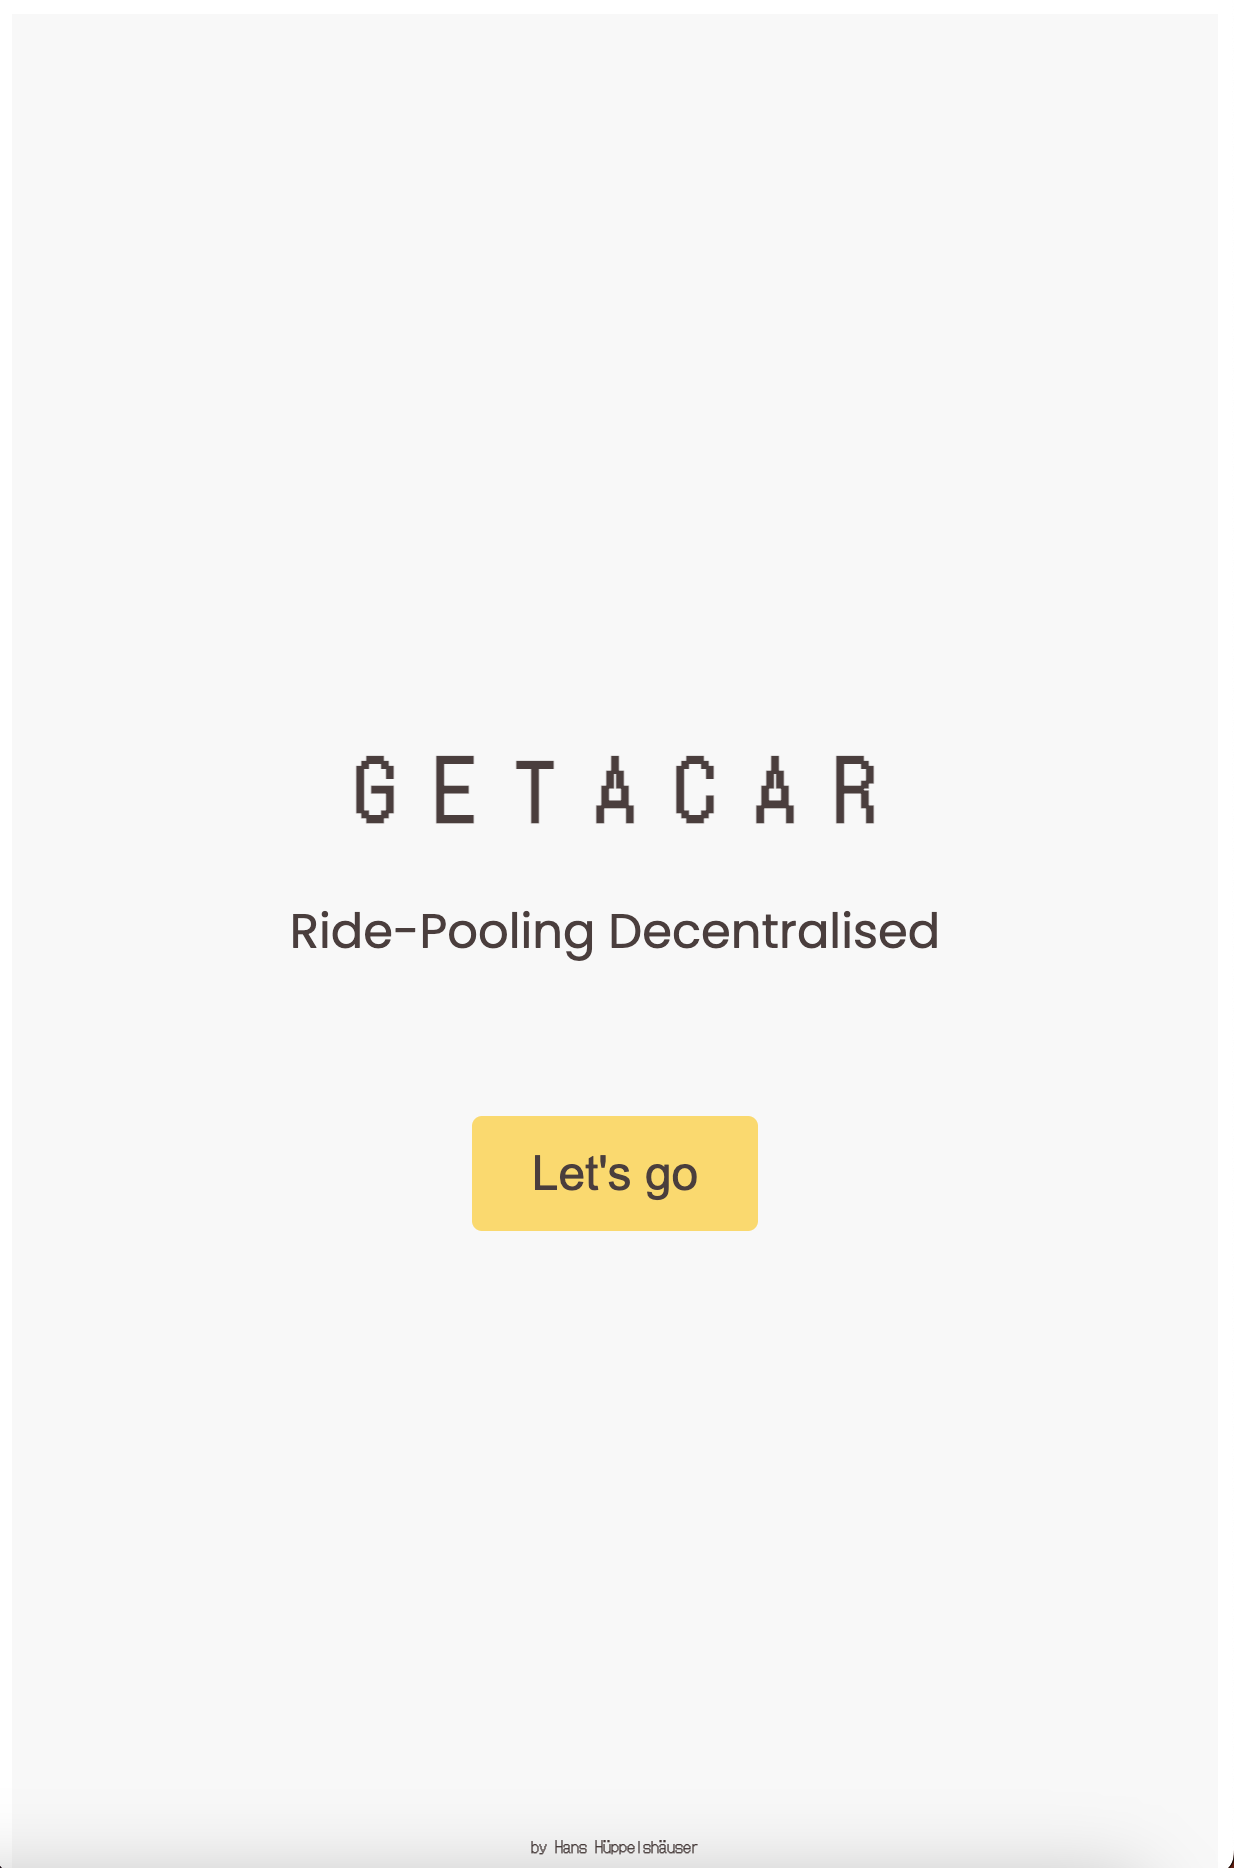
\includegraphics[width=\linewidth]{data/ffss/1.png}
        \caption{Frontend: Welcome Screen}
        \label{fig:WelcomeScreen}
    \end{minipage}
    \hfill
    \begin{minipage}{0.45\linewidth}
        \centering
        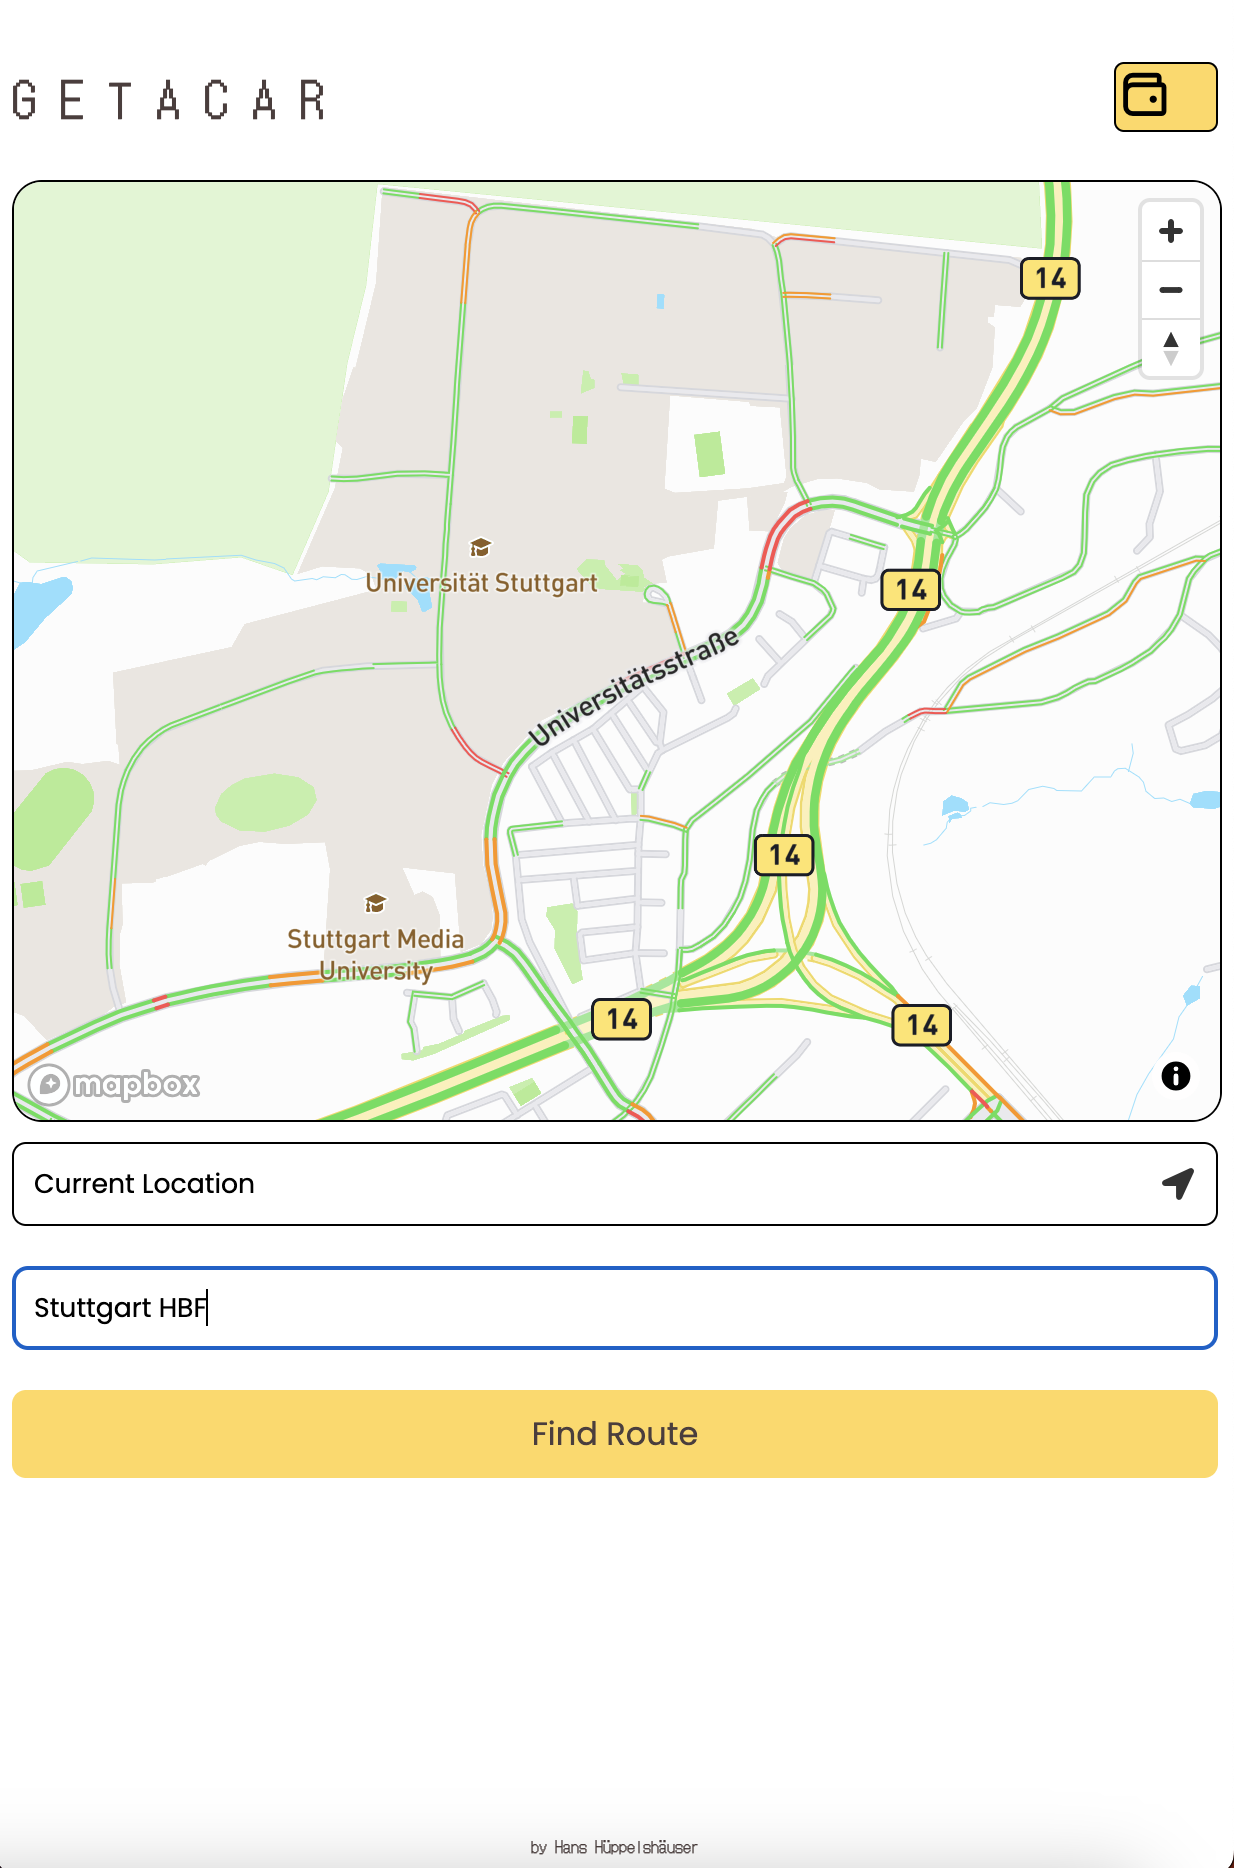
\includegraphics[width=\linewidth]{data/ffss/2.png}
        \caption{Frontend: Map Screen}
        \label{fig:MapScreen}
    \end{minipage}
    
\end{figure}

After the customer presses the ''Find Route'' button they will be presented with the preview of their trip, including some additional information like the expected duration and distance of the travel. The customer has now the possibility to post a ride request by pressing the ''Request Ride'' button, as shown in \ref{fig:MapTripScreen}.
This will send a ride request to the the matching service (that was suggested through the matching smart contract). As long as the auction is running on the matching service the customer frontend will display the loading screen seen in \ref{fig:SearchRideScreen}.


\begin{figure}[H]
    \centering
    
    \begin{minipage}{0.45\linewidth}
        \centering
        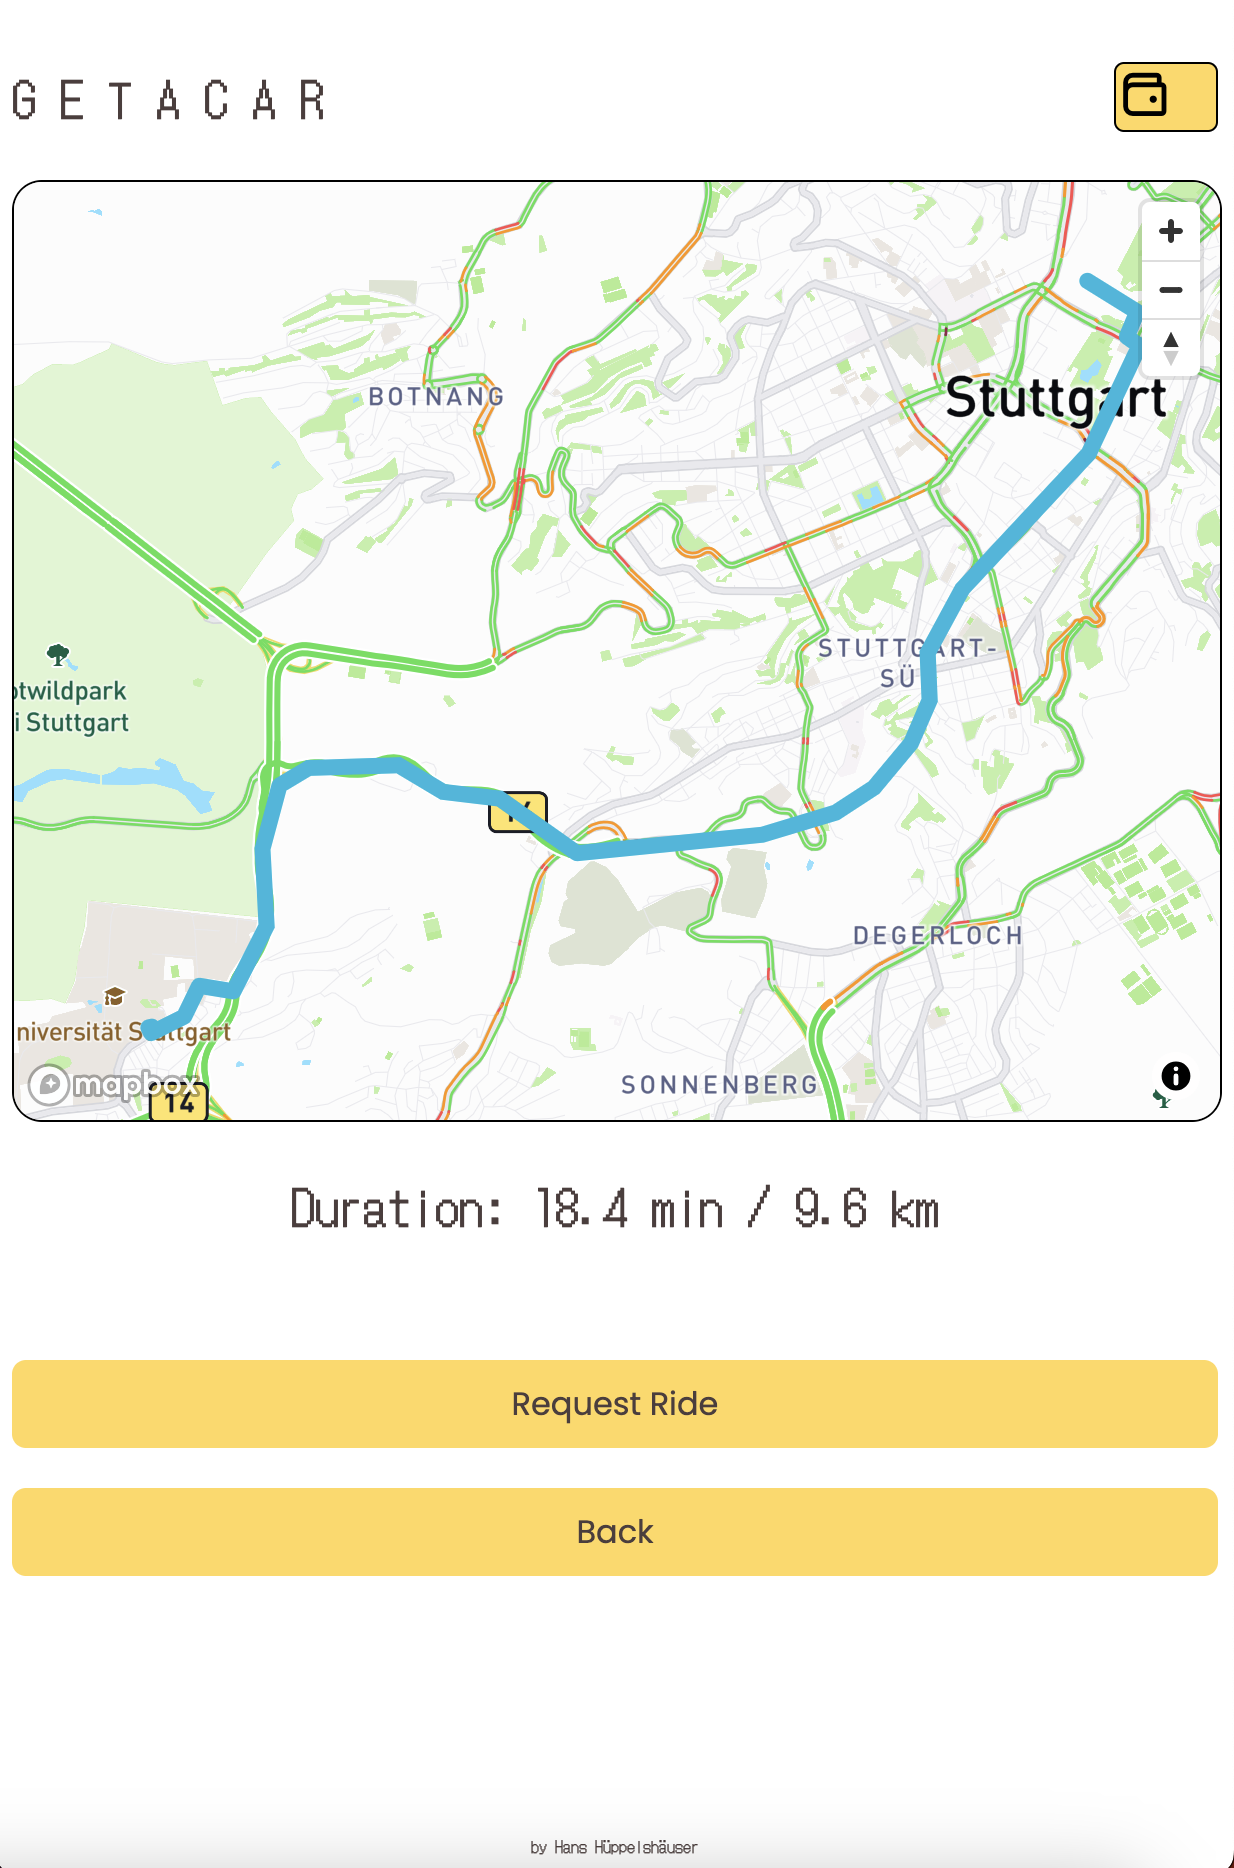
\includegraphics[width=\linewidth]{data/ffss/3.png}
        \caption{Frontend: Map Trip Screen}
        \label{fig:MapTripScreen}
    \end{minipage}
    \hfill
    \begin{minipage}{0.45\linewidth}
        \centering
        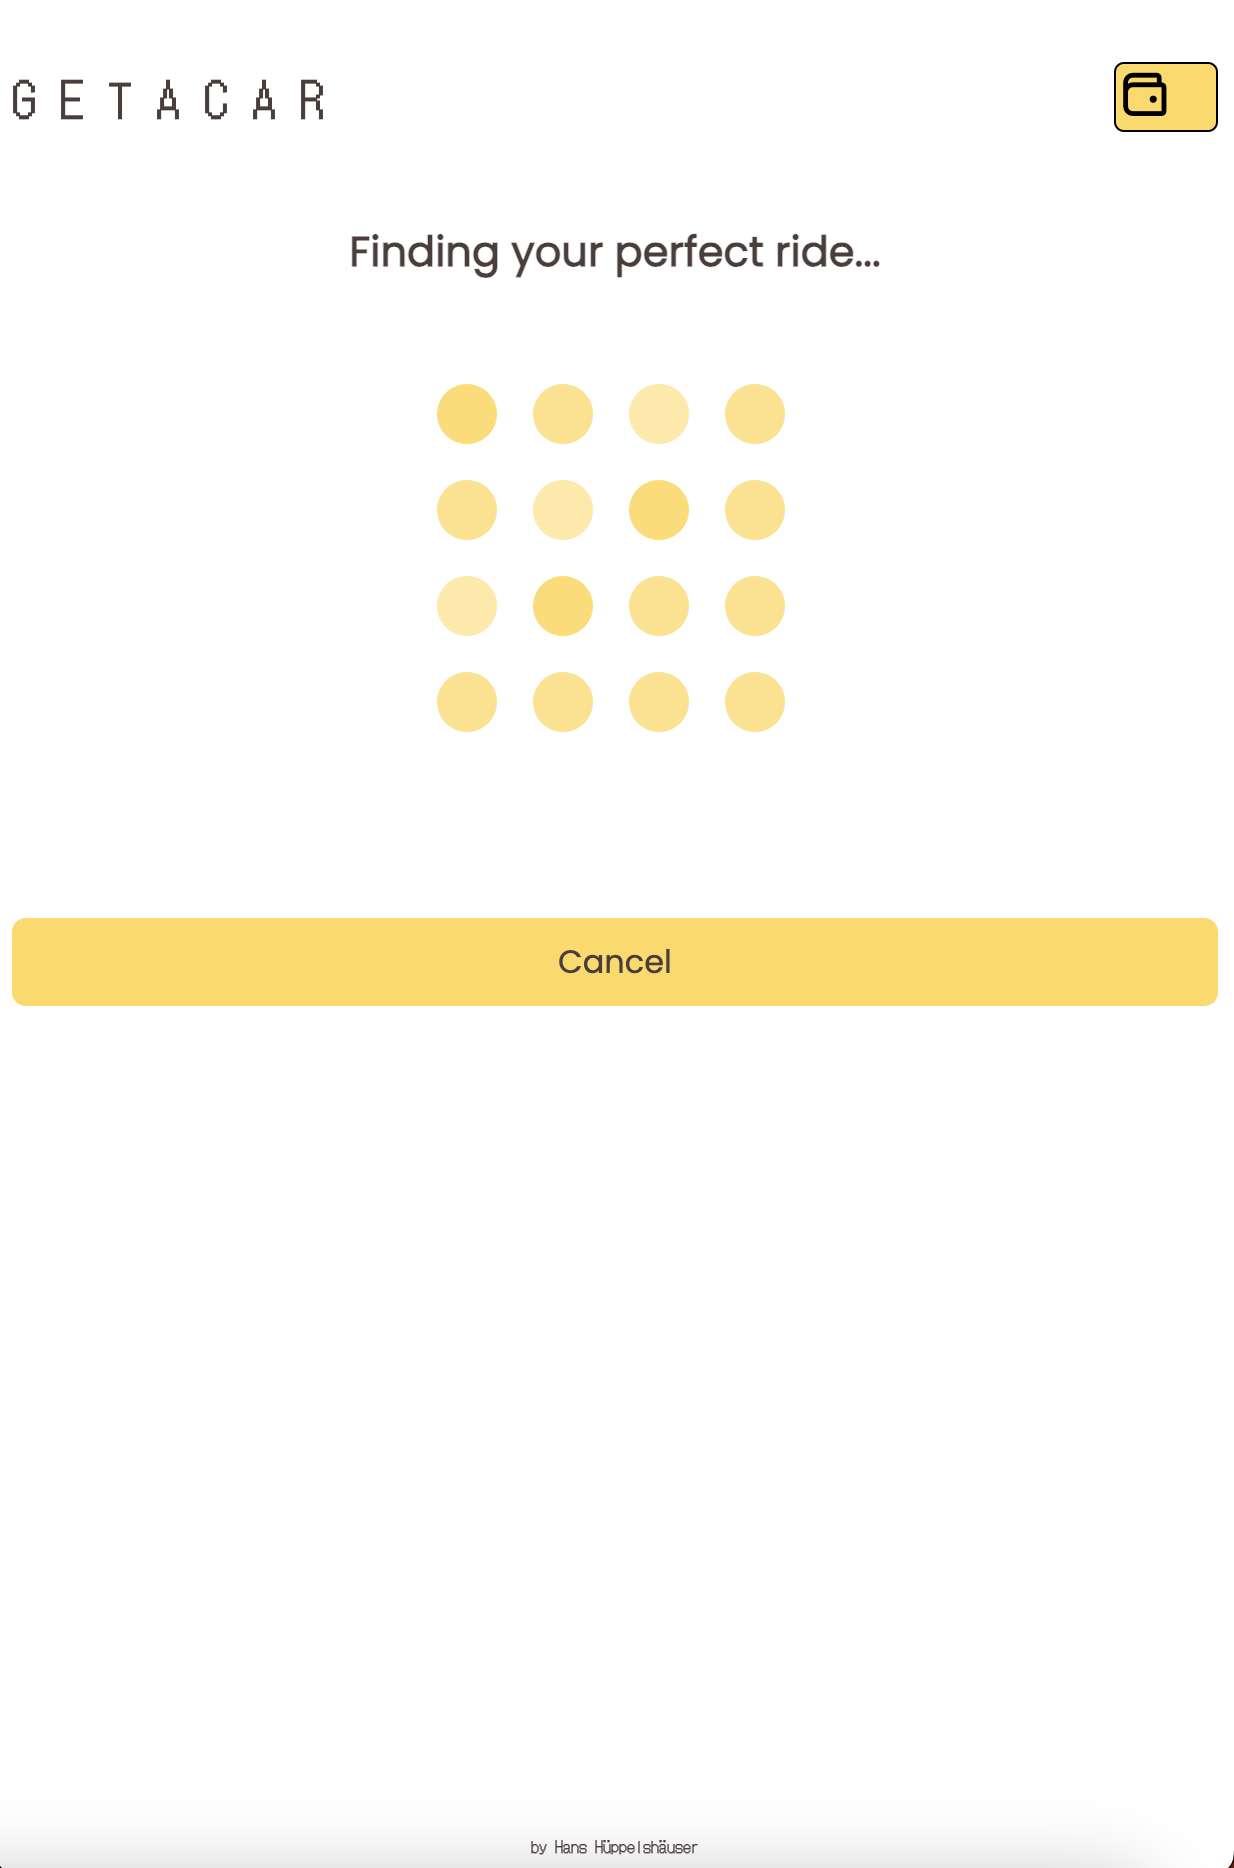
\includegraphics[width=\linewidth]{data/ffss/4.png}
        \caption{Frontend: Search Ride Screen}
        \label{fig:SearchRideScreen}
    \end{minipage}
    
\end{figure}

Once the auction is closed, the customer is presented the winning bid with all the important information about the ride, as shown in \ref{fig:RideOverviewScreen}. In the top right corner a timer counts down the time that is left before the offer expires. As long as the offer has not expired the customer is able to press the ''Book Ride'' button to confirm the ride and thereby create a ride contract on the blockchain. The frontend also has dedicated screens that inform the customer if the matching service could not find a ride or if the offer expiereced because the customer did not press the ''Book Ride'' button.

After a ride is found and the customer confirmed the ride, the frontend changes into the on-ride view that provides status updates about all activities happening on the ride and tracks them via the ride contract. Screen \ref{fig:AwaitingConfirmationScreen} shows the ''waiting Confirmation Screen''. At this stage the frontend monitors the blockchain and waits for the event from the ride contract that signals that the ride provider has co-signed the ride contract.


\begin{figure}[H]
    \centering
    
    \begin{minipage}{0.45\linewidth}
        \centering
        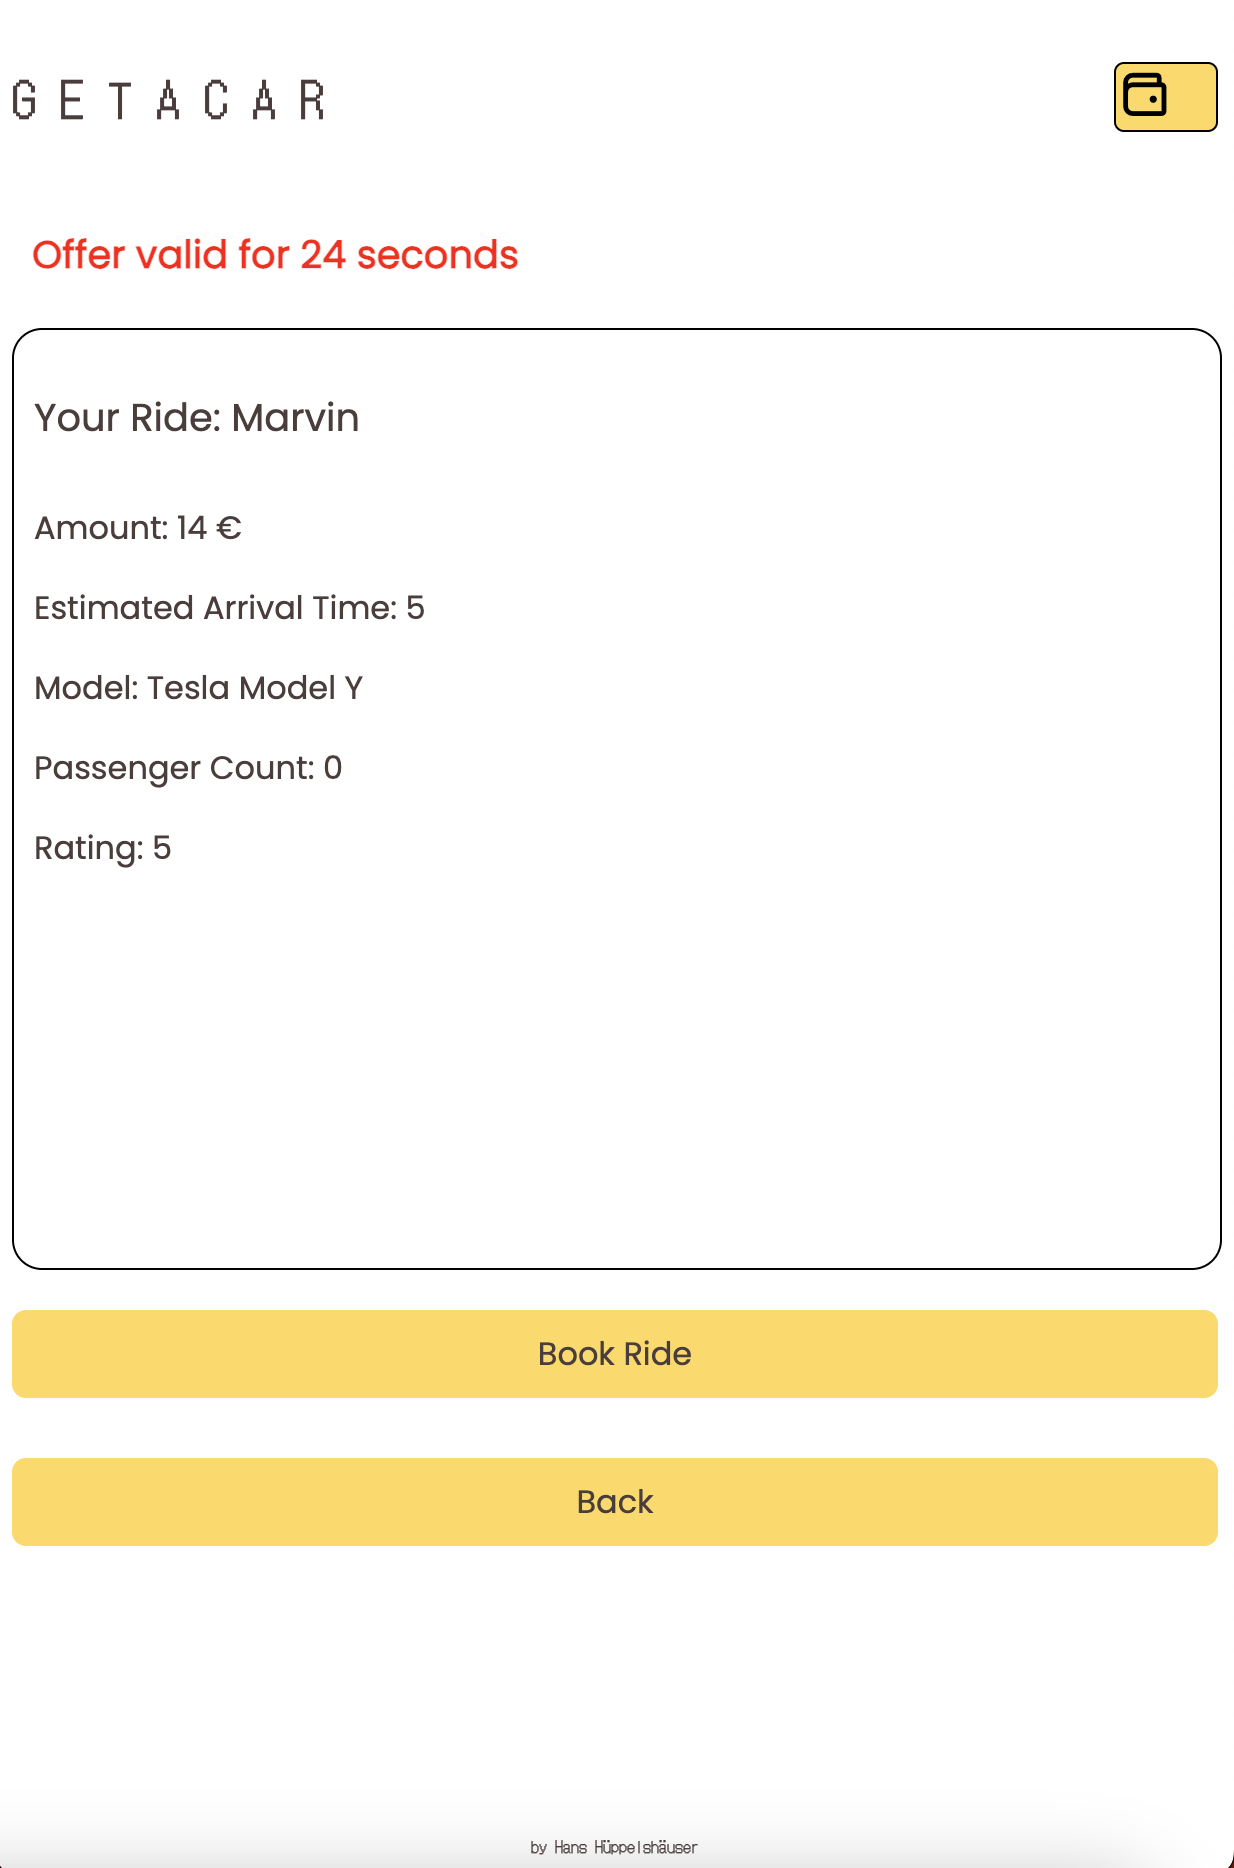
\includegraphics[width=\linewidth]{data/ffss/5.png}
        \caption{Frontend: Ride Overview Screen}
        \label{fig:RideOverviewScreen}
    \end{minipage}
    \hfill
    \begin{minipage}{0.45\linewidth}
        \centering
        
\includegraphics[width=\linewidth]{data/ffss/6.png}
        \caption{Frontend: Awaiting Confirmation Screen}
        \label{fig:AwaitingConfirmationScreen}
    \end{minipage}
    
\end{figure}

When the ride provider has signed the contract and confirmed that they started driving to the agreed pickup location the on-ride screen changes to display the new status of the ride, as seen in \ref{fig:PickupLocationDriveScreen}. A markted ready version of the platform would also show the live position of the ride provider to the customer that the ride provider has shared as an encrypted message through the ride contract. But this feature is not part of the prototype implementation as the prototype only utilises virtual vehicles as ride providers that are not able to provide real-time GPS position updates.

Once the ride provider has arrived at the pickup location and posted this update on the ride contract, the customers frontend changes again to display the update, shown in \ref{fig:VehicleArrivedScreen}. The customer now enters the vehicle and once they are ready to start their ride they confirm this trough the ''Start Driving'' button.


\begin{figure}[H]
    \centering
    
    \begin{minipage}{0.45\linewidth}
        \centering
        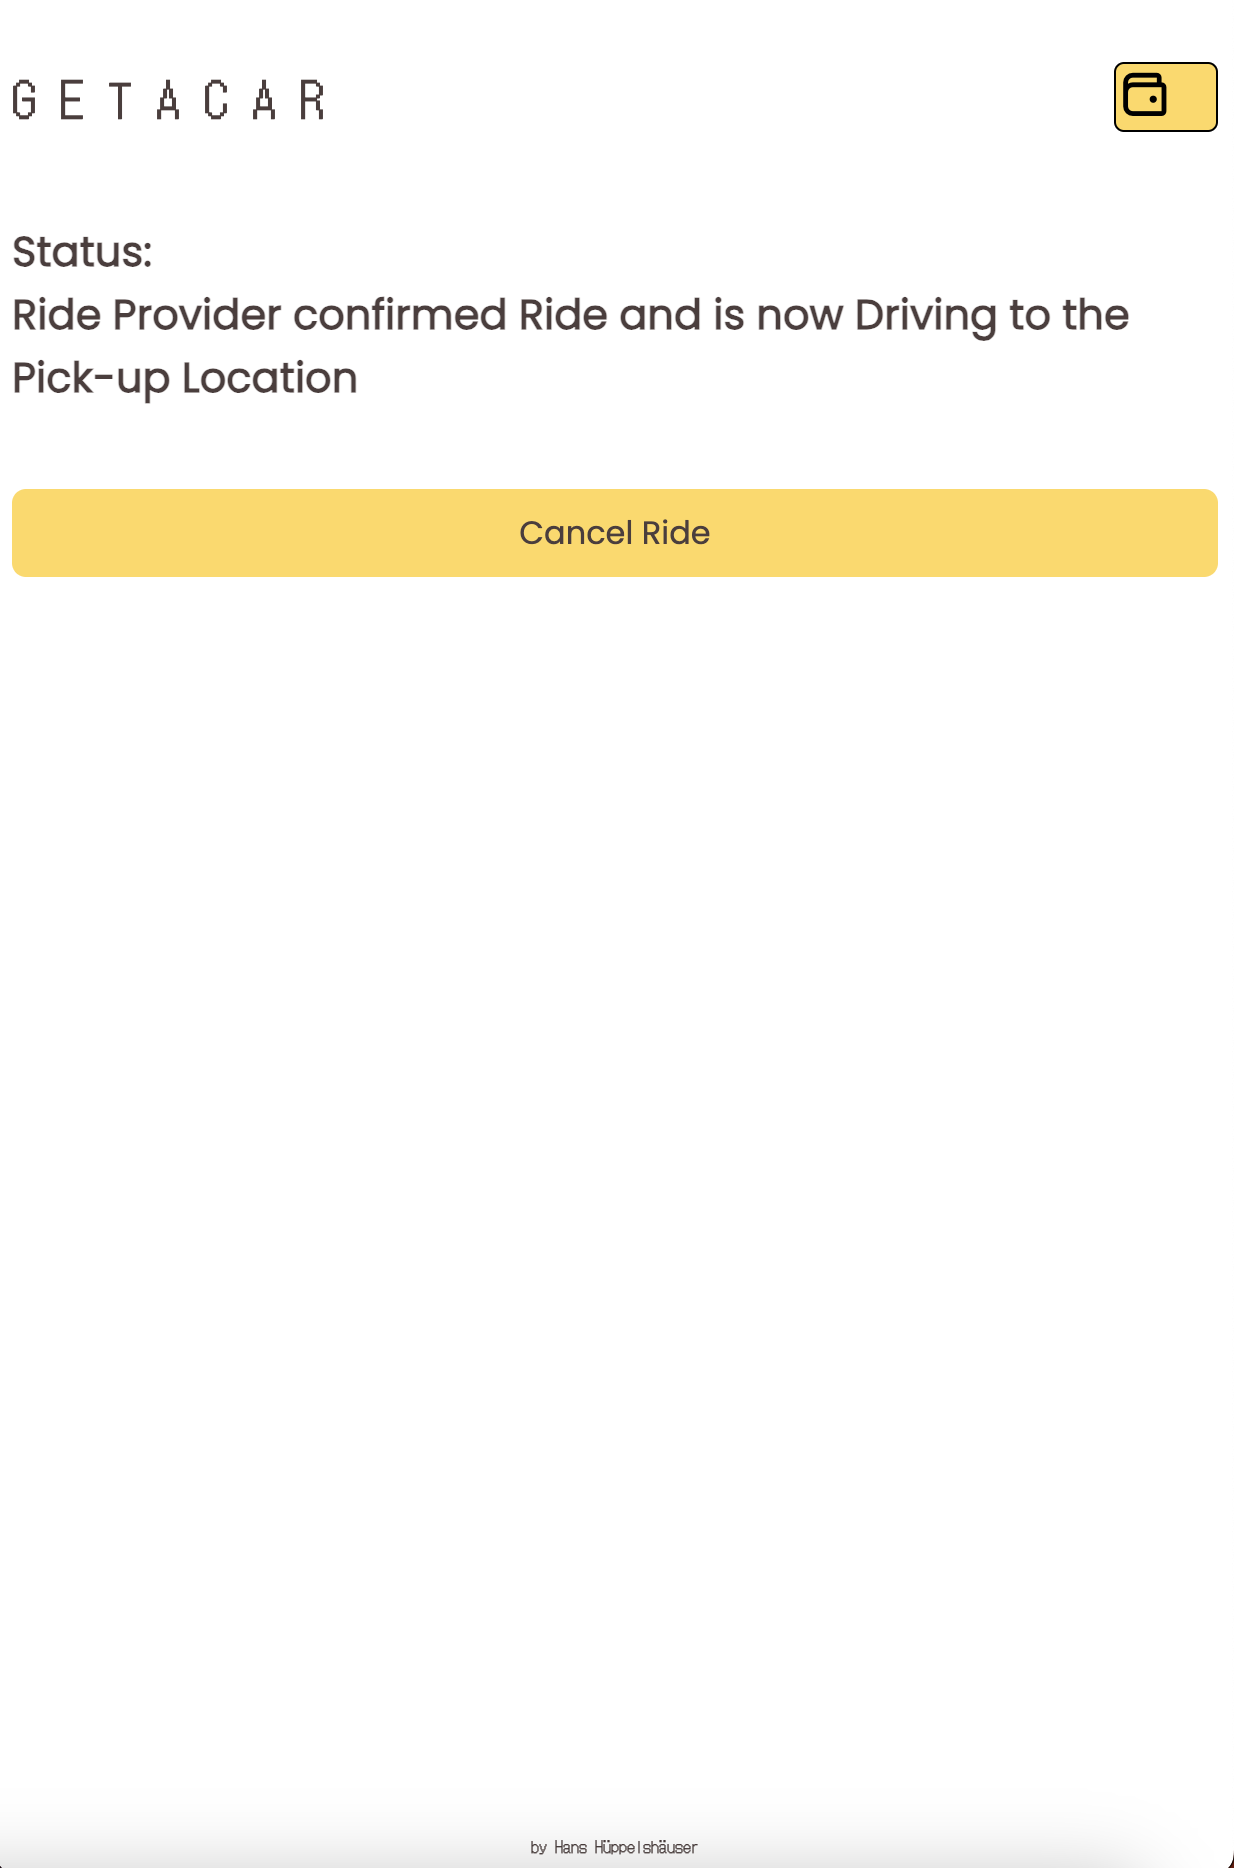
\includegraphics[width=\linewidth]{data/ffss/7.png}
        \caption{Frontend: Pickup Location Drive Screen}
        \label{fig:PickupLocationDriveScreen}
    \end{minipage}
    \hfill
    \begin{minipage}{0.45\linewidth}
        \centering
        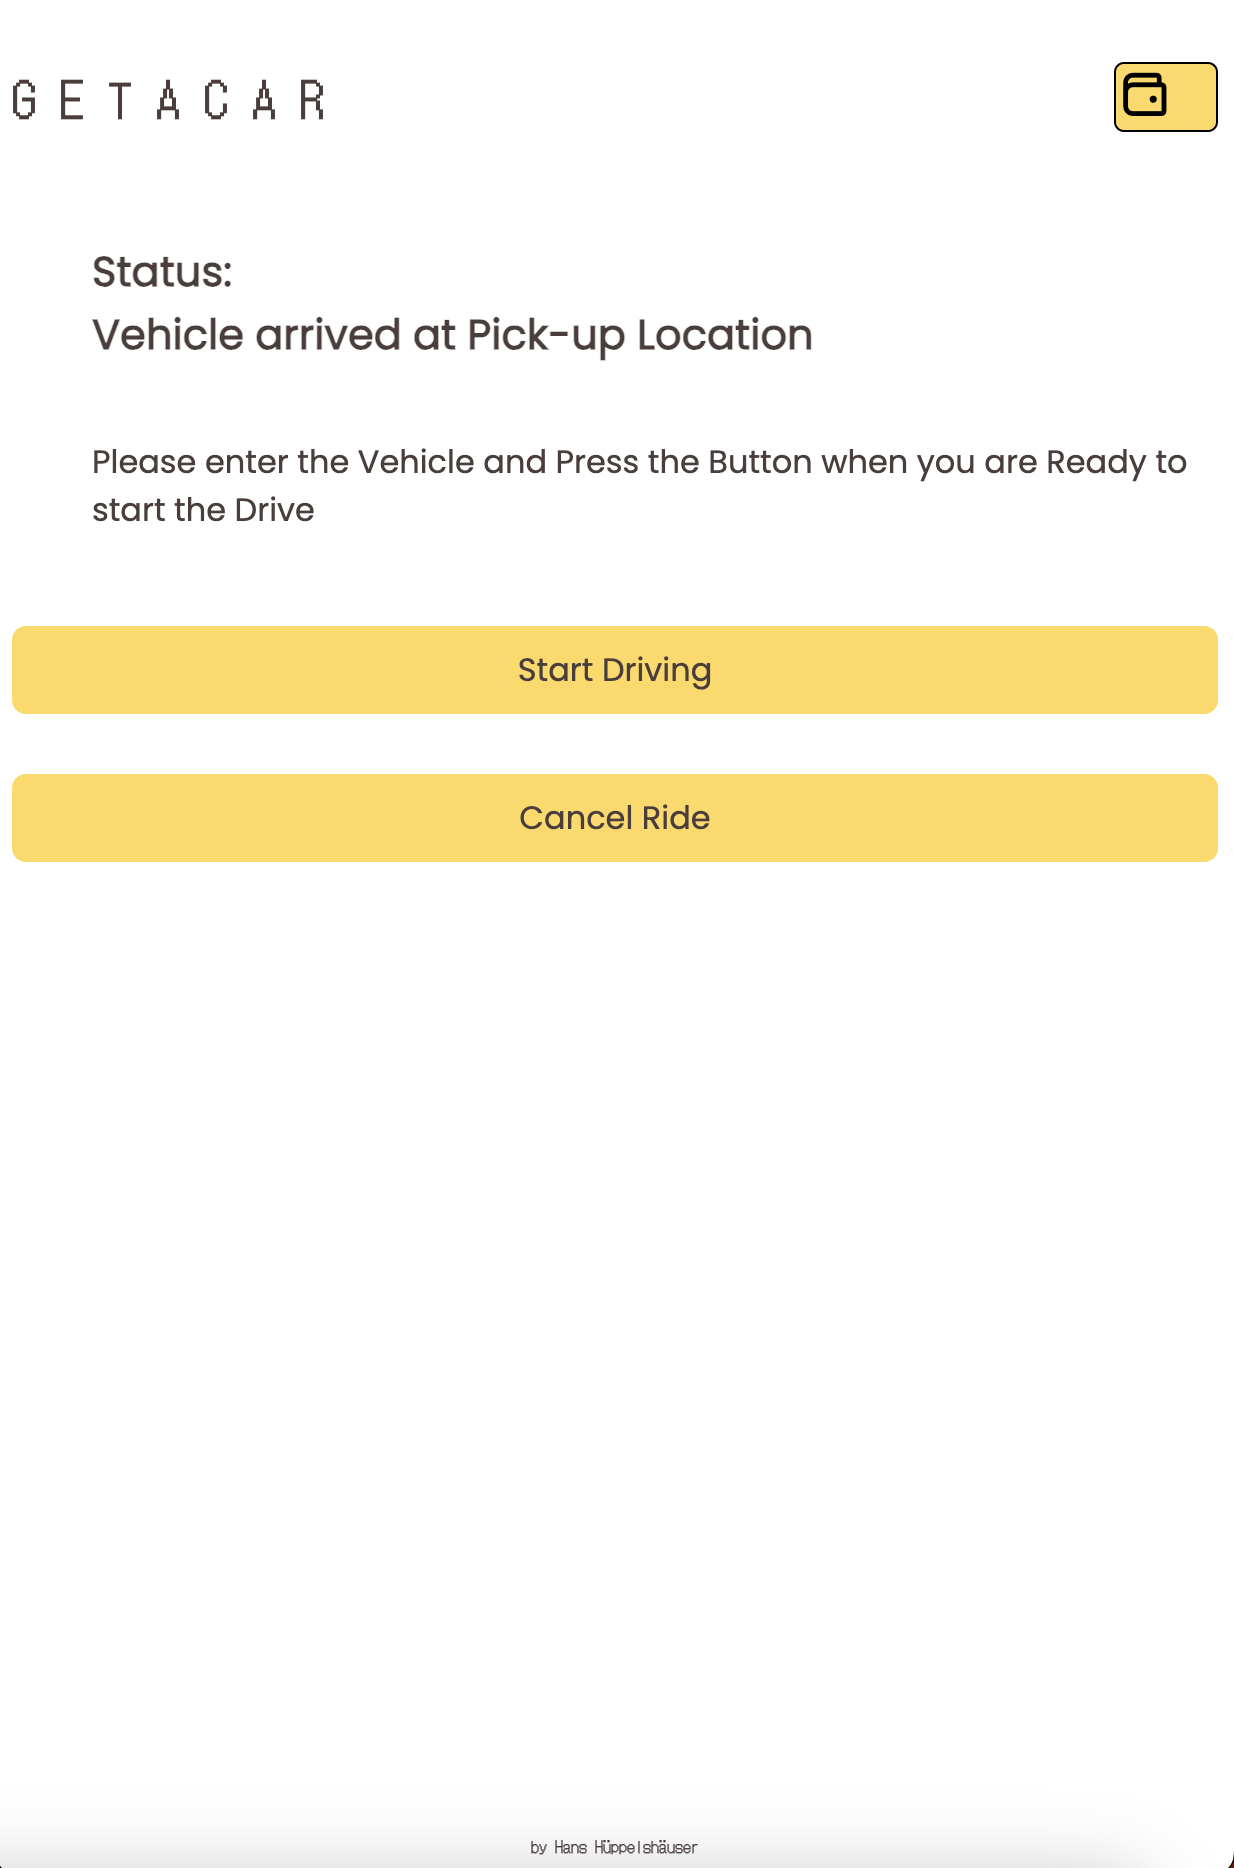
\includegraphics[width=\linewidth]{data/ffss/8.png}
        \caption{Frontend: Vehicle Arrived Screen}
        \label{fig:VehicleArrivedScreen}
    \end{minipage}
    
\end{figure}

After the ride provider has received the update from the customer that they are ready, the ride provider starts the ride to the destination. This is also represented via a status screen in the customer frontend as shown in \ref{fig:DrivingScreen}. When arriving at the dropoff location the ride provider posts this information onto the ride contract. The customer frontend notices this new event on the blockchain and updates the status of the frontend, as seen in \ref{fig:DestinationScreen}. On this screen the customer has the possibility to confirm the ride completion and thereby end the ride process.

It is important to note that each status screen also provides a ''Cancel Ride'' button at all time that allows the customer to aboard the ride process as described in XXX.

\begin{figure}[H]
    \centering
    
    \begin{minipage}{0.45\linewidth}
        \centering
        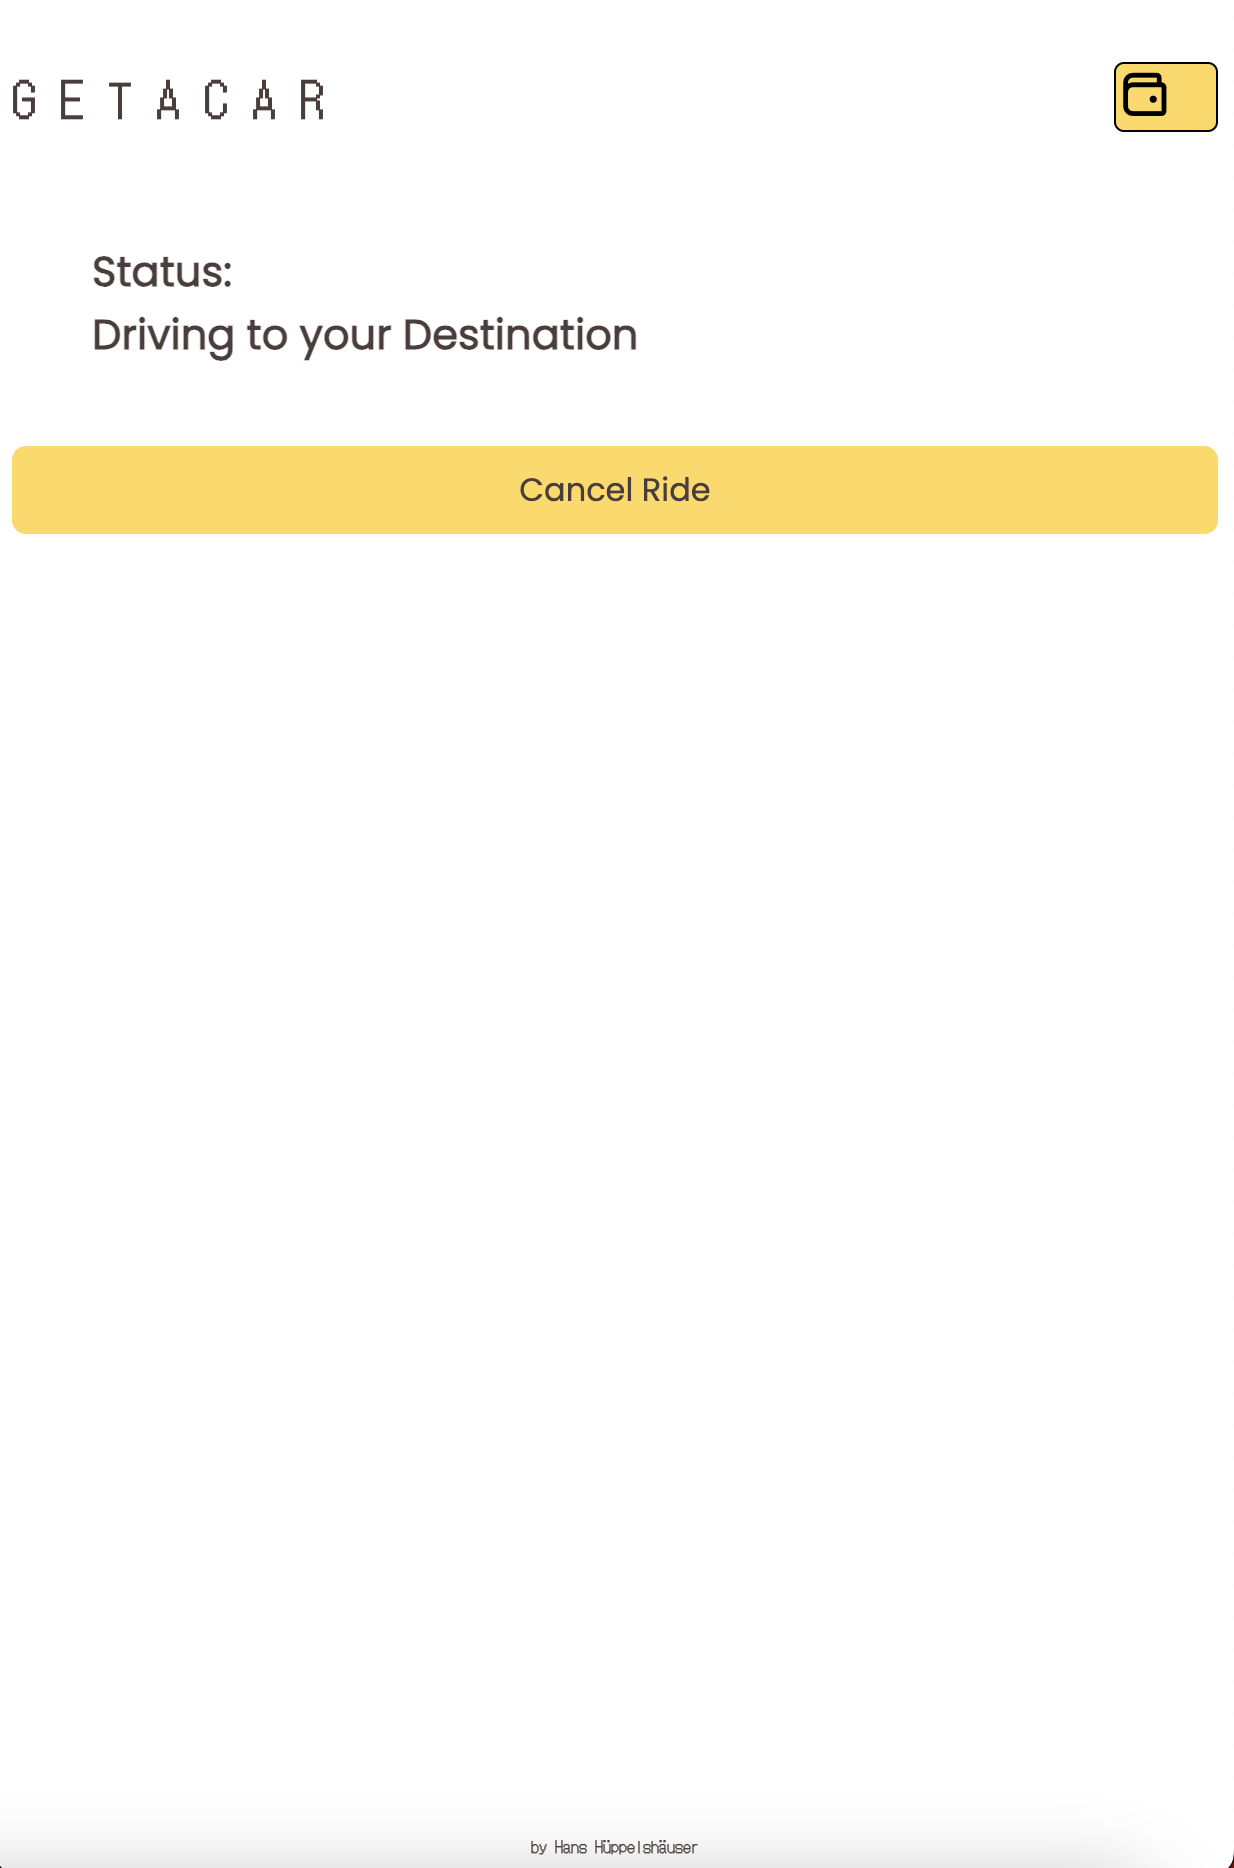
\includegraphics[width=\linewidth]{data/ffss/9.png}
        \caption{Frontend: Driving Screen}
        \label{fig:DrivingScreen}
    \end{minipage}
    \hfill
    \begin{minipage}{0.45\linewidth}
        \centering
        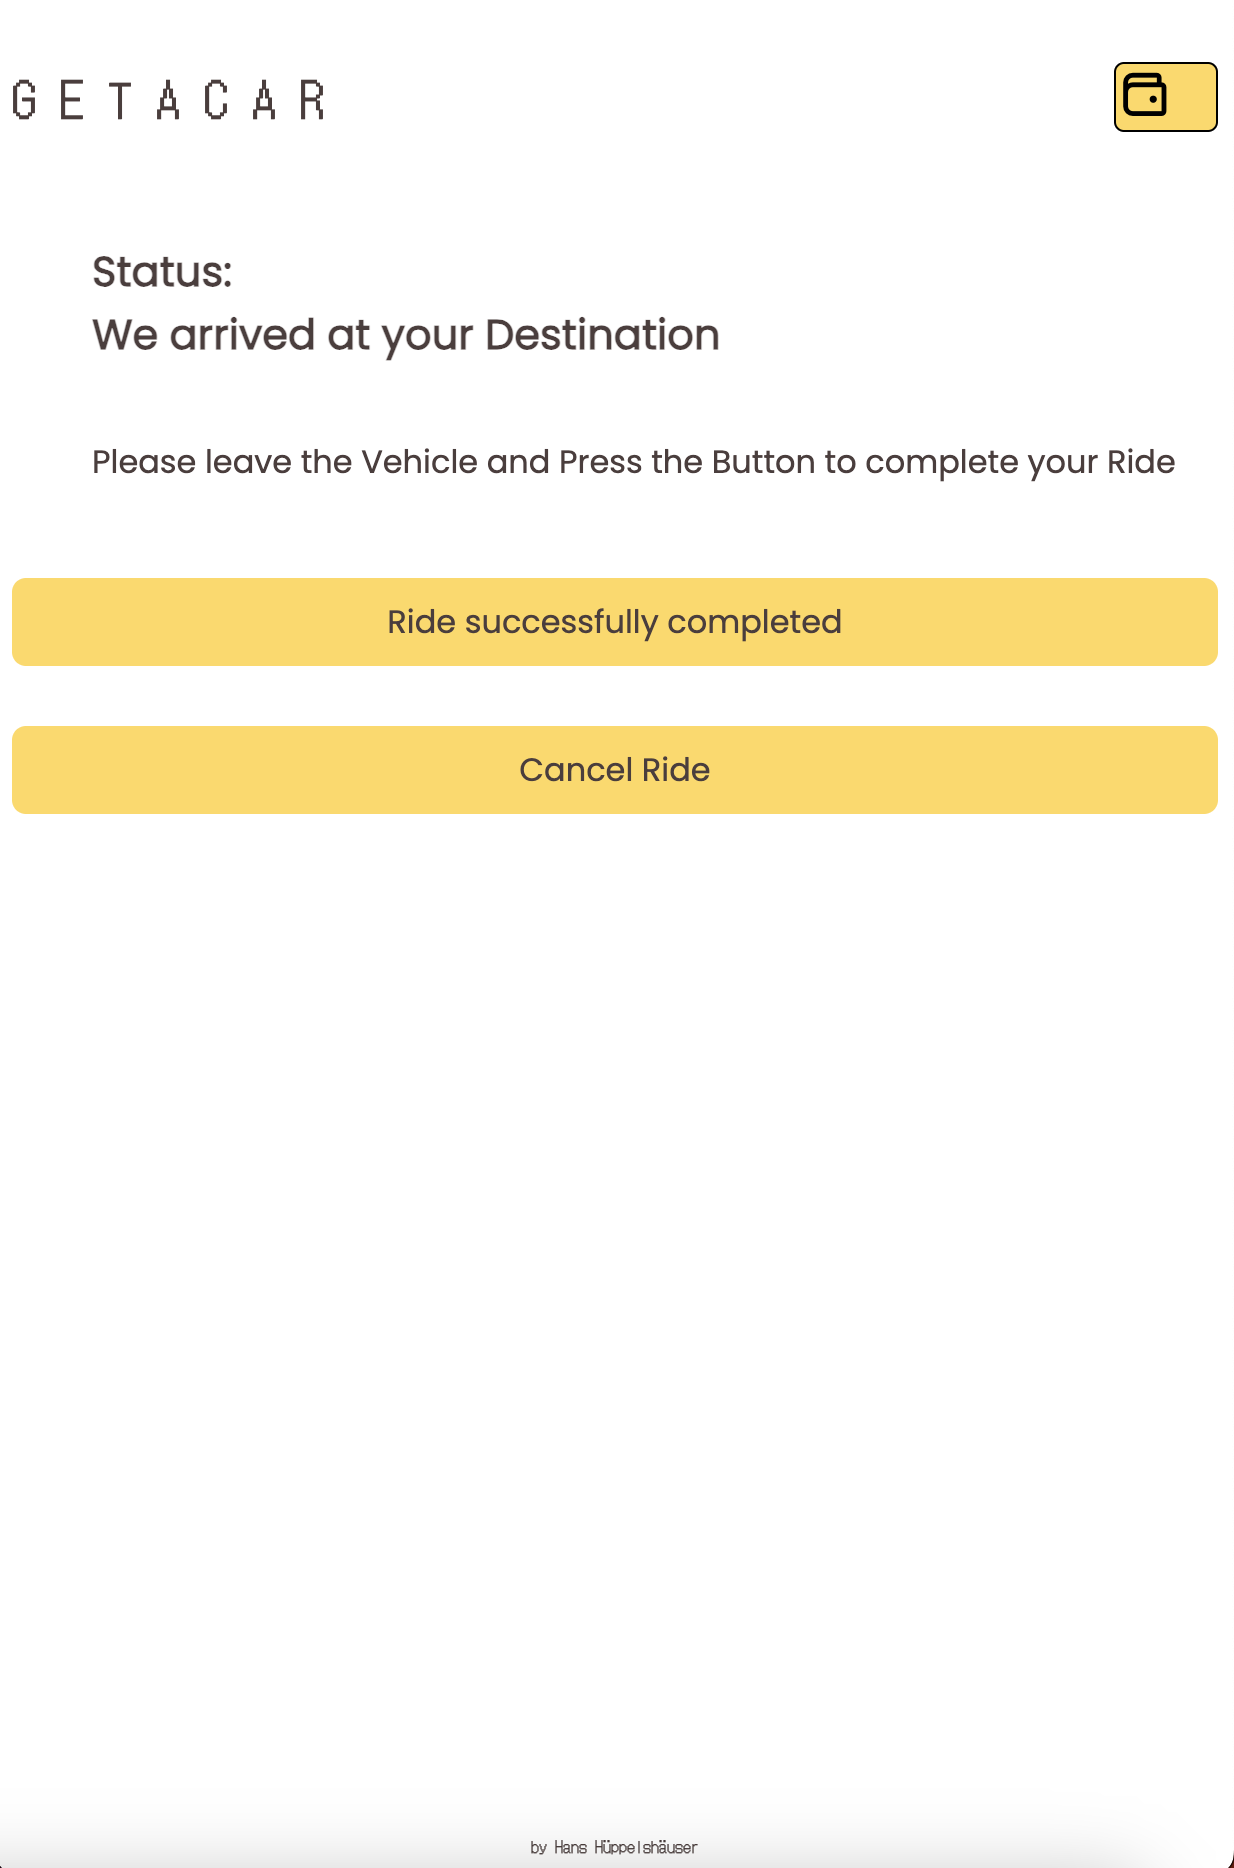
\includegraphics[width=\linewidth]{data/ffss/10.png}
        \caption{Frontend: Destination Screen}
        \label{fig:DestinationScreen}
    \end{minipage}
    
\end{figure}

Once the ride has ended the customer is provided with a ''Ride Completed'' screen that allows the customer to rate the ride provider itself and their passengers, seen in \ref{fig:RateRideProviderScreen}. As described in XXX, the problem with rating passengers is that no personal information should be exchanged through the platform about the passengers. This makes it complicated to ensure that the customer knows who is who when rating multiple passengers. To solve this problem the ride provider shares the seating position and the start time of each passenger with the customer. The seating position is then visualised by the frontend, as seen in \ref{fig:RatePassengerScreen}. In this example passenger that is getting rated was sitting on seat number one, which is the seat on the front row on the left. 



\begin{figure}[H]
    \centering
    
    \begin{minipage}{0.45\linewidth}
        \centering
        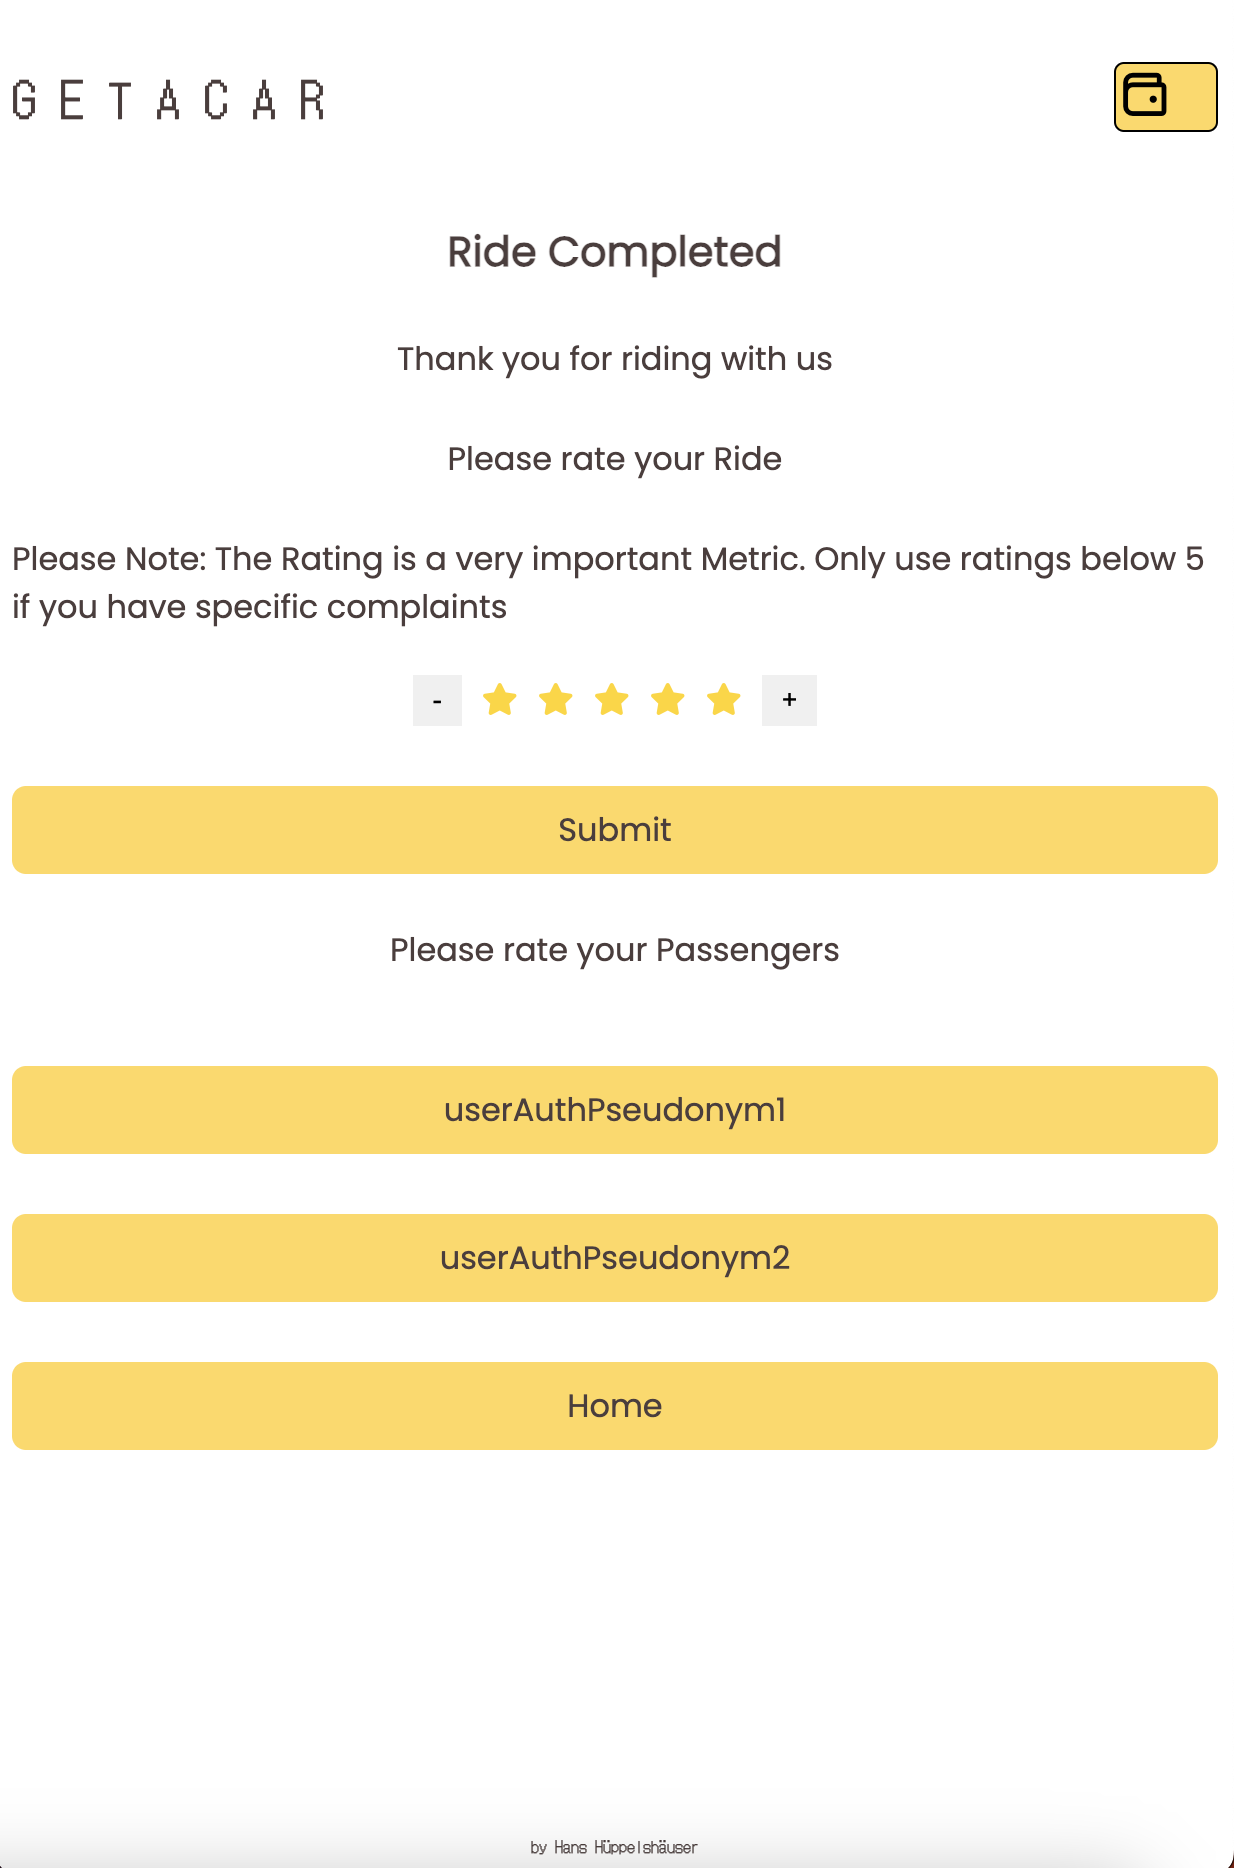
\includegraphics[width=\linewidth]{data/ffss/11.png}
        \caption{Frontend: Rate Ride Provider Screen}
        \label{fig:RateRideProviderScreen}
    \end{minipage}
    \hfill
    \begin{minipage}{0.45\linewidth}
        \centering
        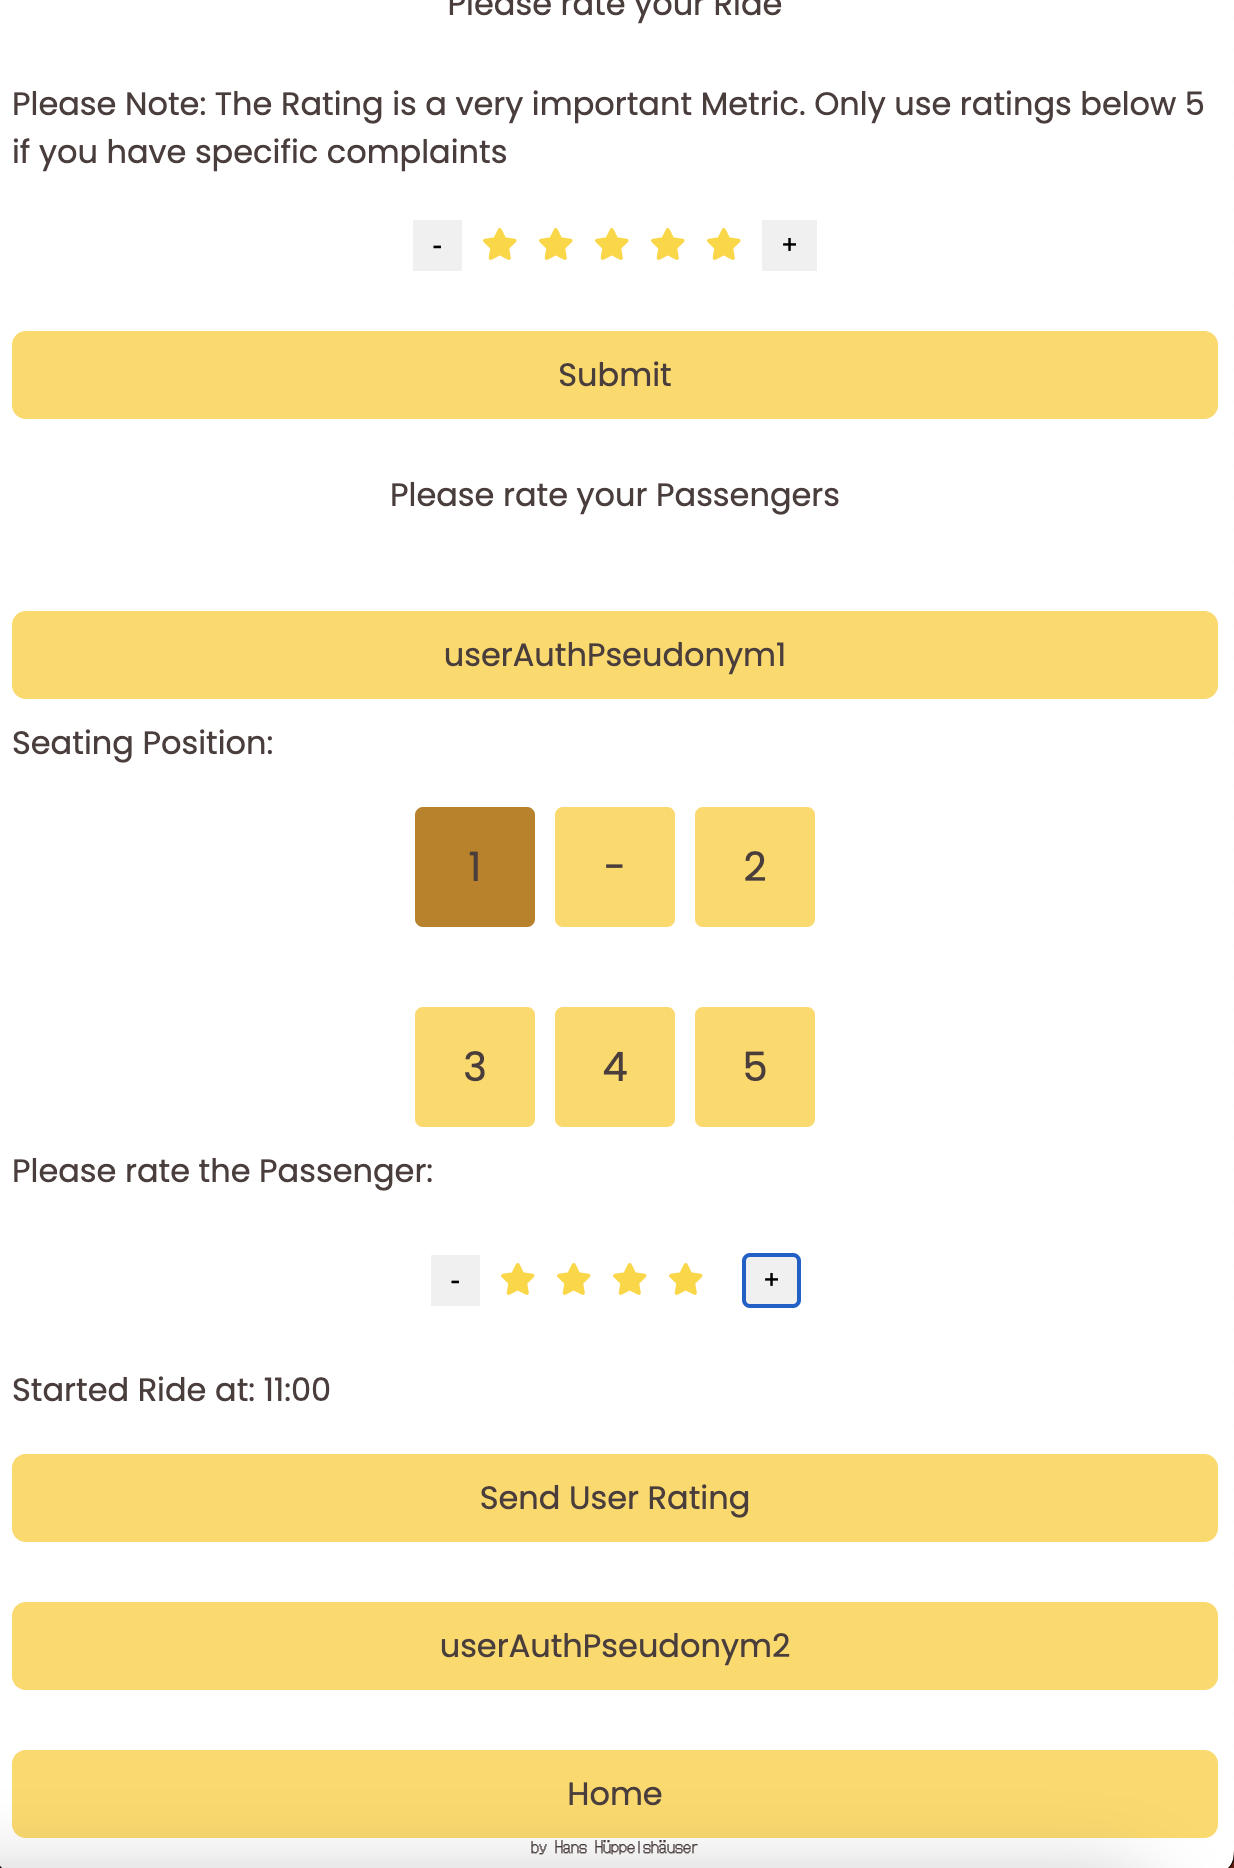
\includegraphics[width=\linewidth]{data/ffss/12.png}
        \caption{Frontend: Rate Passenger Screen}
        \label{fig:RatePassengerScreen}
    \end{minipage}
    
\end{figure}

Last but not least the prototype frontend  also contains the settings view as seen in XXX, that can be opened by pressing the wallet icon in the top right corner of the UI. Here the customer has a number of sliders available to adjust ride booking preferences like the minimum ride provider rating and the maximum amount of passengers that they want to share the ride with at once. This view also shows the rating of the customer them self as well as some additional information like the wallet id that is used to connect to the platform and the account balance of the wallet. These information are only implemented for the prototype as the market ready implementation of the frontend would manage multiple wallets at once. One for each ride. And the wallets would be managed by the frontend in the background as the customer does not has to manage all the wallets by them self and each wallet will only be charged with the amount of money needed for one ride through a crypto exchange.

\begin{figure}[H]
    \centering
    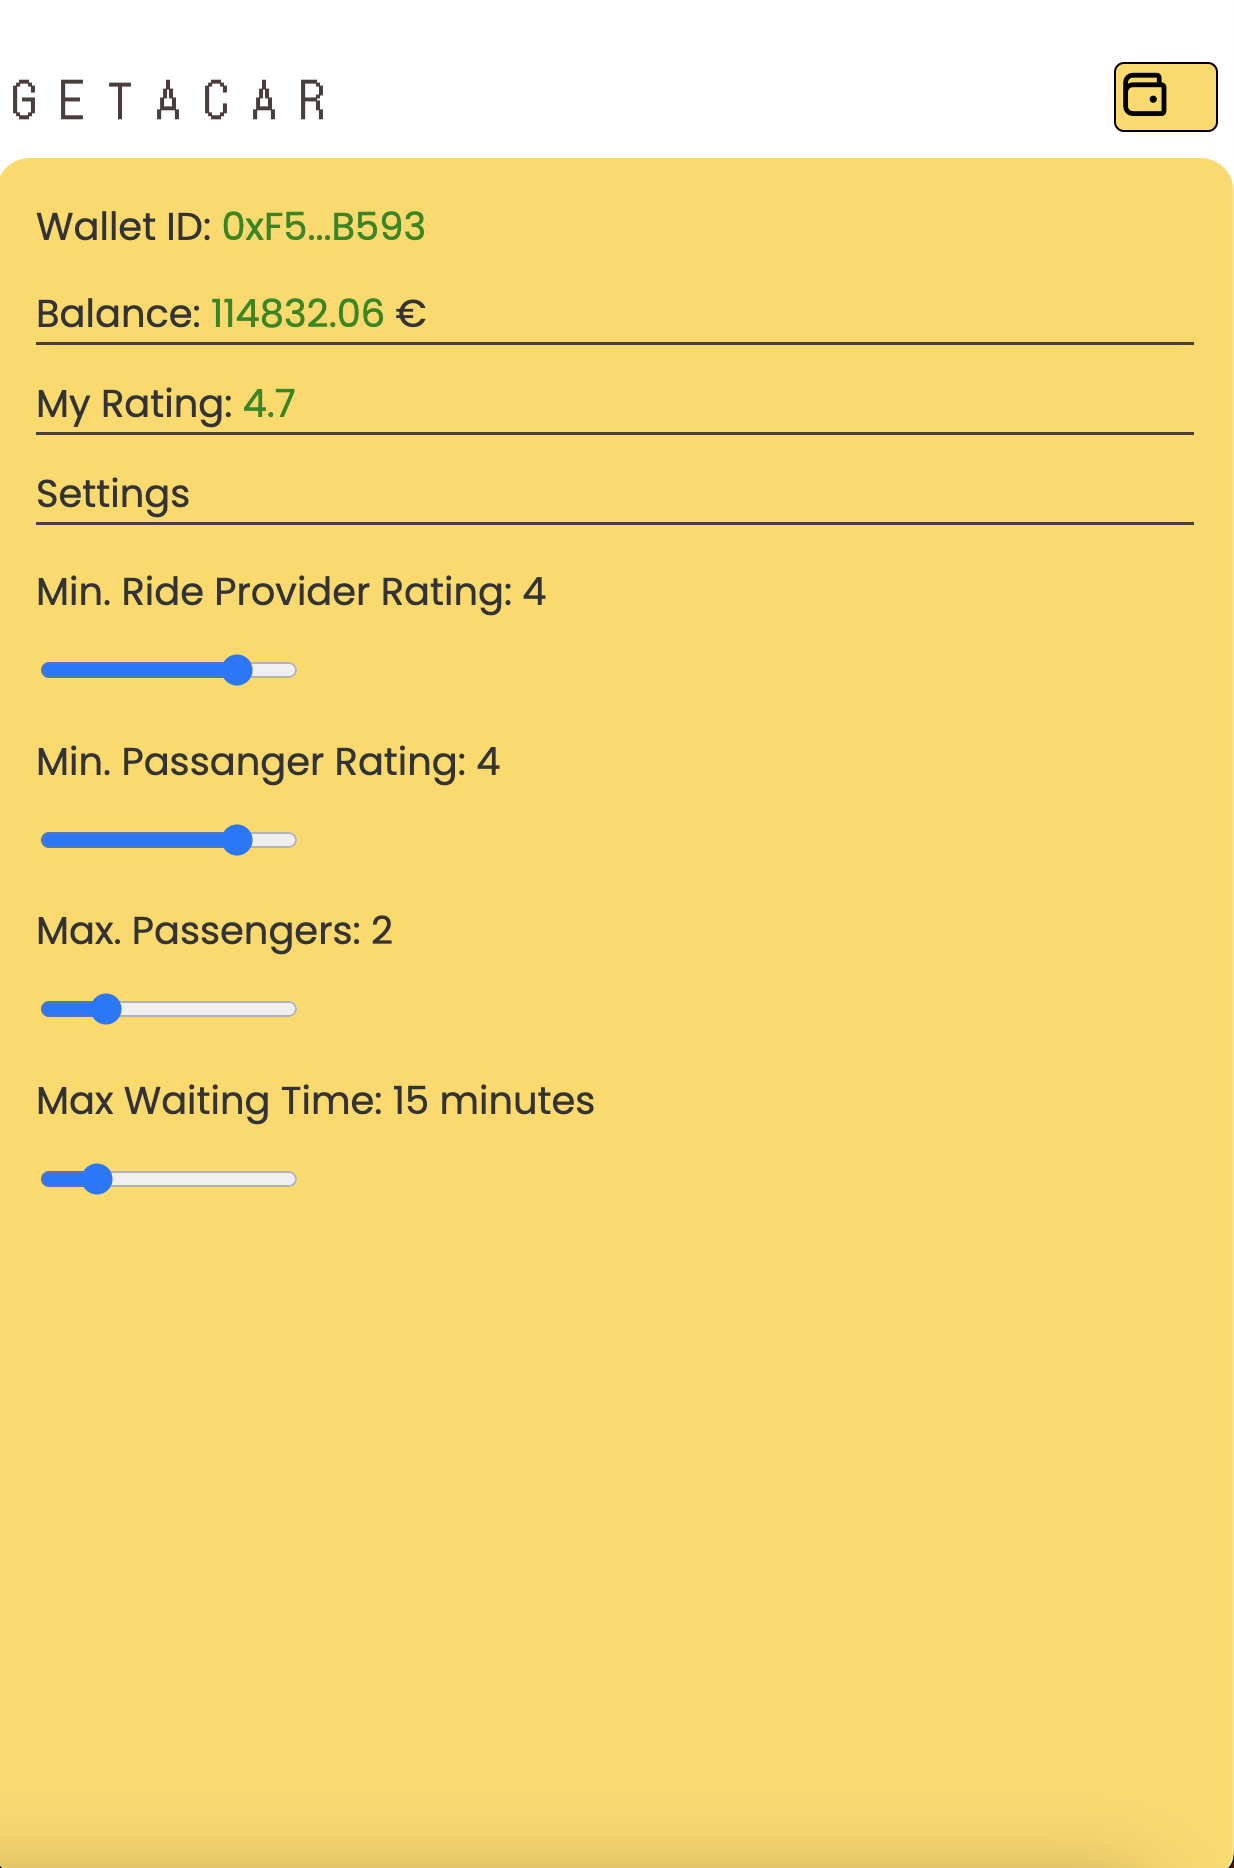
\includegraphics[width=0.45\linewidth]{data/ffss/13.png}
    \caption{Frontend: Settings Screen}
    \label{fig:SettingsScreen}
\end{figure}


\subsection{Customer Frontend Logic}
Now that the user flow of the customer frontend is shown it is important to take a short look at the code logic behind the UI. While most of the logic behind the frontend is standard angular code, the utilisation of the web3 package is notable, as it allows the frontend to directly interact with smart contracts. To demonstrate this interaction the setUserReadyToStartRide() function is chosen as an example. This function gets triggered when a customer presses the ''Start Driving'' button shown in \ref{fig:VehicleArrivedScreen}. First the function checks if a wallet is connected with the frontend. The prototype utilises the external wallet provider MetaMask to manage multiple wallets. After the check was successful the function initiates a new, local instance of the contract. Once this is done successfully the method calls the setUserReadyToStartRide() function inside the ride contract with an encrypted userReadyToStartRideMessage as input, first to calculate the excepted Gas fee and after the transaction is confirmed through Meta Mask by the user, a second time to actually trigger the setUserReadyToStartRide() function inside the ride contract.

\definecolor{verylightgray}{rgb}{.97,.97,.97}

% Define the JavaScript language for lstlisting
\lstdefinelanguage{JavaScript}{
  keywords={typeof, new, true, false, catch, function, return, null, catch, switch, var, if, in, while, do, else, case, break, async, await, const, let, on},
  keywordstyle=\color{blue}\bfseries,
  ndkeywords={class, export, boolean, throw, implements, import, this},
  ndkeywordstyle=\color{darkgray}\bfseries,
  identifierstyle=\color{black},
  sensitive=false,
  comment=[l]{//},
  morecomment=[s]{/*}{*/},
  commentstyle=\color{gray}\ttfamily,
  stringstyle=\color{red}\ttfamily,
  morestring=[b]',
  morestring=[b]"
}

\lstset{
	language=JavaScript, % <-- Change this to JavaScript
	backgroundcolor=\color{verylightgray},
	extendedchars=true,
	basicstyle=\footnotesize\ttfamily,
	showstringspaces=false,
	showspaces=false,
	numbers=left,
	numberstyle=\footnotesize,
	numbersep=9pt,
	tabsize=2,
	breaklines=true,
	showtabs=false,
	captionpos=b
}

\begin{lstlisting}
  async setUserReadyToStartRide(){

    if (!this.web3) {
      console.error('Wallet not connected');
      return;
    }

    const accounts = await this.web3.eth.getAccounts();
    const selectedAddress = accounts[0];

    // Initialize the contract instance
    this.contract = new this.web3.eth.Contract(
      contractAbi as AbiItem[],
      this.rideContractAddress,
    );

    // Call the createContract function
    const gasEstimate = await this.contract.methods
      .setUserReadyToStartRide(userReadyToStartRideMessage)
      .estimateGas({ from: selectedAddress });

    this.contract.methods
      .setUserReadyToStartRide(userReadyToStartRideMessage)
      .send({ from: selectedAddress, gas: gasEstimate })
      .on('transactionHash', (hash: string) => {
        console.log('Transaction hash:', hash);
      })
      .on('receipt', (receipt: any) => {
        console.log('Transaction receipt events:', receipt);
      })

      .on('error', (error: Error) => {
        console.error('Error:', error);
      });
  }
\end{lstlisting}

All functions that are contained within the customer frontend follow this basic flow to interact with the ride contract on the blockchain.


\subsection{Virtual Vehicle}
The Virtual Vehicle represents a new component introduced for the prototype implementation of the GETACAR platform. The Virtual Vehicle is a software daemon that automatically interacts with the platform as a ride provider. The Virtual Vehicle is written in NodeJs and utilises the same web3 package implementation to interact with the blockchain as the customer frontend. It differentiates itself from the customer frontend by not providing a user frontend but by interacting with the platform in an automated way. When starting the Virtual Vehicle it automatically connects to a predefined matching service and begins to scan for open ride requests. Once it has found a ride request it automatically bids a random amount of money to handle the right. If the Virtual Vehicle wins the auction it will sign the ride contract and start to follow the predefined ride flow until the right is completed. Once the ride is completed or in case the Virtual Vehicle does not win the auction, it starts to bid on new ride requests. To test the platform and the matching service it is possible to spin up multiple Virtual Vehicles that all simultaneously interact with the platform. 
In conclusion, the Virtual Vehicles help with simulating platform traffic and testing the prototypical implementation of GETACAR platform by acting as virtual ride providers. 
\section{Matching Service}
After showcasing the implementation of the smart contracts and the customer and ride provider frontend, the last component that is part of the prototype implementation of the GETACAR platform is the Matching Service. The matching service is written in Node.js\footnote{https://nodejs.org/en} and the bids are stored inside MongoDB\footnote{https://www.mongodb.com} as a NoSQL database. The design decision of utilising a NoSQL database in connection with the matching service was made for several reasons. NoSQL databases provide high performance and simplify the storage of the ride requests and ride bids that are stored as simple JSON objects. Lastly, there is also no need for complex SQL functions inside the matching service that would promote the usage of an SQL database.


\subsection{Endpoints and Data}
The NodeJs application provides four core endpoints for customers and ride providers to handle all interactions with the matching service. Following ride flow, the first endpoint that is typically utilised is the POST /requestRide endpoint. The customer frontend utilises this endpoint to post ride requests to the matching service. The request contains the following data points:

\begin{itemize}
    \item \textbf{userId:} The customer pseudonym provided by an authentication service
    \item \textbf{pickupLocation:} The cloaked pickup location
    \item \textbf{dropoffLocation:} A cloaked dropoff location
    \item \textbf{userRating:} The rating of the customer
    \item \textbf{rating:} The rating of the customer requesting the ride
    \item \textbf{userPublicKey:} A newly generated public key from the customer used for the Diffie-Hellman Key Exchange
    \item \textbf{maxWaitingTime:} The maximum time the customer is willing to wait for the arrival of the ride provider
    \item \textbf{minRating:} The minimum rating necessary for a ride provider to have to be allowed to manage the ride
    \item \textbf{minPassengerRating:} The minimum rating for passengers to have to be allowed to share the ride with the customer
    \item \textbf{maxPassengers:} The maximum amount of passengers the customer is willing to have at once
\end{itemize}

The Matching Service adds the following data points to the ride request and writes them onto the database:

\begin{itemize}
    \item \textbf{rideRequestId:} A unique id to identify the ride request
    \item \textbf{gridLocation:} The grid square from where the ride request came from. This makes it easier for ride provider to find fitting ride requests if a matching service is deployed for a number of different grid squares. 
    \item \textbf{auctionStartedTimestamp:} The timestamp represents the moment the data was posted onto the matching service visibale for ride providers to bid on the ride request. 
    \item \textbf{auctionStatus:} The status of the auction. The auction can have one of four different statuses: 'open', 'determining-winner', 'waiting-for-signature' or 'closed'. 
    \item \textbf{auctionWinner:} The winner of the auction. If the winner was not determined yet, this field is empty.
    \item \textbf{winningBid:} The unique identifier of the winning bid. If the winner was not determined yet, this field is empty.
    \item \textbf{p:} The prime number used for Diffie-Hellman key exchange.
    \item \textbf{g:} The base used for Diffie-Hellman key exchange.
\end{itemize}

Once the complete ride request is available in the database, it can be read by ride providers. Ride providers can use the GET /rideRequests endpoint to receive a JSON object containing all ride requests with open auctions. The ride provider can search this dataset and, once they find a fitting ride request, bid on it.
To bid on a ride request, the ride provider can utilise the POST /bid endpoint. A bid request contains the following data points:

\begin{itemize}
    \item \textbf{rideRequestId:} The id of the ride request that this bid is for
    \item \textbf{rideProviderId:} The ride provider pseudonym provided by an authentication service
    \item \textbf{amount:} The maximum ride cost that the ride provider is willing to offer the ride for
    \item \textbf{rating:} The rating of the ride provider
    \item \textbf{model:} The model of the vehicle
    \item \textbf{estimatedArrivalTime:} The time to get to the customer pickup location
    \item \textbf{passengerCount:} The amount of passengers inside the vehicle when arriving at the pickup location
    \item \textbf{vehiclePublicKey:} A newly generated public key from the ride provider used for the Diffie-Hellman Key Exchange 
\end{itemize}

Before a bid can be posted to the database, the Matching Service compares the timestamp of the bid with the timestamp of the ride request the bid is associated with to ensure that the auction is truly open. For this prototype, the time frame for this is set to 30 seconds. The bid also gets extended with additional data points by the matching service itself before it gets written onto the database. These are the additional data points:

\begin{itemize}
    \item \textbf{bidId:} A unique id to identify the bid
    \item \textbf{bidPlacedTimestamp:} Timestamp representing the moment the bid is posted
\end{itemize}

With ride requests and associated bids being written to the database, the next step for the matching service is handling the running auction. Each auction is posted with the status ''open''. A function managed by the Matching Service continuously crawls the database for ride requests where the auction is older than 30 seconds. If such an auction is found, the auction status changes from 'open' to 'determining-winner'. A second function then takes the ride request and analyses all bids connected with the request to determine the winning bid based on the principles of the second price auction. The winning bid is then written into the ride request itself, changing the auction status to 'waiting-for-signature'. 

The customer is able to check the status of their auction through the GET /rideRequest/:rideRequestId endpoint by providing the identifier of their ride request inside the URL. This endpoint returns the status of the auction, and in case a winning bid is found, it additionally returns the winning bid itself. Based on the winning bid, the customer can then decide if they want to take the ride or not. If the customer decides to take the ride, they follow the ride flow and create a ride contract through the contract factory that contains the maximum ride cost as a deposit. They then need to use the GET setContractAddress/:rideRequestId/:contractAddress endpoint to update their ride request with the contact's address on the blockchain. As the creation of the contract is understood as the initial signing of the ride contract, the status of the auction changes from 'waiting-for-signature' to 'closed'. 

The GET /rideRequest/:rideRequestId endpoint also enables the ride provider to track the status of the auction. Through the endpoint, the auction winner is able to receive the address of the ride contract and is, therefore, able to co-sign the contract as a ride provider.

\subsection{Grid System}
As described in \ref{subsec:MatchingService}, the design of the Matching Service includes a map grid that is utilised to assign matching services to specific jurisdiction zones and to cloak the exact pickup and dropoff locations of customers. There are many possible ways to create a map grid that would allow for this use case. The GETACAR prototype implementation uses H3\footnote{https://h3geo.org}, a hexagonal hierarchical geospatial indexing system that provides a predefined grid for the platform to use. The advantage of H3 is that it provides a number of grid resolutions, as each grid is made up of hexagons and pentagons that themself are made up of smaller hexagons and pentagons. An algorithm allows one to easily check if a hexagon/ pentagon of a smaller resolution is contained within a hexagon/ pentagon of a higher resolution. This approach would allow GETACAR to utilise dynamic resolutions for the  jurisdiction zones and the location cloaking with higher resolutions used for crowded areas with high traffic, like cities and lower resolutions that cover larger, less crowded  areas with less traffic. The prototype uses fixed resolutions with Res 9 for the location cloaking and Res 6 for the  jurisdiction zones of the matching services. 

\begin{figure}[h]
    \centering
    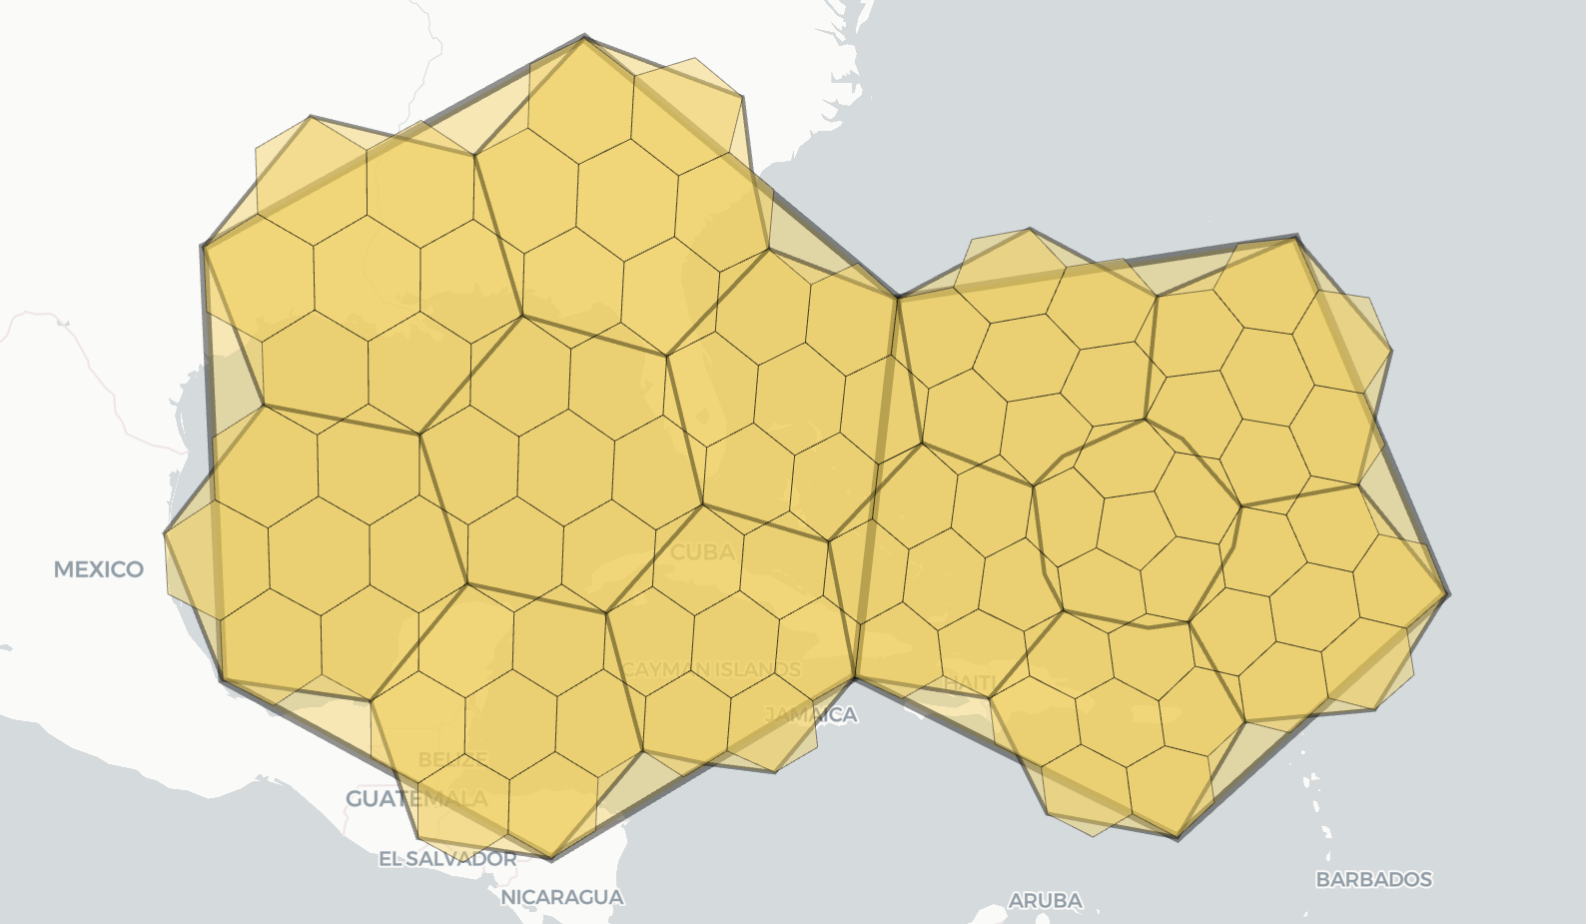
\includegraphics[width=\linewidth]{data/11.png}
    \caption{H3 Grid Visualisation ~\cite{H3Geo.}}
    \label{fig:H3Visualisation}
\end{figure}

\begin{table}[h]
\centering
\begin{tabular}{|c|r|r|r|}
\hline
\textbf{Res} & \textbf{Average Hexagon Area (km$^2$)} & \textbf{Pentagon Area (km$^2$)} & \textbf{Ratio (P/H)} \\
\hline
0 & 4,357,449.416078381 & 2,562,182.162955496 & 0.5880 \\
1 & 609,788.441794133 & 328,434.586246469 & 0.5386 \\
2 & 86,801.780398997 & 44,930.898497879 & 0.5176 \\
3 & 12,393.434655088 & 6,315.472267516 & 0.5096 \\
4 & 1,770.347654491 & 896.582383141 & 0.5064 \\
5 & 252.903858182 & 127.785583023 & 0.5053 \\
6 & 36.129062164 & 18.238749548 & 0.5048 \\
7 & 5.161293360 & 2.604669397 & 0.5047 \\
8 & 0.737327598 & 0.372048038 & 0.5046 \\
9 & 0.105332513 & 0.053147195 & 0.5046 \\
10 & 0.015047502 & 0.007592318 & 0.5046 \\
11 & 0.002149643 & 0.001084609 & 0.5046 \\
12 & 0.000307092 & 0.000154944 & 0.5046 \\
13 & 0.000043870 & 0.000022135 & 0.5046 \\
14 & 0.000006267 & 0.000003162 & 0.5046 \\
15 & 0.000000895 & 0.000000452 & 0.5046 \\
\hline
\end{tabular}
\caption{H3 Grid Resolution ~\cite{H3Geo.}}
\label{tab:resolutions}
\end{table}

\label{sec:Matching Service}

\chapter{Evaluation}
After designing the GETACAR platform and developing a prototype based on this design it is important to evaluate the platform to proof its viability. To do so we will validate the GETACAR platform against the research objects defined in xxx. Afterwards we will conduct a final privacy assessment of the platform and the prototype to ensure that we meet the privacy goals for the platform. At last we will showcase the results from testing the complete prototype of the GETACAR platform. 
\section{Validation against Research Objectives}
It is important to validate the results of this research against our initial objectives to determine if the research is a success. The following table \ref{tab:roAssessment} lists all five research objectives that are defined in \ref{sec:objectives} with the corresponding evaluation. 


\label{tab:roAssessment}
\begin{longtable}{|p{3cm}|p{4.5cm}|p{5cm}|p{1.5cm}|}
\caption{Research Objective Assessment} \\
\hline
\textbf{Research Objectives} & \textbf{Description} & \textbf{Evaluation} & \textbf{Fulfilled} \\
\hline
\endfirsthead

\multicolumn{4}{c}%
{{\bfseries \tablename\ \thetable{} -- continued from previous page}} \\
\hline
\textbf{Research Objectives} & \textbf{Description} & \textbf{Evaluation} & \textbf{Fulfilled} \\
\hline
\endhead

\hline \multicolumn{4}{|r|}{{Continued on next page}} \\
\hline
\endfoot

\hline
\endlastfoot

Design of the Components and Interaction Flow between the Platform, Customer, and Ride
Provider & The research needs to provide a design blueprint for the decentralised ride-pooling platform. This design should communicate the general vision of the platform and explain the key concepts. At its
core, the platform is an ecosystem of components interacting with each other. Therefore it is also
necessary to design a streamlined, secure, and efficient flow for these interactions. The objective
here is to develop an interaction flow that: Ensures Seamless ride booking, facilitates trustworthy
transactions and preserves privacy. & Section \ref{sec:DesignOfThePlatform} providers a detailed overview of the platform, including a component overview and detailed descriptions of the design of the customer frontend, ride provider frontend, authentication service, matching service, the ride contracts and the integration of crypto exchanges. The interaction flow for each component is described, and additional diagrams are provided. By basing the overall customer and ride provider flow on already established and tested while also utilising the advantages of blockchain technology, GETACAR provides seamless ride booking, while also facilitating trustworthy transactions and preserving privacy throughout the platform. & Yes\\
\hline
Design of a Trust Mechanism for Customers and Ride-Providers & Trust is a necessity for every platform but is especially relevant for decentralised platforms as these
platforms are not managed by a single owner that can single-handedly settle disputes or resolve
unexpected edge cases. Therefore, it is necessary for the platform to have a robust trust system that
sanctions malicious behaviour and promotes good behaviour. & The GETACAR platform design includes a detailed design of the trust mechanism, as described in \ref{sec:PrivacyAndTrustMechanism}. This includes the rating trust mechanisms that allow customers to rate their ride providers and passengers as well as allowing ride providers to rate their customers. All ratings are posted anonymously, and every user of the platform can request ratings from other users based on their pseudonyms. This method allows transparent ratings throughout the platform without exposing the identities of the users. Additionally, the platform utilises deposit trust mechanisms that ensure that monetary incentives are in place for all parties to act according to the predefined ride flow.   & Yes\\
\hline
Evaluation of Customer and Ride-Provider Anonymity and Privacy throughout the Platform & One of the disadvantages of blockchain-based platforms is that the high level of transparency can
result in a neglect of customer and ride-provider anonymity and privacy. This counts especially
for ride pooling platforms where large amounts of personal data like location and transaction data
get exchanged. That is why it is important to assess the platform design regarding privacy and
anonymity to show that no entity can collect critical amounts of data from the platform. & Ensuring ride-provider anonymity and privacy is especially important on a blockchain-based platform as all transactions are publicly visible. Therefore GETACAR implements robust privacy mechanisms, as described in \ref{sec:PrivacyAndTrustMechanism}. GETACAR utilises authentication services that provide pseudonyms for users and verifies newly generated wallet addresses. This allows ride providers and customers to take on new identities  any time they interact with the platform, be it on-chain or off-chain. This system provides a solid foundation for ensuring that the identities of users are not exposed when interacting with the platform & Yes\\
\hline
Proposal of Solutions for Physical Issues and Edge Cases & While the general focus of the research lies in creating digital processes that allow handling as much
of the user flow through the platform as possible, it is important to also design solutions for potential
damage to vehicles by passengers or inappropriate actions by individuals towards other passengers
that need to be handled outside the platform. Therefore, the aim is to ensure accountability and
conceptualise reporting mechanisms. & Ensuring privacy throughout the platform while also enforcing accountability for all users is a complex endeavour. The GETACAR platform solves this problem by utilising authentication services that are the only entities inside the platform that can match pseudonyms and wallet addresses to their owners as described in \ref{subsec:AuthService}. To ensure decentralisation, everyone can get verified by the GETACAR Foundation to host an authentication service instance. Thereby, each authentication service only holds a subset of all users registered on the platform. This system enables flows for solving physical issues on vehicles or other edge cases, like if a ride provider wants to make an insurance claim because a customer has damaged a vehicle, they can do so by providing the pseudonym of the user to the authentication service with a request for revealing the identity to the insurance company. & Yes\\
\hline
Prototypical Realisation of the Decentralised Platform & Based on the theoretical design, a prototype implementation of the platform is constructed. By
building the platform, it is possible to simulate real-world scenarios, understand unforeseen
challenges, and refine the design in response to them. & The design of the GETACAR platform is verified through a prototype that showcases the core functions of the GETACAR platform and the interaction between the components. The prototypical realisation is showcased in chapter \ref{chap:PrototypeImplementation}.  & Yes\\
\hline
\end{longtable}

\section{Privacy Considerations}
Insuring privacy throughout the platform is one of the most important aspects for GETACAR. While we already shown the general spread of user information across the components of the platform, as shown in \ref{tab:CustomerDataPrivacyMatrix}, it is important to put the platform through a privacy assessment. This assessment is meant to ensure that the privacy design at its core does not contain any loopholes that could endanger user privacy. The paper ''Privacy-Preserving Reputation Systems Based on Blockchain and Other Cryptographic Building Blocks'' provides such an assessment for an anonymity-oriented privacy-preserving reputation system, as it is implemented into GETACAR. 

GETACAR fulfills the requirements for this assessment as the true identity of users are hidden on the platform, interactions stay anonymous, users are represented by multiple pseudonyms, and transactions can get carried out anonymously. 

The paper itself focuses on the privacy preservation of rating systems but the assessment itself works on a platform level, as the same systems that preserve privacy for users when they interact with the rating systems are also in place for all other interactions on GETACAR. Table \ref{tab:privacyAssessment} shows all twelve  points of assessment and how the GETACAR platform is evaluated for each.


\label{tab:privacyAssessment}
\begin{longtable}{|p{3cm}|p{4.5cm}|p{5cm}|p{1.5cm}|}
\caption{User Anonymity-Oriented Privacy-Preserving Reputation System Properties} \\
\hline
\textbf{Property} & \textbf{Description} & \textbf{Evaluation} & \textbf{Fulfilled} \\
\hline
\endfirsthead

\multicolumn{4}{c}%
{{\bfseries \tablename\ \thetable{} -- continued from previous page}} \\
\hline
\textbf{Property} & \textbf{Description} & \textbf{Evaluation} & \textbf{Fulfilled} \\
\hline
\endhead

\hline \multicolumn{4}{|r|}{{Continued on next page}} \\
\hline
\endfoot

\hline
\endlastfoot

Multiple Pseudonyms & A user can assume multiple pseudonyms, either per context or per transaction. & Every user can take on a new pseudonym for each new transaction. For off-chain interactions the authentication service provides the pseudonyms directly, for on-chain transactions the user is able to generate their own new wallet, that then gets registered with the authentication service. & Yes \\
\hline
User-Pseudonym Unlinkability & The true identity of a user is not linkable to any pseudonym they uses. & By knowing the identity of a user it is not possible to identify pseudonyms that belong to the user as there is no information contained in the pseudonym that would allow to make this connection. & Yes\\
\hline
Pseudonym-Pseudonym Unlinkability & Two different pseudonyms of the same user cannot be linked. & The pseudonyms are not linked directly to each other. Therefore it is not possible to conclude which pseudonyms belong to the same user. & Yes\\
\hline
Rater Anonymity & A user can rate another user without revealing their true identity. & On GETACAR the rater stays anonymous as they use a newly generated wallet as their pseudonym for the ride flow and to post their rating on the blockchain & Yes \\
\hline
Ratee Anonymity & A user can receive a rating without their real identity being disclosed. & GETACAR also provides Ratee anonymity, as users only rate other users based on their wallet pseudonyms on-chain.& Yes\\
\hline
Inquirer Anonymity & A user can inquire about another user's reputation anonymously. & Every user can request the rating of another user without exposing their identity. To get a rating it is only necessary to provide the pseudonym of the user to the authentication service. The authentication service can then return the rating of the user connected to the pseudonym. & Yes\\
\hline
Reputation Transfer and Aggregation & A ratee can transfer and aggregate reputation among their pseudonyms. & As each pseudonym is connected to a single user by the authentication service, the rating transfers between all pseudonyms & Yes\\
\hline
Reputation Unforgeability & A ratee cannot show reputation higher than their pseudonyms' cumulative reputation. & Reputation forgeability is not possible as a user does not provide their rating themself but trough the authentication service that represents a trusted authortiy & Yes\\
\hline
Distinctness & Reputation of a ratee is an aggregate of votes from distinct raters. & As all ratings are posted to a smart contract on the blockchain that logs rater and ratee and verifies that both parties are part of the platform distinctness of ratings is ensured. & Yes\\
\hline
Accountability & Users are accountable for adversarial actions. & The rating systems keeps users accountable for there actions and allows for the revelation of identity of a user in edge cases.& Yes\\
\hline
Authorizability of Ratings & Only users who have had a transaction with the ratee are allowed to rate her. & The smart contracts ensure that all ratings are valid, as customers and ride providers can only rate each other after signing a ride contract on-chain.& Yes\\
\hline
Verifiability by Ratee & A ratee should be able to identify all published feedback linked to their identity and verify their authenticity. &As each user knows all their pseudonyms themselves they can calculate their rating on their on to verify the calculations of the authentication service.  & Yes\\
\hline
\end{longtable}

\section{Testing and Results}
\begin{table}[h]
\centering
\begin{tabular}{|l|c|}
\hline
\textbf{Transaction} & \textbf{Gas Cost} \\
\hline
Determining best Matching Service for current Hexagon/Pentagon & 734.18 \\
\hline
Creation of Ride Contract on-chain from the Contract Factory& 47915.23 \\
\hline
Posting the ''Start driving'' Event& 391.55 \\
\hline
Posting the ''Ride completed'' Event & 683.45 \\
\hline
Rating Ride Provider & 802.55 \\
\hline
Rating one Passenger & 577.86 \\
\hline
\hline
\textbf{Sum}  & \textbf{51104.82} \\
\hline
\end{tabular}
\caption{Gas consumption for the Ride Customer transactions}
\end{table}

Test123

\begin{table}
\centering
\begin{tabular}{|l|c|}
\hline
\textbf{Blockchain} & \textbf{Price per Unit of Gas in Gwei}\\
\hline
Ethereum & 11 \\
\hline
BNB Smart Chain & 3 \\
\hline
Polygon & 90 \\
\hline
Avalanche & 25 \\
\hline
\end{tabular}
\caption{Gas price of different Blockchains}
\end{table}


\chapter{Conclusion \& Outlook}
With an expected increase in overall traffic in the near future caused by the widespread adaptation of autonomous vehicles, ride-pooling solutions are needed to decrease the number of individual trips on the road. As current ride-pooling platforms have shown to be insufficient for tackling this problem because of their centralised nature and how they deal with data privacy, this paper introduces GETACAR, a decentralised, privacy-preserving ride-pooling platform. The design of the GETACAR ride-pooling platform is based on a comprehensive literature analysis that outlines the current state and shortcomings of decentralised ride-pooling platforms in scientific research. The design of the GETACAR platform combines the findings from the research analysis with best practices from the industry and contributes its own design suggestions to the discourse. The design of the GETACAR platform demonstrates how blockchain can be used to track rides,  how the interaction flow between customers and ride providers is supposed to look like and how payments and service fees can be managed throughout the platform. Additionally, the design covers concepts that ensure privacy and anonymity for all users as well as decentralised trust mechanisms. GETACAR also describes how security is ensured throughout the platform and how edge cases can be handled off-chain. 

The design of GETACAR is verified through the creation of a prototype that showcases all relevant features of the platform and allows a simulation of the complete ride flow between the customer, platform and ride provider. The prototype proves the feasibility of the GETACAR platform design and decentralised, privacy-preserving ride-pooling in general. 

Therefore, the findings gained in this work can be used as a basis for future research. The design can be used as a blueprint to create market-ready,  privacy-preserving ride-pooling platforms that favour user interests over corporate gains. We hope that GETACAR contributes to the research landscape of decentralised ride-pooling and, therefore, helps to solve the problem of increased traffic caused by autonomous vehicles.
\section{Limitations}
While the GETACAR platform design provides an in-depth overview of all relevant components necessary to create a decentralised privacy-preserving ride-pooling platform, it is essential to note that the creation of such a platform is highly complex, and the area still provides room for improvement.
First of all, smart contracts, the platform's backbone, are written highly verbose to better illustrate the key functions of the contracts. Optimising the contracts will result in lower Gas fees, which decrease the operation cost of the platform  overall. Secondly, while the platform is built with decentralised authentication services in mind, the prototype does not include the component. There is also no mash of crypto exchanges connected with the prototype, allowing customers and ride providers to use fiat currency on the platform. These factors currently limit the proof of feasibility.
While the on-chain interaction flow is worked out in detail, there is no predefined communication protocol for the encrypted interaction between customer and ride provider, enabled through the Diffie-Hellman Key Exchange. The technical implementation for exchanging encrypted messages is fully realised, but no standardised format for these messages has been defined yet.
Lastly, it is important to note that the privacy and security aspects are verified on an architecture and general platform design level. Professional penetration testing of the prototype is needed fully verify these aspects of the platform. 
\section{Outlook}
By providing a fully developed platform design and a functional prototype, GETACAR lends itself to future research in the area of decentralised ride-pooling.
A point of interest for future research should be the continuation of the quantitative and qualitative validation of the GETACAR platform design. The quantitative evaluation can be done by creating complex simulations on top of the platform through \gls{sumo}. The \gls{sumo} simulations should be able to mimic customer and ride provider behaviour at a large scale to evaluate if the platform is able to process these vast amounts of data without running into bottlenecks. While the design of the platform, customer and ride provider flow is heavily based on the findings from the scientific literature, it should be further verified through qualitative testing. Therefore, the platform prototype should be given out to potential customers and ride providers for real-world testing and further refinement of the platform.

Further verifying the design of the GETACAR platform is important for the creation of a successful, market-ready decentralised ride-pooling platform, but there are also other research topics related to the creation of such a platform that have not been covered in the paper. This includes a detailed legal analysis of how the GETACAR Foundation should be set up, how the foundation should handle tasks like assigning the matching services to the world grid, and how the foundation's process should look for verifying new authentication services.
While we try to ensure basic economic feasibility for the platform, detailed research on this topic is needed to develop a detailed business case for GETACAR.

\printbibliography

All links were last followed on September 25, 2023.

\appendix
\chapter{Smart Contracts}
\section{Smart Contract: Matching.sol}
\definecolor{verylightgray}{rgb}{.97,.97,.97}

\lstdefinelanguage{Solidity}{
	keywords=[1]{anonymous, assembly, assert, balance, break, call, callcode, case, catch, class, constant, continue, constructor, contract, debugger, default, delegatecall, delete, do, else, emit, event, experimental, export, external, false, finally, for, function, gas, if, implements, import, in, indexed, instanceof, interface, internal, is, length, library, log0, log1, log2, log3, log4, memory, modifier, new, payable, pragma, private, protected, public, pure, push, require, return, returns, revert, selfdestruct, send, solidity, storage, struct, suicide, super, switch, then, this, throw, transfer, true, try, typeof, using, value, view, while, with, addmod, ecrecover, keccak256, mulmod, ripemd160, sha256, sha3}, % generic keywords including crypto operations
	keywordstyle=[1]\color{blue}\bfseries,
	keywords=[2]{address, bool, byte, bytes, bytes1, bytes2, bytes3, bytes4, bytes5, bytes6, bytes7, bytes8, bytes9, bytes10, bytes11, bytes12, bytes13, bytes14, bytes15, bytes16, bytes17, bytes18, bytes19, bytes20, bytes21, bytes22, bytes23, bytes24, bytes25, bytes26, bytes27, bytes28, bytes29, bytes30, bytes31, bytes32, enum, int, int8, int16, int24, int32, int40, int48, int56, int64, int72, int80, int88, int96, int104, int112, int120, int128, int136, int144, int152, int160, int168, int176, int184, int192, int200, int208, int216, int224, int232, int240, int248, int256, mapping, string, uint, uint8, uint16, uint24, uint32, uint40, uint48, uint56, uint64, uint72, uint80, uint88, uint96, uint104, uint112, uint120, uint128, uint136, uint144, uint152, uint160, uint168, uint176, uint184, uint192, uint200, uint208, uint216, uint224, uint232, uint240, uint248, uint256, var, void, ether, finney, szabo, wei, days, hours, minutes, seconds, weeks, years},	% types; money and time units
	keywordstyle=[2]\color{teal}\bfseries,
	keywords=[3]{block, blockhash, coinbase, difficulty, gaslimit, number, timestamp, msg, data, gas, sender, sig, value, now, tx, gasprice, origin},	% environment variables
	keywordstyle=[3]\color{violet}\bfseries,
	identifierstyle=\color{black},
	sensitive=true,
	comment=[l]{//},
	morecomment=[s]{/*}{*/},
	commentstyle=\color{gray}\ttfamily,
	stringstyle=\color{red}\ttfamily,
	morestring=[b]',
	morestring=[b]"
}

\lstset{
	language=Solidity,
	backgroundcolor=\color{verylightgray},
	extendedchars=true,
	basicstyle=\footnotesize\ttfamily,
	showstringspaces=false,
	showspaces=false,
	numbers=left,
	numberstyle=\footnotesize,
	numbersep=9pt,
	tabsize=2,
	breaklines=true,
	showtabs=false,
	captionpos=b
}




\lstset{
  basicstyle=\footnotesize\ttfamily,
  breaklines=true,
  numbers=left,
  firstnumber=1,
}


\begin{lstlisting}
// SPDX-License-Identifier: MIT
pragma solidity ^0.8.0;

contract MatchingService {

    struct MatchingServiceObject {
        string name;
        uint256 matches;
        uint256 requests;
    }


    MatchingServiceObject[5] public services;

    address public FACTORY_ADDRESS;
    bool public isFactoryAddressSet = false;

    mapping(address => bool) public registeredContracts;
    address[] public registeredContractsList; 

    // Declare the event
    event LowestMatchService(string serviceName, uint256 serviceRating);

    modifier onlyFactory() {
        require(msg.sender == FACTORY_ADDRESS, "Only the factory can call this");
        _;
    }

    modifier onlyRegisteredContracts() {
        require(registeredContracts[msg.sender], "Only registered contracts can call this");
        _;
    }

    //Hardcoded Dummy Matching Services 
    constructor() {
        services[0] = MatchingServiceObject("ms1", 10, 15);
        services[1] = MatchingServiceObject("ms2", 15, 20);
        services[2] = MatchingServiceObject("ms3", 20, 30);
        services[3] = MatchingServiceObject("ms4", 5, 10);
        services[4] = MatchingServiceObject("ms5", 8, 12);
    }

    function setFactoryAddress(address _factoryAddress) external {
        require(!isFactoryAddressSet, "Factory address is already set");
        FACTORY_ADDRESS = _factoryAddress;
        isFactoryAddressSet = true;
    }

    function registerContract(address contractAddress) external onlyFactory {
        require(!registeredContracts[contractAddress], "Contract is already registered"); // Additional check to prevent duplicate addresses
        registeredContracts[contractAddress] = true;
        registeredContractsList.push(contractAddress); 
    }

    function getAllRegisteredContracts() external view returns (address[] memory) {
        return registeredContractsList;
    }

    function getMatchingService(string[] memory names) public {
        uint256 lowestMatches = type(uint256).max;

        string memory lowestMatchServiceName = "";
        uint256 lowestMatchServiceRating;

        for (uint i = 0; i < names.length; i++) {
            for (uint j = 0; j < services.length; j++) {
                if (keccak256(bytes(services[j].name)) == keccak256(bytes(names[i]))) {
                    if (services[j].matches < lowestMatches) {
                        lowestMatches = services[j].matches;
                        lowestMatchServiceName = services[j].name;
                        lowestMatchServiceRating = (services[j].matches * 100) / services[j].requests; // Multiply by 100 for two decimal places
                        services[j].requests += 1;
                    }
                }
            }
        }
        // Emit the event with the result
        emit LowestMatchService(lowestMatchServiceName, lowestMatchServiceRating);
    }

    function addMatch(string memory serviceName) external onlyRegisteredContracts {
        for (uint i = 0; i < services.length; i++) {
            if (keccak256(bytes(services[i].name)) == keccak256(bytes(serviceName))) {
                services[i].matches += 1;
            }
        }
    }
}
\end{lstlisting}


\section{Smart Contract: ContractFactory.sol}
\lstset{
  basicstyle=\footnotesize\ttfamily,
  breaklines=true,
  numbers=left,
  firstnumber=1,
}


\begin{lstlisting}
// SPDX-License-Identifier: MIT
pragma solidity ^0.8.0;

import "./contract.sol";
import "./matching.sol";  // Assuming both contracts are in the same directory

contract ContractFactory {

    MatchingService private matchingServiceInstance;
    address[] public registeredContracts;

    uint256 public contractCounter = 0;  // Counter to keep track of contract IDs

    // Mapping from contract ID to contract address
    mapping(uint256 => address) public contractsByID;

    // Mapping from contract ID to contract timestamp
    mapping(uint256 => uint256) public timestampByID;


    constructor(address _matchingServiceAddress) {
        matchingServiceInstance = MatchingService(_matchingServiceAddress);

        // Set this contract as the factory address in the MatchingService contract
        matchingServiceInstance.setFactoryAddress(address(this));
    }

    mapping(address => Contract[]) public userContracts;
    event ContractCreated(address indexed user, Contract newContract, uint256 contractID);  // Added contractID to the event

    function registerNewContract(address _contractAddress) external {
        // Call the registerContract() function on the MatchingService contract
        matchingServiceInstance.registerContract(_contractAddress);

        // Optionally, store the registered contract's address in this factory for record-keeping
        registeredContracts.push(_contractAddress);
    }

    function createContract(uint256 _amount) public payable {
        require(msg.value == _amount, "Sent value does not match the specified amount.");
        Contract newContract = new Contract{value: _amount}(msg.sender);
        userContracts[msg.sender].push(newContract);

        // Increment contract counter and map new contract's address to the counter
        contractCounter++;
        contractsByID[contractCounter] = address(newContract);
        
        // Store the current block's timestamp
        timestampByID[contractCounter] = block.timestamp;

        // Call registerNewContract with the new contract's address
        this.registerNewContract(address(newContract));

        emit ContractCreated(msg.sender, newContract, contractCounter);
    }

    function getContractsByUser(address user) public view returns (Contract[] memory) {
        return userContracts[user];
    }

    function getContractByID(uint256 contractID) public view returns (address) {
        return contractsByID[contractID];
    }

    // Fetch the timestamp by contract ID
    function getContractTimestampByID(uint256 contractID) public view returns (uint256) {
        return timestampByID[contractID];
    }
}

\end{lstlisting}



\lstset{
  basicstyle=\footnotesize\ttfamily,
  breaklines=true,
  numbers=left,
  firstnumber=1,
}

\section{Smart Contract: Contract.sol}
\begin{lstlisting}
// SPDX-License-Identifier: MIT
pragma solidity ^0.8.0;

interface IMatchingService {
    function addMatch(string memory serviceName) external;
}

contract Contract {
    address public party1;
    address public party2;
    bool public isActive;
    bool public rideProviderAcceptedStatus;
    bool public rideProviderArrivedAtPickupLocation;
    bool public userReadyToStartRide;
    bool public rideProviderStartedRide;
    bool public rideProviderArrivedAtDropoffLocation;
    bool public userMarkedRideComplete;
    bool public userCanceldRide;
    bool public rideProviderCanceldRide;

    uint public userRating;
    uint public rideRating;
    bool public isUserRatingSet;
    bool public isRideRatingSet;

    //Hard Coded Address of the Matching Service to bump up Matching Count of Rating Service
    address constant MATCHING_SERVICE_ADDRESS = 0x0991df810C73d820c776b024Eb720d39e9CfBb1a;


    constructor(address _party1) payable {
        party1 = _party1;
        rideProviderAcceptedStatus = false;
        rideProviderArrivedAtPickupLocation = false;
        userReadyToStartRide = false;
        rideProviderStartedRide = false;
        rideProviderArrivedAtDropoffLocation = false;
        userMarkedRideComplete = false;
        userCanceldRide = false;
        rideProviderCanceldRide = false;

    }

    struct Passenger {
        string passengerID;
        uint seatingPosition;
        string startTime;
        uint rating;
    }


    Passenger[] public passengers;

    function addPassenger(string memory _passengerID, uint _seatingPosition, string memory _startTime) public {
        require(isActive, "Contract is not active.");
        require(msg.sender == party2, "Only Party2 can add passengers.");

        Passenger memory newPassenger = Passenger({
            passengerID: _passengerID,
            seatingPosition: _seatingPosition,
            startTime: _startTime,
            rating: 0
        });

        passengers.push(newPassenger);
    }

    function addPassengerRating(uint _passengerIndex, uint _rating) public {
        require(isActive, "Contract is not active.");
        require(msg.sender == party1, "Only Party1 can rate passengers.");
        require(_rating >= 0 && _rating <= 5, "Rating must be between 0 and 5.");
        require(_passengerIndex < passengers.length, "Passenger not found.");

        passengers[_passengerIndex].rating = _rating;
    }

    function signContract() public payable {
        require(party2 == address(0), "Party2 has already signed the contract.");
        require(!isActive, "Contract is already active.");
        require(!userCanceldRide, "User cannceld ride ");
        require(msg.sender != party1, "Party2 cannot be identical to Party1.");
        
        party2 = msg.sender;
        isActive = true;

        uint256 tenPercent = (address(this).balance * 10) / 100;
        require(msg.value >= tenPercent, "Party2 must deposit an amount equal to 10% of the contract balance.");

        // Refund any excess amount deposited by party2
        if (msg.value > tenPercent) {
            payable(msg.sender).transfer(msg.value - tenPercent);
        }
    }

    event UpdatePosted(address indexed author, string message, string functionName);


    function setRideProviderAcceptedStatus(string memory _message) public {
        require(isActive, "Contract is not active.");
        require(msg.sender == party2, "Only Party2 can set the ride provider accepted status.");
        require(!rideProviderAcceptedStatus, "Ride Provider Accepted Status can only be set once.");

        require(!rideProviderCanceldRide, "Ride Provider Canceld Ride Status can only be set once.");
        require(!userCanceldRide, "User Canceld Ride Status can only be set once.");

        rideProviderAcceptedStatus = true;
        emit UpdatePosted(msg.sender, _message, "rideProviderAcceptedStatus");
    }

    function setRideProviderArrivedAtPickupLocation(string memory _message) public {
        require(isActive, "Contract is not active.");
        require(msg.sender == party2, "Only Party2 can set the ride provider arrived status.");
        require(rideProviderAcceptedStatus, "Ride Provider Accepted Status must be set before setting arrived status.");
        require(!rideProviderArrivedAtPickupLocation, "Ride Provider Arrived Status can only be set once.");

        require(!rideProviderCanceldRide, "Ride Provider Canceld Ride Status can only be set once.");
        require(!userCanceldRide, "User Canceld Ride Status can only be set once.");
        
        rideProviderArrivedAtPickupLocation = true;
        emit UpdatePosted(msg.sender, _message, "rideProviderArrivedAtPickupLocation");
    }

    function setUserReadyToStartRide(string memory _message) public {
        require(isActive, "Contract is not active.");
        require(msg.sender == party1, "Only Party1 can set the user ready to start ride status.");
        require(rideProviderArrivedAtPickupLocation, "Ride Provider Arrived Status must be set before setting user ready to start ride status.");
        require(!userReadyToStartRide, "User Ready To Start Ride Status can only be set once.");

        require(!rideProviderCanceldRide, "Ride Provider Canceld Ride Status can only be set once.");
        require(!userCanceldRide, "User Canceld Ride Status can only be set once.");

        userReadyToStartRide = true;
        emit UpdatePosted(msg.sender, _message, "userReadyToStartRide");
    }

    function setRideProviderStartedRide(string memory _message) public {
        require(isActive, "Contract is not active.");
        require(msg.sender == party2, "Only Party2 can set the ride provider started ride status.");
        require(userReadyToStartRide, "User Ready To Start Ride Status must be set before setting ride provider started ride status.");
        require(!rideProviderStartedRide, "Ride Provider Started Ride Status can only be set once.");

        require(!rideProviderCanceldRide, "Ride Provider Canceld Ride Status can only be set once.");
        require(!userCanceldRide, "User Canceld Ride Status can only be set once.");

        rideProviderStartedRide = true;
        emit UpdatePosted(msg.sender, _message, "rideProviderStartedRide");
    }

    function setRideProviderArrivedAtDropoffLocation(string memory _message) public {
        require(isActive, "Contract is not active.");
        require(msg.sender == party2, "Only Party2 can set the ride provider arrived at dropoff location status.");
        require(rideProviderStartedRide, "Ride Provider Started Ride Status must be set before setting ride provider arrived at dropoff location status.");
        require(!rideProviderArrivedAtDropoffLocation, "Ride Provider Arrived At Dropoff Location Status can only be set once.");

        require(!rideProviderCanceldRide, "Ride Provider Canceld Ride Status can only be set once.");
        require(!userCanceldRide, "User Canceld Ride Status can only be set once.");

        rideProviderArrivedAtDropoffLocation = true;
        emit UpdatePosted(msg.sender, _message, "rideProviderArrivedAtDropoffLocation");
    }

    function setUserMarkedRideComplete(string memory _message) public {
        require(isActive, "Contract is not active.");
        require(msg.sender == party1, "Only Party1 can set the user marked ride complete status.");
        require(rideProviderArrivedAtDropoffLocation, "Ride Provider Arrived At Dropoff Location Status must be set before setting user marked ride complete status.");
        require(!userMarkedRideComplete, "User Marked Ride Complete Status can only be set once.");

        require(!rideProviderCanceldRide, "Ride Provider Canceld Ride Status can only be set once.");
        require(!userCanceldRide, "User Canceld Ride Status can only be set once.");

        userMarkedRideComplete = true;
        //Call Matching Service, ms1 is hardcoded. For a real implementation this value would be provided by the forntend when calling the setUserMarkedRideComplete() function
        IMatchingService(MATCHING_SERVICE_ADDRESS).addMatch("ms1");
        emit UpdatePosted(msg.sender, _message, "userMarkedRideComplete");
    }

    function setUserCanceldRide(string memory _message) public {
        require(msg.sender == party1, "Only Party1 can set the user canceld ride status.");
        
        if(!isActive) {
            uint256 balance = address(this).balance;
            payable(party1).transfer(balance);
            return;
        }

        require(!rideProviderCanceldRide, "Ride Provider Canceld Ride Status can only be set once.");
        require(!userCanceldRide, "User Canceld Ride Status can only be set once.");

        userCanceldRide = true;
        
        if(isActive) {
            uint256 balance = address(this).balance;
            payable(party2).transfer(balance);
        }
        
        emit UpdatePosted(msg.sender, _message, "userCanceldRide");
    }

    function setRideProviderCanceldRide(string memory _message) public {
        require(isActive, "Contract is not active.");
        require(msg.sender == party2, "Only Party2 can set the ride provider canceld ride status.");
        
        require(!rideProviderCanceldRide, "Ride Provider Canceld Ride Status can only be set once.");
        require(!userCanceldRide, "User Canceld Ride Status can only be set once.");

        rideProviderCanceldRide = true;

        uint256 balance = address(this).balance;
        payable(party1).transfer(balance);
        
        emit UpdatePosted(msg.sender, _message, "rideProviderCanceldRide");
    }

    function setUserRating(uint _rating) public {
        require(msg.sender == party2, "Only Party2 can set the user rating.");
        require(!isUserRatingSet, "User rating can only be set once.");
        require(isActive, "Contract is not active.");
        require(_rating >= 0 && _rating <= 5, "Rating must be between 0 and 5.");
        userRating = _rating;
        isUserRatingSet = true;
    }

    function setRideRating(uint _rating) public {
        require(msg.sender == party1, "Only Party1 can set the ride rating.");
        require(!isRideRatingSet, "Ride rating can only be set once.");
        require(_rating >= 0 && _rating <= 5, "Rating must be between 0 and 5.");
        require(isActive, "Contract is not active.");
        rideRating = _rating;
        isRideRatingSet = true;
    }


    function claimETH(uint256 amount) public {
        require(isActive, "Contract is not active.");
        require(msg.sender == party2, "Only Party2 can claim the deposited ETH.");
        require(userMarkedRideComplete, "User must mark the ride complete before claiming the deposited ETH.");
        require(amount <= address(this).balance, "Requested amount exceeds the contract balance.");
        
        address payable hardcodedAddress = payable(0xE39a3085CB78341547F30a1C6bD12977d51aa967);  // replace with the actual GETACAR Foundation address

        uint256 balance = address(this).balance;
        uint256 tenPercent = balance / 10;
        uint256 remainder = balance - tenPercent;

        hardcodedAddress.transfer(tenPercent);

        uint256 payback = remainder - amount;
        remainder -= payback;

        payable(party1).transfer(payback);
        payable(party2).transfer(remainder);
    }

}
\end{lstlisting}



\pagestyle{empty}
\renewcommand*{\chapterpagestyle}{empty}
\Versicherung
\end{document}
